% !TeX spellcheck = de_DE
\documentclass[12pt,a4paper]{scrreprt}

% Language and font encodings
\usepackage[ngerman]{babel}
\usepackage[utf8]{inputenc}
\usepackage{lmodern}
\usepackage[T1]{fontenc}

% Header on Pages
%\usepackage{fancyhdr}

\usepackage{gensymb}
\usepackage{eurosym}
\usepackage{amsmath}
\usepackage{amsfonts}
\usepackage{amssymb}
\usepackage{graphicx}
\usepackage{hyperref}
\usepackage[]{acronym}
\usepackage{csquotes}
\usepackage{setspace}
% Better line breaks
\usepackage{microtype}
% Python code highlighting
\usepackage{pythonhighlight}

%Page style & Header
\usepackage[headsepline=0.2pt,plainheadsepline]{scrlayer-scrpage}
\clearpairofpagestyles
\pagestyle{scrheadings}
\ihead[\headmark]{\headmark}
\ohead[\pagemark]{\pagemark}
%Show page number in footer
%\cfoot[\pagemark]{\pagemark}
\automark{chapter}

% Biblatex
\usepackage[
backend=bibtex,
style=ACM-Reference-Format,
sorting=none,
]{biblatex}
\addbibresource{references.bib}

\begin{document}

% TitlePage	
%\begin{titlepage}
%	\begin{center}
%		
\includegraphics[width=0.50\textwidth]{img/hs_logo.png}\par\vspace{0cm}
%		\vspace{1.5cm}
%		{\huge\bfseries Neuroevolution mit MPI \par}
%		\vspace{0.5cm}
%		{\LARGE Analyse und Optimierung von NEAT für ein verteiltes System\par}
%		\vspace{2cm}
%	\end{center}
%
%	\begin{large}
%		\noindent
%		\textbf{Masterthesis}\\
%		zur Erlangung des akademischen Grades\\
%		Master of Science (M.Sc.)\\
%		im Studiengang Angewandte Informatik\\
%		an der Hochschule Flensburg
%		\vspace{1cm}
%	\end{large}
%	
%	\begin{large}
%		\noindent
%		\textbf{Simon Hauck}\\
%		Matrikelnummer: 660158
%		\vspace{1.0cm}
%	\end{large}
%	
%	\begin{large}
%		\noindent
%		Erstprüfer: \hspace{1.0cm} Prof. Dr. rer. nat. Tim Aschmoneit \\
%		Zweitprüfer: \hspace{0.7cm} Prof. Dr. rer. nat. Torben Wallbaum \\
%	\end{large}
%	\vspace{1.5cm}
%
%	% Bottom of the page
%	{\large \centering \today\par}
%\end{titlepage}

\begin{titlepage}
	\centerline{{\scshape\LARGE Hochschule Flensburg}}
	\vspace{0.3cm}
	\centerline{{\scshape\LARGE University of applied Sciences}}
	\vspace{3cm}
	\centerline{{\scshape\Huge MASTER-THESIS}}
	\vspace{3cm}
	
	\large 
	{\Large
		\noindent
		\parbox[t]{1.5cm}{Thema:}   \quad \quad \parbox[t]{12.5cm}{Neuroevolution mit MPI - \mbox{Analyse} und \mbox{Optimierung} von NEAT für ein \mbox{verteiltes} \mbox{System} }\\
		\vspace{0.5cm}\\
		\parbox[t]{1.5cm}{von:}   \quad \quad \parbox[t]{12cm}{Simon Hauck}\\
	} 
	
	\vspace{1.5cm}
	\noindent
	\parbox[t]{6cm}{Matrikel-Nr.:}  \quad\quad \quad\quad  \parbox[t]{11cm}{660158}\\\\
	\parbox[t]{6cm}{Studiengang:}   \quad\quad \quad\quad \parbox[t]{11cm}{Angewandte Informatik}\\\\
	\parbox[t]{6cm}{Betreuer/in und \\Erstbewerter/in:}    \quad\quad\quad\quad \parbox[t]{11cm}{\vspace{0.2cm}Prof. Dr. rer. nat. Tim Aschmoneit}\\\\
	\parbox[t]{6cm}{Zweitbewerter/in:}   \quad\quad \quad\quad \parbox[t]{11cm}{Prof. Dr. rer. nat. Torben Wallbaum}\\\\
	\parbox[t]{6cm}{Ausgabedatum:}   \quad\quad \quad\quad \parbox[t]{11cm}{04.05.2020}\\\\
	\parbox[t]{6cm}{Abgabedatum:}   \quad\quad \quad\quad \parbox[t]{11cm}{04.10.2020}\\\\
	
\end{titlepage}

%\onehalfspacing

% Table of Contents...
\pagenumbering{roman}
% !TeX spellcheck = de_DE
\begin{abstract}
	In dieser Arbeit wird die Laufzeit des \ac*{NEAT} Algorithmus analysiert und für ein verteiltes System mit mehreren unabhängigen Recheneinheiten optimiert. \\
	\acs*{NEAT} gehört zur Gruppe der neuroevolutionären Algorithmen. Diese basieren auf evolutionären Algorithmen und werden zur Optimierung von neuronalen Netzen eingesetzt.  
\end{abstract}
\tableofcontents
\listoffigures
\chapter*{Akronymverzeichnis}
\begin{acronym}[SP-ICPMS]
	\acro{NEAT}{\emph{NeuroEvolution of Augmenting Topologies}}
	\acro{KNN}{Künstliche neuronale Netze}
	\acro{PNS}{Periphere Nervensystem}
	\acro{ZNS}{Zentrale Nervensystem}
	\acro{tanh}{Tangens Hyperbolicus}
	\acro{TWEANN}{\emph{Topology and Weight Evolving Artificial Neural Network}}
	\acro{MDP}{\emph{Markov Decision Processes}}
\end{acronym}


%% Start main parts
\newpage
\pagenumbering{arabic}

% !TeX spellcheck = de_DE
\chapter{Motivation}
In den letzten Jahren sind mit \acp{KNN} wissenschaftliche Durchbrüche in verschiedenen Themengebieten erreicht worden. Dementsprechend besteht ein hohes Interesse an diesem Forschungsgebiet. Dies trifft auch auf die generelle Öffentlichkeit zu. Beispielsweise hat der Nutzer \emph{SethBling} im Jahr 2015 auf der Plattform \emph{YouTube} ein Video veröffentlicht, indem er den \ac{NEAT} Algorithmus vorstellt, welcher zum Optimieren von \ac{KNN} genutzt wird. Zum Zeitpunkt dieser Arbeit hat das Video fast zehn Millionen Aufrufe und ist zu $98\%$ positiv bewertet \cite{bling2015MarIO}. 
\\\\
Für den großen Erfolg von \ac{KNN} sind mehrere Gründe verantwortlich. Einer hiervon ist, dass es sich prinzipiell um eine mathematische Abbildungsvorschrift handelt, die Eingabewerte entsprechend einfacher Rechenoperationen zu Ausgabewerten konvertiert. Dieses Konzept kann mit unterschiedlichen Konfigurationen leicht für diverse Aufgabengebiete angepasst werden. Der dabei entstehende Implementierungsaufwand ist meistens gering. Für den erfolgreichen Einsatz von \ac{KNN} wird zusätzlich ein Optimierungsverfahren benötigt. Dieses wird in der sogenannten Lern- oder Trainigsphase auf das \ac{KNN} angewendet. Dabei sollen die internen Parameter so verändert werden, dass die Ausgabewerte den gewünschten Ergebnissen entsprechen. 
\\\\
Prinzipiell gibt es verschiedene Optimierungsverfahren. Diese können unterschiedliche Ansätze und Schwerpunkte umsetzen. Ein sehr bekanntes und häufig genutztes Verfahren ist der Backpropagation Algorithmus, welcher zu den gradientenbasierte Verfahren gehört. Eine Alternative hierzu sind die neuroevolutionären Algorithmen, welche von der natürlichen Evolution inspiriert sind. Bei diesen Verfahren wird ein künstliche Evolution simuliert, mit dem Ziel die \ac{KNN} zu optimieren. Dabei werden diverse Begriffe wie die Selektion, Rekombination und Mutation vom biologischen Vorbild übernommen. Einer der bekanntesten Vertreter neuroevolutionäre Algorithmen ist der bereits genannte \ac{NEAT} Algorithmus. Dieser hat im Vergleich zu anderen Algorithmen beeindruckende Ergebnisse erzielt und dient als Basis für viele Erweiterungen.

\section{Ziel der Arbeit}
Das Optimieren eines \ac{KNN} ist zeitlich gesehen sehr aufwändig. Trainingszeiten von mehreren Stunden oder Tagen können notwendig sein, bis das \ac{KNN} eine ausreichende Genauigkeit erzielt. Neuroevolutionäre Algorithmen sind hierbei keine Ausnahme. Das Simulieren einer künstlichen Evolution benötigt häufig längere Laufzeiten als alternative Verfahren, wie zum Beispiel der Backpropagation Algorithmus \cite{whitley1993genetic}. Dies ist mitunter ein Grund, warum neuroevolutionäre Algorithmen bedeutend seltener eingesetzt werden als gradientenbasierte Verfahren. Ein Vorteil für die neuroevolutionäre Algorithmen ist, dass sie gut parallelisierbar sind \cite{such2017deep}. Im Bereich von \ac{HPC}, wo viele unabhängige Prozessoren zur Verfügung stehen, kann es ein entscheidender Vorteil sein, wenn durch das Hinzufügen von weiteren Rechenressourcen die Ausführungszeit verringert werden kann. Häufig ist dies eine der kosteneffizientesten Möglichkeiten die Ausführungszeit von Algorithmen zu reduzieren. Wenn diese Eigenschaft auf neuroevolutionäre Algorithmen zutrifft, können sie einen Vorteil gegenüber anderen Verfahren bieten.
\\\\
Das Ziel dieser Arbeit besteht aus drei Teilen. Zuerst soll das Optimierungsverfahren \ac{NEAT} stellvertretend für neuroevolutionäre Algorithmen in der Sprache Python als sequenzielles Verfahren implementieren werden. Hierfür ist eine geeignete Bibliothek zu erstellen, die eine Schnittstelle für verschiedene Optimierungsprobleme bietet. Im zweiten Schritt ist eine Analyse des Verfahrens anhand mehrere Beispiele durchzuführen. Die hierfür benötigten Ausführungszeiten müssen erfasst und ausgewertet werden. Auf Basis der Ergebnisse ist im dritten Teil eine geeignete Strategie für die Parallelisierung zu wählen und zu implementieren. Danach sollen die zuvor verwendeten Beispiele wiederholt werden. Am Ende ist eine Beurteilung über die Effizienz abzugeben. Eine Anforderung an das parallelisierte Verfahren ist, dass es für den Bereich \ac{HPC} geeignet sein soll. Daher wird für die Kommunikation innerhalb der parallelisierten Implementierung der weit verbreitete Standard \ac{MPI} verwendet. 

%Eine wichtige Komponente im Bezug zu \ac{KNN} sind die sogenannten Optimierungsverfahren. Um die richtige Lösung für Eingabewerte zu produzieren, müssen die internen Parameter eines \ac{KNN} angepasst werden. Dies ist in größeren Systemen nicht manuell möglich und wird mit einem Optimierungsverfahren realisiert.


% Universelle Function 

%\\\\
%\ac{KNN} gehören zum Forschungsgebiet des maschinellen Lernens und werden zum Lösen von verschiedenen Optimierungsproblemen eingesetzt. Typischerweise wird hierbei zwischen der Nutzungs- und Trainingsphase unterschieden. In der Trainingsphase werden die internen Parameter des \acp{KNN} mit einem Optimierungsverfahren angepasst, mit dem Ziel gute Lösungen für das spezifizierte Problem zu finden. Erzielt das \ac{KNN} die gewünschten Ergebnisse mit einer entsprechenden Genauigkeit, beginnt die Nutzungsphase. In dieser wird das optimierte \ac{KNN} in einer produktiven Umgebung eingesetzt. Die internen Parameter werden in dieser Phase im Regelfall nicht mehr angepasst. 
%\\\\
%Insgesamt bietet der Einsatz von \ac{KNN} einige entscheidende Vorteile. Die grundlegenden Komponenten der \ac{KNN} und die dazugehörigen Optimierungsverfahren können mit einer entsprechenden Konfiguration für viele verschiedene Optimierungsprobleme angepasst werden. Generell ist dies durch den geringen Implementierungsaufwand effizient umzusetzen. Die Ergebnisse der \ac{KNN} sind in vielen Fällen außerordentlich gut. Unter anderem in den Bereichen Klassifizierung, Spracherkennung und dem selbständigen Lösen von Computer- und Gesellschaftsspielen sind mit den \ac{KNN} wissenschaftliche Durchbrüche erzielt worden und aber auch das öffentliche Interesse an diesem Forschungsgebiet ist stark gestiegen.
%\\\\
%Der hierbei entstehende Implementierungsaufwand ist gering, sodass eine effiziente Entwicklung  eine effiziente Entwicklung wird ermöglicht. Zudem sind die erhaltenen Ergebnisse in vielen Fällen außerordentlich gut.
%\\\\
%
%
%Dadurch ist der Implementierungsaufwand gering und eine effiziente Entwicklung  Dadurch ist eine effiziente Entwicklung möglich. Des weiteren sind die erzielten Ergebnisse in vielen Fällen sehr gut
%\\\\
%Der große Erfolg von \ac{KNN} entsteht unter anderem durch bieten einige entscheidende Vorteile, welche die Nutzung in verschiedenen Bereichen ermöglicht. Die grundlegende Struktur und Funktionsweise ist 
%
%
% Unter anderem in den Bereichen Klassifizierung, Spracherkennung und dem selbständigen Lösen von Computer- und Gesellschaftsspielen sind mit den \ac{KNN} wissenschaftliche Durchbrüche erzielt worden und aber auch das öffentliche Interesse an diesem Forschungsgebiet ist stark gestiegen. 2015 hat der Nutzer \emph{SethBling} auf der Plattform \emph{YouTube} ein Video veröffentlicht, in welchem er den Einsatz von dem Algorithmus \acs*{NEAT} zum Lösen des bekannten Spiels

\section{Struktur der Arbeit}
Kapitel \ref{chap:basics} sind die benötigten Grundlagen vorgestellt. Zuerst wird auf den Aufbau und die Funktionsweise von \ac{KNN} eingegangen. Im Anschluss dazu sind die \ac{EA} beschrieben. Für diese werden zuerst die allgemeinen Konzepte vorgestellt und danach wird veranschaulicht, wie diese auf neuroevolutionäre Algorithmen übertragen werden. Der dritte Teil der Grundlagen stellt den \ac{NEAT} Algorithmus im Detail vor. Dieser wird stellvertretend für die neuroevolutionären Algorithmen verwendet. Im letzten Teil der Grundlagen wird auf \ac{HPC} eingegangen und das Protokoll \ac{MPI} vorgestellt. Dieses soll für die Parallelisierung verwendet werden. Im Kapitel \ref{chap:software_architecture} wird die Softwarearchitektur vorgestellt. Dies umfasst eine Beschreibung der verwendeten Klassen und Schnittstellen. Zusätzlich wird im Rahmen dieses Kapitels eine sequenzielle Implementierung von \ac{NEAT} erstellt. In Kapitel \ref{chap:analysis} wird diese analysiert. Dabei wird zuerst die korrekte Funktionalität verifiziert und danach die Laufzeit des Verfahrens in verschiedenen Beispielen erfasst und ausgewertet. Auf Basis der dabei erhaltenen Ergebnisse wird in Kapitel \ref{chap:optimization} das Verfahren mit \ac{MPI} parallelisiert und die Laufzeit erneut gemessen. Zuletzt wird die Effizienz der Parallelisierung im Vergleich zum sequenziellen Verfahren bewertet. Der erstellte Programmcode, die verwendeten Beispielprojekte und Diagramme sind auf \emph{GitHub} unter folgendem Link verfügbar:
\begin{center}
	\url{https://github.com/simonhauck/MPI_NEAT}
\end{center}



\acresetall
% !TeX spellcheck = de_DE
\chapter{Grundlagen}
\label{chap:basics}
In diesem Kapitel werden die benötigten Grundlagen für die Arbeit vorgestellt. Diese bestehen aus vier Teilbereichen. Zuerst wird in Kapitel \ref{sec:neuroal_networks} auf die grundlegende Funktion von neuronalen Netzen eingegangen. Im darauffolgenden Kapitel werden die Konzepte der evolutionären Algorithmen vorgestellt. Diese dienen als Basis für neuroevolutionäre Algorithmen, zu denen auch das in Kapitel \ref{sec:neat} beschriebene Verfahren gehört. Dieses wird im Rahmen dieser Arbeit implementiert. Zuletzt wird in Kapitel \ref{sec:parallel} auf die theoretischen Grundlagen der Parallelisierung mit \acs*{MPI} eingegangen.

% !TeX spellcheck = de_DE
\section{Neuronale Netze}
\label{sec:neuroal_networks}
Klassische Algorithmen in der Informatik beschreiben, mit welchen Schritten ein spezielles Problem gelöst werden kann. In vielen Anwendungsfällen, wie zum Beispiel beim Sortieren einer Liste, verwenden Computersysteme diese und lösen das gegebene Problem schneller und effizienter als es Menschen möglich ist. Andere Aufgaben hingegen können von Menschen ohne Aufwand gelöst werden, stellen aber Computersysteme vor große Herausforderungen. Hierzu zählt unter anderem die Klassifizierung von Bildern. Ein Mensch kann beispielsweise Bilder von Hunden und Katzen unabhängig von Blickwinkel und Bildqualität unterscheiden beziehungsweise richtig zuordnen. Trotzdem ist es aufwendig, für solche Probleme klassische Algorithmen zu entwickeln, da die Lösung von vielen subtilen Faktoren abhängt \cite{kriesel2008kleiner}. Häufig werden in diesen Aufgabenfeldern \ac{KNN} eingesetzt, welche von biologischen neuronalen Netzen inspiriert sind und zum Forschungsgebiet des maschinellen Lernens gehören. Auch wenn die \ac{KNN} heute aktuell sind und viel Aufmerksamkeit erhalten, bildet die bereits 1943 veröffentlichte Arbeit von \citeauthor{mcculloch1943logical} die Grundlage für das Forschungsgebiet. In der Arbeit wird ein einfaches neuronales Netz mit Schwellwerten entwickelt, das die Berechnung von logischen und arithmetischen Funktionen ermöglicht \cite{mcculloch1943logical}. In den folgenden Jahrzehnten wurde die Funktionsweise der neuronalen Netze weiterentwickelt und der Einsatz in verschiedenen Aufgabenfeldern ermöglicht. Hierzu zählen neben der Klassifizierung von Bildern \cite{krizhevsky2012imagenet} unter anderem das Erkennen und die Interpretation von Sprache \cite{hinton2012deep}, \cite{andor2016globally} sowie das selbständige Lösen von Computer- und Gesellschaftsspielen \cite{mnih2013playing}, \cite{silver2016mastering}. 
\hl{In diesem Kapitel wird zuerst ...}% TODO Continue
\subsection{Biologische neuronale Netze}
\label{subsec:biological_neuraL_networks}
Das Forschungsgebiet der \ac{KNN} ist von den erfolgreichen biologischen neuronalen Netzen inspiriert, wie zum Beispiel dem menschlichen Gehirn \cite{kriesel2008kleiner}. In diesem Abschnitt werden die Eigenschaften betrachtet, die das Vorbild erfolgreich machen und für die \ac{KNN} übernommen werden sollen. Im Zuge dessen wird ein grober Überblick über die Struktur und Funktionsweise des menschlichen Gehirns gegeben. 
\\\\
Jede Sekunde erfassen die Rezeptoren des menschlichen Körpers unzählige Reize, wie zum Beispiel Licht, Druck, Temperatur und Töne. Die Reize werden anschließend elektrisch oder chemisch kodiert und über Nervenbahnen an das Gehirn geleitet, welches die Aufgabe hat, diese zu filtern, zu verarbeiten und entsprechend zu reagieren. Als Reaktion können zum Beispiel Signale an entsprechende Muskeln oder Drüsen gesendet werden \cite{kinnebrock2018neuronale}. Hierbei zeichnet sich das biologische neuronale Netz durch drei Eigenschaften aus, die klassische Algorithmen entweder nicht besitzen oder nur schwer umsetzen können. Ziel ist es, diese auf die \ac{KNN} zu übertragen \cite{kriesel2008kleiner}.
\begin{enumerate}
	\item \textbf{ Fähigkeit zu Lernen} \\
	Das menschliche Gehirn ist nicht wie ein klassischer Algorithmus für seine Aufgaben programmiert. Stattdessen besitzt es die Fähigkeit, durch Nachahmen oder Ausprobieren zu lernen \cite{kriesel2008kleiner}. Dafür wird das angestrebte Ergebnis mit dem tatsächlich erzielten verglichen und das Verhalten entsprechend angepasst. Dies ermöglicht es Menschen, verschiedene Aufgabengebiete erfolgreich zu lösen und sich ändernden Anforderungen anzupassen.
	
	\item \textbf{Fähigkeit zur Generalisierung}\\
	Auch für unbekannte Situationen findet das Gehirn meist plausible Lösungen, da es die Fähigkeit zur Generalisierung besitzt \cite{kriesel2008kleiner}. Das bedeutet, dass viele Situationen bereits bekannten Problemen zugeordnet werden können, mithilfe derer eine passende Verhaltensstrategie ausgewählt wird. 
	
	\item \textbf{Toleranz gegenüber Fehlern}\\
	Zudem zeichnen sich biologische neuronale Netze durch eine hohe Fehlertoleranz gegenüber verrauschten Daten aus. Beim zuvor genanntem Beispiel der Klassifizierung kann ein Teil des Bildes fehlen oder unscharf sein, trotzdem kann das abgebildete Motiv richtig zugeordnet werden.
\end{enumerate}

\subsubsection{Struktur des menschlichen Gehirns}
Das Forschungsgebiet der Neurowissenschaften befasst sich unter anderem mit dem menschlichen Gehirn, dessen Funktionsweise auch heute noch nicht vollständig erforscht ist. Dennoch ist schon seit 1861 durch die Arbeit von Paul Broca bekannt, dass es im menschlichen Gehirn verschiedene Regionen mit unterschiedlichen Aufgaben gibt \cite{russell2013kunstliche}. Zum Beispiel wird das sogenannte Kleinhirn (Cerebellum) für einen Großteil der motorischen Koordination verwendet, während das Großhirn (Telencephalon) unter anderem visuelle Reize empfängt \cite{kriesel2008kleiner}. Trotz der unterschiedlichen Aufgaben haben alle Bereiche des Gehirns einen gemeinsamen Grundbaustein, die sogenannten Neuronen \cite{russell2013kunstliche}. Im Folgenden wird der Aufbau und die Funktionsweise von diesen oberflächlich in Bezug auf die später vorgestellten künstlichen Neuronen betrachtet. Für einen vollständigen Überblick und eine genaue Beschreibung der Vorgänge ist auf entsprechende Fachliteratur zu verweisen.
\begin{figure}[h]
	\centering
	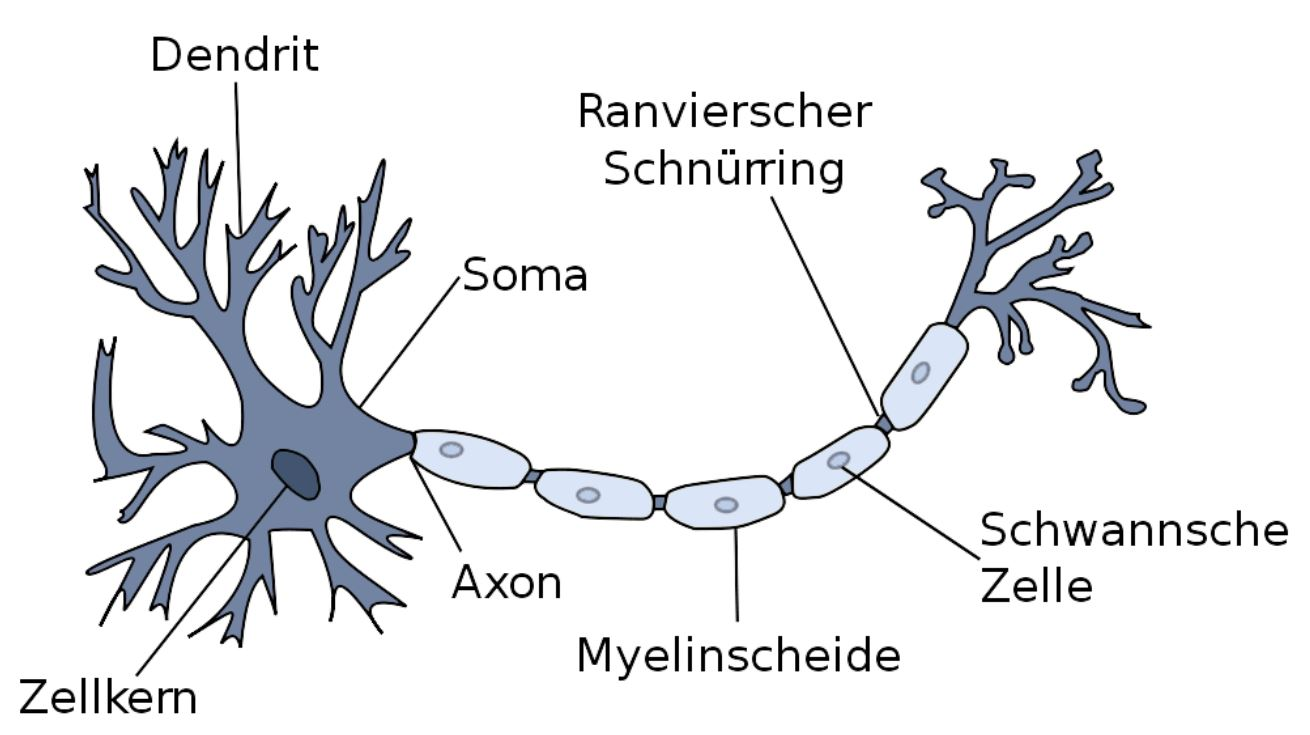
\includegraphics[width=0.75\textwidth]{./img/biologial_neuron.JPG} 
	\caption{Schematische Abbildung einer Nervenzelle \cite{kriesel2008kleiner}.}
	\label{fig:biological_neuron}
\end{figure}
\\ \noindent
Das menschliche Gehirn besitzt ungefähr ${10}^{11}$ einzelne Neuronen, deren schematischer Aufbau in Abbildung \ref{fig:biological_neuron} dargestellt ist. Jedes Neuron besitzt einen Zellkern, der sich im Zellkörper (Soma) befindet. Von dem Zellkörper gehen mehrere Fasern aus, die Dendriten genannt werden \cite{russell2013kunstliche}. An diesen befinden sich Synapsen, welche als Übertragungsstelle fungieren und elektrische oder chemische Signale von Rezeptoren oder anderen Neuronen empfangen \cite{kriesel2008kleiner}. Typischerweise empfängt ein Neuron Signale von 2000 bis 10.000 anderen Nervenzellen \cite{zell2003simulation}.  % TODO 3 mal empfangen
Synapsen, die elektrische Signale erhalten, haben eine starke, direkte, nicht regulierbare Verbindung vom Sender zum Empfänger. Diese sind für hart kodierte Verhaltensmechanismen nützlich, wie zum Beispiel den Fluchtreflex. Die chemische Synapse hingegen ist nicht direkt mit dem Sender verbunden, sondern durch den synaptischen Spalt getrennt. Zur Übertragung eines elektrischen Signals wird dieses auf der präsynaptischen Seite in ein chemisches Signal kodiert, indem Neurotransmitter freigesetzt werden. Diese können über den synaptischen Spalt übertragen und anschließend auf der postsynaptischen Seite wieder in ein elektrisches Signal kodiert werden. Ein großer Vorteil dieser Übertragungsart ist die Regulierbarkeit \cite{kriesel2008kleiner}. Verschiedene Neurotransmitter können unterschiedliche Effekte auf das Neuron haben, beispielsweise anregend (exzitatorisch) oder hemmend (inhibitorisch) wirken \cite{kirschbaum2008biopsychologie}. Zusätzlich kann die Menge der freigesetzten Neurotransmitter die Stärke des Signals beeinflussen \cite{kriesel2008kleiner}. Langfristig gesehen können auch neue Verbindungen bzw. Synapsen entstehen oder alte aufgelöst werden. Es wird angenommen, dass dies die Grundlage des Lernens im menschlichen Gehirn ist \cite{russell2013kunstliche}.
\\\\
Sowohl die anregenden als auch hemmenden Signale werden über die Dendriten an den Axonhügel weitergeleitet, welcher sich zwischen dem Soma und dem Axon befindet. Dort werden die Signale akkumuliert. Beim Überschreiten eines gewissen Schwellwerts wird ein elektrischer Impuls erzeugt, den das Axon weiterleitet \cite{kirschbaum2008biopsychologie}. Das Axon ist typischerweise einen Zentimeter, in Ausnahmen sogar bis zu einem Meter lang und wird von der Myelinscheide umgeben, die unter anderem Schutz vor mechanischer Überbeanspruchung bietet \cite{russell2013kunstliche}. Zusammen mit den Ranvierschen Schnürringen ermöglicht sie zudem eine schnellere Weiterleitung des Aktionspotenzials \cite{kirschbaum2008biopsychologie}. Das Axon endet mit dem sogenannten Endknopf, auch Axonterminal genannt. Dieses ist mit den Synapsen von anderen Neuronen verbunden und setzt beim Eintreffen eines Signals die Neurotransmitter frei, wodurch das Signal übertragen wird \cite{kirschbaum2008biopsychologie}. Typischerweise gibt ein einzelnes Neuron sein Signal an 1000 bis 10.000 andere Neuronen weiter, in Extremfällen sogar an bis zu 150.000 andere Neuronen \cite{zell2003simulation}, die alle parallel arbeiten. So entsteht ein großes und leistungsfähiges neuronales Netz. 

\subsection{Künstliche neuronale Netze}
\ac{KNN} sind ein mathematisches Modell, das im Vergleich zum biologischen Vorbild stark vereinfacht und idealisiert ist. Trotzdem können unterschiedliche mathematische Funktionen abgebildet werden. In diesem Kapitel werden die grundsätzliche Funktionsweise sowie die einzelnen Komponenten der \ac{KNN} vorgestellt.
\begin{figure}[h]
	\centering
	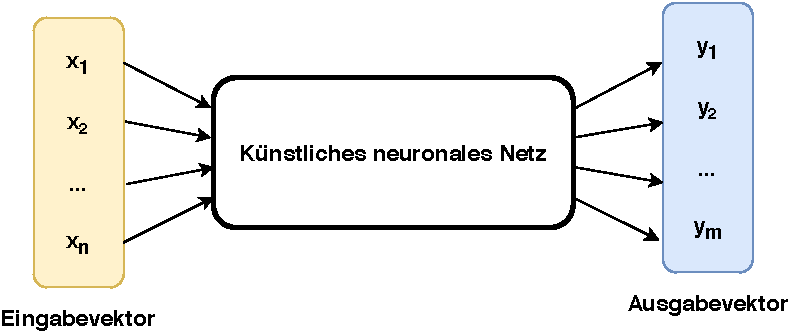
\includegraphics[width=0.6\textwidth]{./img/neural_network_basics/NeuralNetworkBlackbox.pdf} 
	\caption{KNN als Blackbox mit einem Eingabe- und Ausgabevektor}
	\label{fig:neural_network_blackbox}
\end{figure}
\\ \noindent
Betrachtet man ein \ac{KNN} als Blackbox (Abbildung \ref{fig:neural_network_blackbox}), gibt es eine gewisse Anzahl an Eingabewerten, die in einem Eingabevektor kodiert sind und eine Anzahl an Ausgaben, die in einem Ausgabevektor kodiert sind \cite{scherer2013neuronale}. Die Eingaben werden im Fall der \ac{KNN} nicht durch Rezeptoren erfasst, sondern sind durch ein Optimierungsproblem gegeben. Der Ausgabevektor soll das gewünschte Ergebnis enthalten. Je nach Optimierungsproblem kann die Interpretation von diesem variieren. Betrachtet man die Struktur der \ac{KNN}, sind einige Ähnlichkeiten zum biologischen Vorbild erkennbar. Diese werden im Folgenden genauer betrachtet \cite{zell2003simulation}:
\begin{enumerate}
	\item \textbf{Neuronen}\\
	Ähnlich zu den biologischen neuronalen Netzen, besteht auch das \ac{KNN} aus vielen Neuronen \cite{zell2003simulation}. Dies sind einfache Recheneinheiten, die primitive Funktionen bestimmen können \cite{scherer2013neuronale} und deren genaue Funktionsweise in Kapitel \ref{subsec:neuron} erläutert wird. Vorweggenommen sei, dass ein Neuron mehrere Eingabewerte besitzt, welche gewichtet sind und akkumuliert werden. Hierbei entsteht ein skalarer Ausgabewert, der den Aktivierungsgrad des Neurons repräsentiert und von anderen Neuronen als Eingabe verwendet werden kann \cite{kriesel2008kleiner}. 
	 
	\item \textbf{Gerichtete gewichtete Verbindungen}\\
	Wie in der Betrachtung der Neuronen angedeutet, sind diese über gerichtete Verbindungen miteinander vernetzt. Der Aktivierungszustand eines Neurons wird entsprechend der Verbindungen an die Zielneuronen weitergegeben, welche diesen Wert als Eingabe verarbeiten. Wie bei den biologischen neuronalen Netzen auch, können Eingaben unterschiedlich stark anregend oder hemmend wirken. Dies wird bei den \ac{KNN} über Gewichte in den Verbindungen realisiert \cite{zell2003simulation}.
	
	\item \textbf{Struktur und Gewichte}\\
	Der Ausgabevektor eines \ac{KNN} ist abhängig von der Struktur des Netzes und der Gewichte in den einzelnen Verbindungen.
	Für das erfolgreiche Lösen eines Optimierungsproblems muss ein \ac{KNN} die richtige Kombination aus Neuronen, Netzstruktur und gewichteten Verbindungen besitzen. Diese müssen durch Lernverfahren bestimmt werden, auf die in Kapitel \ref{subsec:optimization_strategies} näher eingegangen wird.
\end{enumerate}
Trotz der vorgestellten Ähnlichkeiten sind einige Unterschiede zwischen den biologischen neuronalen Netzen und den \ac{KNN} zu verdeutlichen, für die als Beispiel der Größenunterschied zu nennen ist. Das menschliche Gehirn mit seinen ${10}^{11}$ Neuronen besitzt pro Neuron ungefähr $10^4$ Verbindungen, wogegen die meisten \ac{KNN} nur ${10}^{2}$ bis ${10}^{4}$ Neuronen mit insgesamt ${10}^{5}$ Verbindungen besitzen. Auch werden keine chemischen Effekte, die auf benachbarte Neuronen wirken, sowie zeitliche und räumliche Lokalitätsprinzipien beachtet \cite{zell2003simulation}. Aus diesen Gründen sind die \ac{KNN} keine Nachbildung der biologischen neuronalen Netze, sondern verwenden diese ausschließlich als Inspiration. 

\subsection{Das Neuron}
\label{subsec:neuron}
In diesem Kapitel wird die Funktionsweise der einzelnen Neuronen betrachtet. Hierfür werden drei Phasen, die Propagierungsfunktion, die Aktivierungsfunktion sowie die Ausgabefunktion vorgestellt, in denen der Ausgabewert eines einzelnen Neurons berechnet wird. Betrachtet man ein \ac{KNN}, führen typischerweise mehrere Verbindungen zu einem Neuron $j$, welche von den Neuronen $i_1, i_2, ..., i_n$ ausgehen \cite{kriesel2008kleiner}. Dies ist schematisch in Abbildung \ref{fig:neuron_overview} dargestellt.
\begin{figure}[h]
	\centering
	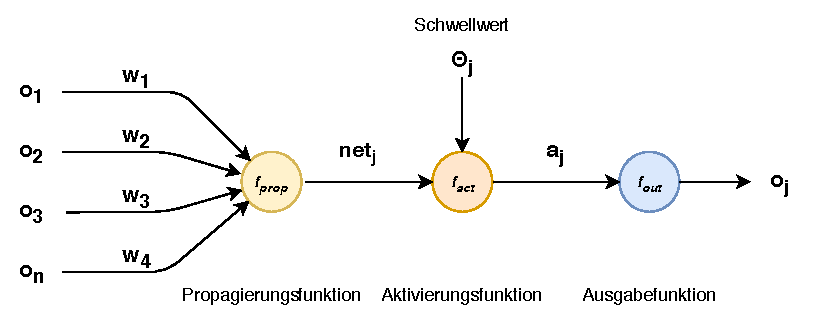
\includegraphics[width=0.9\textwidth]{./img/neural_network_basics/neuron_overview.pdf} 
	\caption{Schematische Darstellung eines einzelnen künstlichen Neurons}
	\label{fig:neuron_overview}
\end{figure}

\subsubsection{Propagierungsfunktion} 
Die Ausgabewerte $o_{i_1}, o_{i_2}, ..., o_{i_n}$ der Neuronen $i_1, i_2, ..., i_n$ werden als Eingabewerte für das Neuron $j$ verwendet. Für jeden Eingabewert existiert ein entsprechendes Gewicht $w_1, w_2, ..., w_n$ \cite{kriesel2008kleiner}. Somit repräsentiert $w_{ij}$ das Gewicht für die Verbindung von Neuron $i$ zu Neuron $j$ \cite{zell2003simulation}. Die Propagierungsfunktion $f_{prop}$ berechnet die Netzeingabe $net_j$, welche in der darauffolgenden Phase weiterverwendet wird \cite{kriesel2008kleiner}. 
$$net_j=f_{prop}(o_1, o_2, ..., o_n, w_1, w_2, ..., w_n)$$
Die meist verwendete Propagierungsfunktion, welche auch in den späteren Beispielen genutzt wird, ist die gewichtete Summe. Hierbei werden entsprechend der Formel die Werte $o_i$ mit dem entsprechenden Gewicht $w_i$ multipliziert und aufsummiert \cite{kriesel2008kleiner}:
$$net_j=\sum_{i}(o_{i} \cdot w_{i, j})$$

\subsubsection{Aktivierungsfunktion}
\label{subsubsec:activatoin_function}
Der Aktivierungszustand $a_j(t)$ gibt den Grad der Aktivierung von Neuron $j$ zum Zeitpunkt $t$ an. Ein neuer Aktivierungszustand zum Zeitpunkt $t+1$ wird mit der Aktivierungsfunktion $f_{act}$ berechnet. Diese berücksichtigt nicht nur die Netzeingabe $net_j(t)$, sondern auch den vorherigen Aktivierungszustand $a_j(t)$ und den Schwellwert $\Theta$ der Aktivierungsfunktion \cite{zell2003simulation}. Ein Schwellwert $\Theta_j$, auch \emph{Bias} genannt, ist dem Neuron $j$ zugeordnet und gibt die Stelle an, an welcher die Aktivierungsfunktion die größte Steigung hat \cite{kriesel2008kleiner}. Somit kann die Berechnung der Aktivierung $a_j(t+1)$ durch folgende Formel ausgedrückt werden \cite{zell2003simulation}:
$$a_j(t+1)=f_{act}(a_j(t), net_j, \Theta_j)$$
Bei der Berechnung kommt dem Schwellwert $\Theta$ eine besondere Bedeutung zu. Oftmals verwenden einige oder alle Neuronen eines \ac{KNN} dieselbe Aktivierungsfunktion, die Schwellwerte hingegen unterscheiden sich je nach Neuron. Des Weiteren sei angemerkt, dass die vorherige Aktivierung $a_j(t)$ je nach Netzstruktur oft keine Berücksichtigung bei der Berechnung findet \cite{kriesel2008kleiner}. Zudem wird in der Praxis bei Verwendung der gewichteten Summe als Propagierungsfunktion der Schwellwert eines Neurons oft schon in der ersten Phase miteinbezogen. Hierdurch ändert sich die Berechnung der Netzeingabe zu $net_j=\sum_{i}(o_{i} \cdot w_{i, j}) - \Theta_j$. Bei der Berechnung der Aktivierungsfunktion gilt dann $\Theta_j = 0$.
\\\\
Je nach Anwendungsgebiet können verschiedene Aktivierungsfunktionen mit unterschiedlichen Eigenschaften eingesetzt werden. Vier Beispiele sind im Folgenden vorgestellt, für die angenommen wird, dass $\Theta_j=0$ ist. Das einfachste Beispiel für eine Aktivierungsfunktion ist die sogenannte binäre Schwellwertfunktion, welche nur die Werte $0$ und $1$ zurückgeben kann \cite{kriesel2008kleiner}. Die Formel hierfür ist: 
$$
f_{act}(net_j)=\left\{\begin{array}{ll}
1 & \text { wenn } net_j \geq 0 \\
0 & \text { wenn } net_j < 0
\end{array}\right.
$$
Allerdings ist für diese Funktion der Wert der Ableitung immer $0$, ausgenommen an dem Schwellwert, an welchem sie nicht differenzierbar ist. Diese Eigenschaften machen sie ungeeignet für bestimmte Lernverfahren, wie zum Beispiel den Backpropagation Algorithmus, auf den in Kapitel \ref{subsec:backprop_algo} kurz eingegangen wird \cite{kriesel2008kleiner}. \\\\
Dieses Problem kann durch die Verwendung einer Sigmoidfunktion gelöst werden. Zwei bekannte Beispiele für Sigmoidfunktionen sind die logistische Funktion und der \ac{tanh} \cite{lecun2012efficient}. Die logistische Funktion kann Werte von 0 bis 1 annehmen und wird berechnet durch \cite{kriesel2008kleiner}: 
$$f_{act}(net_j)=\frac{1}{1+e^{-net_j}}$$
Allerdings können neuronale Netze je nach Verfahren schneller optimiert werden, wenn das durchschnittliche Gewicht aller Verbindungen nahe 0 ist. In diesem Fall kann die \ac{tanh} Funktion besser geeignet sein, da sie Werte zwischen -1 und 1 annehmen kann \cite{lecun2012efficient}. Das abschließend vorgestellte Beispiel ist die sogenannte \emph{Rectifier}-Funktion. Diese wird oft in Zusammenhang mit dem Backpropagation Algorithmus erfolgreich eingesetzt \cite{glorot2011deep}. Berechnet wird sie durch:
$$f_{act}(net_j)= max(0, net_j)$$

\subsubsection{Ausgabefunktion}
Die Ausgabefunktion $f_{out}$ berechnet die Ausgabe $o_j$ von Neuron $j$. Als Eingabewert wird die Aktivierung $a_j$ verwendet \cite{zell2003simulation}. Definiert ist die Funktion durch:
$$o_j = f_{out}(a_j)$$
Ähnlich der Aktivierungsfunktion ist die Ausgabefunktion in der Praxis meist global für alle Neuronen definiert. Als eine solche Ausgabefunktion wird häufig die Identitätsfunktion verwendet, für welche $o_j = a_j$ gilt \cite{kriesel2008kleiner}. Diese kommt auch in den später vorgestellten Beispielen zur Anwendung. Ist die Ausgabe $o_j$ berechnet, kann sie als Eingabewert für andere verbundene Neuronen dienen.

\subsection{Netzstrukturen}
\label{subsec:network_structures}
Aus dem vorherigen Kapitel wird deutlich, dass die Gewichte einen großen Einfluss auf den Ausgabewert eines einzelnen Neurons haben. Der Ausgabevektor eines \ac{KNN} wird zusätzlich von der Anzahl an Neuronen sowie deren Verbindungsstruktur beeinflusst. Dieses Kapitel führt verschiedene Varianten ein, die je nach Optimierungsproblem eingesetzt werden können. 
\\\\
Typischerweise besitzt jedes \ac{KNN} Eingabe- und Ausgabeneuronen. Optional kann ein \ac{KNN} beliebig viele verdeckte Neuronen enthalten. Diese werden auch als \emph{Input}-, \emph{Output}- und \emph{Hidden}-Neuronen bezeichnet \cite{zell2003simulation}. Die Anzahl der Eingabe- und Ausgabeneuronen ist abhängig von der Größe des Eingabe- bzw. Ausgabevektors. Für jedes Element in den Vektoren gibt es ein entsprechendes Neuron.
Bei vielen Netzstrukturen werden die Neuronen des \ac{KNN} verschiedenen Schichten zugeordnet. In der ersten Schicht befinden sich die Eingabeneuronen, in der letzten die Ausgabeneuronen. Dazwischen befinden sich $n$ Schichten mit verdecken Neuronen \cite{zell2003simulation}. 
\\\\
Bei der Berechnung eines \ac{KNN} werden zuerst die Werte des Eingabevektors in die entsprechenden \emph{Input}-Neuronen eingesetzt. Anschließend werden alle Neuronen in einer bestimmten Reihenfolge aktiviert bzw. berechnet. Zuletzt bilden die Werte der \emph{Output}-Neuronen den Ausgabevektor. Die \emph{Hidden}-Neuronen, deren Bezeichnung darin begründet ist, dass ihr Ausgabewert nur ein Zwischenergebnis darstellt und vor dem Anwender verborgen bleibt, befinden sich zwischen den \emph{Input}- und \emph{Output}-Neuronen. Trotzdem sind sie ein elementarer Bestandteil der \ac{KNN} und bestimmen maßgeblich deren Leistungsfähigkeit. Beispielsweise kann ein aus \emph{Input}- und \emph{Output}-Neuronen bestehendes \ac{KNN} nur eine lineare Funktion repräsentieren. Ein \ac{KNN} mit einer ausreichend großen verdeckten Schicht kann jede beliebige kontinuierliche Funktion darstellen. Mit zwei Schichten kann ein \ac{KNN} sogar jede unstetige mathematische Funktion mit beliebiger Genauigkeit abbilden \cite{russell2013kunstliche}. Je nach Art des Verbindungsmusters zwischen den Neuronen werden \ac{KNN} einer von zwei Gruppen zugeordnet. Die erste Gruppe enthält Netze ohne Rückkopplung, welche auch \emph{feedforward}-Netze genannt werden. Die zweite Gruppe sind die sogenannten \emph{recurrent}-Netze, zu welchen \ac{KNN} mit Rückkopplungen gehören \cite{zell2003simulation}.

\subsubsection{Netze ohne Rückkopplung}
Die Definition der \emph{feedforward}-Netze sieht vor, dass es keine Verbindung geben darf, die von einem Neuron $j$ ausgeht und wieder zu sich selbst führt. Dabei ist es irrelevant, ob eine direkte oder indirekte Verbindung über Zwischenneuronen besteht. Es entsteht ein azyklischer Graph \cite{zell2003simulation} und das \ac{KNN} kann infolgedessen keinen internen Zustand besitzen. Für die gleiche Eingabe wird immer dasselbe Ergebnis berechnet. Innerhalb dieser Kategorie gibt es zwei Untergruppen, die ebenenweise verbundenen \ac{KNN} und die \ac{KNN}, welche über sogenannte \emph{shortcut} Verbindungen verfügen.
\begin{figure}[h]
	\centering
	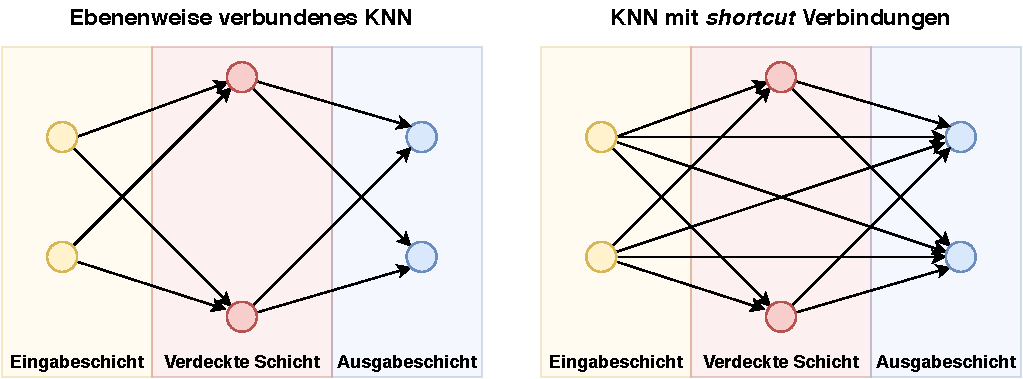
\includegraphics[width=1.0\textwidth]{./img/neural_network_basics/feed_forward_networks.pdf} 
	\caption{Links ein ebenenweise verbundenes \emph{feedforward} KNN, rechts ein KNN mit \emph{shortcut} Verbindungen}
	\label{fig:feed_forward_network_structures}
\end{figure}
Bei den rein ebenenweise verbundenen \ac{KNN} stammen die Eingabewerte eines Neurons immer aus der vorherigen Schicht. Der berechnete Ausgabewert eines Neurons wird nur an die Neuronen der nächsten Schicht weitergeleitet \cite{zell2003simulation}. Ein Beispiel hierfür ist in Abbildung \ref{fig:feed_forward_network_structures} links dargestellt. Im Gegensatz dazu stehen die \ac{KNN} mit \emph{shortcut} Verbindungen. Wie in Abbildung \ref{fig:feed_forward_network_structures} rechts dargestellt, können \emph{shortcut} Verbindungen eine oder mehrere Schichten überspringen. Für gewisse Optimierungsprobleme, unter anderem für das in Kapitel \ref{sec:analysis_valdation_functionality} dargestellte XOR-Problem, können so kleinere \ac{KNN} erzeugt werden \cite{zell2003simulation}. 

\subsubsection{Netze mit Rückkopplung}
Durch rückgekoppelte Verbindungen entstehen Zyklen in der Berechnung, wodurch sich das \ac{KNN} selbst beeinflussen kann. Damit ist unter anderem das Zwischenspeichern von Ergebnissen möglich \cite{russell2013kunstliche}. Somit kann die Berechnung des Ausgabevektors sowohl durch die Eingabewerte als auch durch die vorherigen Ergebnisse beeinflusst werden \cite{lin1998embedded}. Wie die \emph{feedforward}-Netze können auch die Netze mit Rückkopplungen je nach Verbindungsart verschiedenen Untergruppen zugeordnet werden \cite{zell2003simulation}. Diese sind in Abbildung \ref{fig:recurrent_network_structures} dargestellt und im Folgenden beschrieben.
\begin{figure}[h]
	\centering
	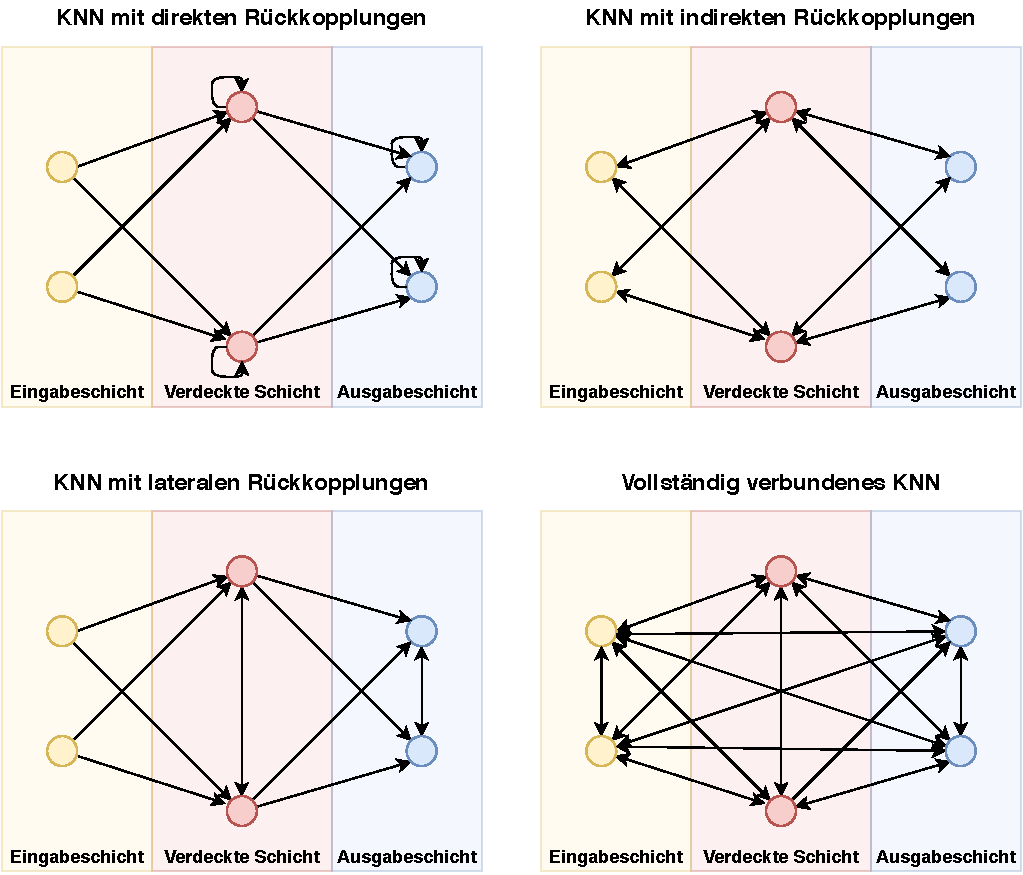
\includegraphics[width=1.0\textwidth]{./img/neural_network_basics/recurrent_networks.pdf} 
	\caption{Schematische Darstellung des Verbindungsmusters von verschiedenen KNN mit Rückkopplungen}
	\label{fig:recurrent_network_structures}
\end{figure}
\begin{enumerate}
	\item Bei \ac{KNN} mit direkten Rückkopplungen können Neuronen Verbindungen zu sich selbst haben und hierdurch ihre eigene Aktivierung verstärken oder abschwächen \cite{zell2003simulation}.
	\item Netze mit einer indirekten Rückkopplung erlauben im Gegensatz zu den \emph{feedforward}-Netzen auch Verbindungen in die vorherige Schicht \cite{zell2003simulation}. Wie bei der direkten Rückkopplung kann sich ein Neuron $j$ selbst beeinflussen, wenn es seinen Ausgabewert an ein Neuron $i$ der nächsten Schicht weiterleitet, welches eine Rückkopplung zu $j$ hat \cite{kriesel2008kleiner}.
	\item \ac{KNN} mit lateralen Rückkopplungen erlauben Verbindungen von Neuronen innerhalb einer Schicht, welche hemmend oder aktivierend wirken können. Oft entsteht dabei ein \emph{Winner-Takes-All}-Schema, da das beste Neuron alle anderen hemmt und sich selbst aktiviert \cite{kriesel2008kleiner}.
	\item Bei den vollständig verbundenen Netzen darf ein Neuron zu jedem anderen eine Verbindung besitzen. Ein Sonderfall sind hier die sogenannten Hopfield-Netze. Bei diesen müssen die Neuronen zu jedem anderen eine Verbindung besitzen mit Ausnahme zu sich selbst \cite{kriesel2008kleiner}.  
\end{enumerate}

\subsection{Optimierungsmöglichkeiten}
\label{subsec:optimization_strategies}
In den vorherigen Kapiteln ist aufgezeigt, dass das erfolgreiche Lösen eines Optimierungsproblems mit einem \ac{KNN} von vielen Faktoren abhängt. In der Praxis ist eine manuelle Bestimmung dieser bei komplexen Aufgaben nicht möglich. Aus diesem Grund muss ein Optimierungsverfahren, welches auch als Lernverfahren bezeichnet wird, angewendet werden. Ziel von diesem ist, einen Teil oder alle Parameter des \ac{KNN} durch einen Algorithmus automatisch zu bestimmen. Typischerweise ist das Lernverfahren unabhängig vom eigentlichen Optimierungsproblem und kann daher in verschiedenen Bereichen ohne großen zusätzlichen Aufwand eingesetzt werden. 
\\\\
Ein Lernverfahren kann theoretisch auf vier verschiedene Arten die Eigenschaften eines \ac{KNN} optimieren \cite{zell2003simulation}. Diese sind im Folgenden kurz zusammenfasst.
\begin{enumerate}
	\item \textbf{Modifizieren der Verbindungsgewichte}:\\
	Die Gewichte der einzelnen Verbindungen werden in der Praxis von allen Lernverfahren optimiert \cite{zell2003simulation}. Gründe hierfür sind, dass ein \ac{KNN} mehrere Millionen Verbindungen besitzen kann, welche unmöglich manuell optimiert werden können, und dass die Gewichte entscheidend für die erfolgreiche Optimierung sind.

	\item\textbf{Modifizieren der Schwellwerte}:\\
	Die Schwellwerte der Neuronen werden wie die Gewichte von den meisten Lernverfahren optimiert. In der Praxis ist der hierbei verwendete Vorgang oft identisch mit der Gewichtsoptimierung. Dies ist möglich, wenn, wie in einigen Implementierungen umgesetzt, die Schwellwerte durch Gewichte repräsentiert werden. Hierzu wird einem \ac{KNN} ein sogenanntes \emph{Bias}-Neuron hinzugefügt, welches immer den Wert 1 hat. Von diesem gehen Verbindungen zu allen Neuronen aus. Der Schwellwert $\Theta_j$ von einem Neuron $j$ wird durch das Gewicht $w_{\Theta j}$ repräsentiert. Dieses ist der eingehenden Verbindung vom \emph{Bias}-Neuron zugeordnet, sodass gilt $1\cdot w_{\Theta j} = \Theta_j$. Dadurch muss bei der Berechnung eines Neurons der Schwellwert nicht mehr explizit miteinbezogen werden, sondern wird im Rahmen der Propagierungsfunktion indirekt mit den anderen gewichteten Eingaben verarbeitet. Bezüglich der Optimierung wird die Verbindung zum \emph{Bias}-Neuron wie andere gewichtete Verbindungen behandelt \cite{zell2003simulation}.

	\item \textbf{Hinzufügen und Entfernen von Verbindungen oder Neuronen}:\\
	Das Hinzufügen beziehungsweise Entfernen von Verbindungen und Neuronen ist im Vergleich zu den bereits vorgestellten Möglichkeiten aufwändig und in der Umsetzung schwieriger. Daher ist es in vielen bekannten Algorithmen nicht implementiert. Bei diesen muss die Struktur mithilfe von Expertenwissen oder Erfahrung festgelegt werden \cite{stanley2017oreilly}, andernfalls ist eine geeignete Struktur experimentell zu ermitteln. Da dieses Vorgehen häufig nicht effizient ist, gibt es dennoch einige Algorithmen, die das Hinzufügen und Entfernen von Strukturen bei der Optimierung nutzen. Diese gehören oft zu der Klasse der neuroevolutionären Algorithmen, auf welche in Kapitel \ref{subsec:neuroevolution} eingegangen wird \cite{kriesel2008kleiner}.
	
	\item \textbf{Ändern der Propagierungs-, Aktivierungs- und Ausgabefunktion}:\\
	Die Optimierung der verwendeten Propagierungs-, Aktivierungs- und Ausgabefunktion ist theoretisch möglich, die Umsetzung ist in der Praxis allerdings nicht sehr verbreitet \cite{zell2003simulation}. Auch in dieser Arbeit werden diese Funktionen nicht durch einen Algorithmus angepasst und daher nicht weiter betrachtet. 
\end{enumerate}

\subsection{Arten von Optimierungsverfahren}
\label{subsec:learning_in_neural_networks}
In Kapitel \ref{subsec:optimization_strategies} sind Optimierungsmöglichkeiten aufgelistet, welche von einem Lernverfahren in der sogenannten Trainingsphase des \ac{KNN} angepasst werden können. Ziel ist, dass am Ende dieser Phase der Ausgabevektor des \ac{KNN} dem gewünschten Ergebnis entspricht. Voraussetzung hierfür ist, dass das gewünschte Ergebnis erkennbar ist \cite{zell2003simulation}. Bei den Lernverfahren wird grundsätzlich zwischen dem überwachten, unüberwachten und bestärkenden Lernen differenziert, welche unterschiedliche Arten des Lernens für verschiedene Aufgabenstellungen repräsentieren. Im Folgenden wird ein Überblick über diese gegeben. Für eine genaue Beschreibung und die dazugehörigen Algorithmen wird auf entsprechende Fachliteratur verwiesen.

\subsubsection{Überwachtes Lernen}
\label{subsubsec:supervised_learning}
Das überwachte Lernen, auch \emph{supervised learning} genannt, wird häufig mit dem Backpropagation Algorithmus und seinen Derivaten umgesetzt und beruht auf bekannten Beispieldaten. Diese müssen in großer Anzahl schon vor dem Lernvorgang vorhanden sein und den Eingabevektor sowie den gewünschten Ausgabevektor des \ac{KNN} enthalten \cite{zell2003simulation}. In der sogenannten Trainingsphase, analysiert das Lernverfahren die vorhanden Beispieldaten mit dem Ziel Muster zu extrahieren. Am Ende der Trainingsphase soll das \ac{KNN} nicht nur die korrekte Lösung für die bekannten Beispiele angeben können, sondern auch für ähnliche, unbekannte Eingabedaten. Damit ist die Eigenschaft der Generalisierung erfüllt. \cite{zell2003simulation}. Um den Erfolg des Verfahrens zu überprüfen, werden die Beispieldaten in Trainings- und Testdaten unterteilt. Die Trainingsphase wird nur mit den Trainingsdaten durchgeführt, sodass die Testdaten dem \ac{KNN} unbekannt sind. Ist diese Phase abgeschlossen, weil beispielsweise das \ac{KNN} eine gute Genauigkeit erreicht hat, werden die Testdaten zur Validierung eingesetzt. Hierbei wird überprüft, ob das \ac{KNN} auch für unbekannte Eingabevektoren die richtigen Ergebnisse berechnet \cite{kriesel2008kleiner}. Diese Art des Lernens ist im Vergleich zu den anderen Varianten sehr schnell \cite{zell2003simulation}, aber das Anwenden ist nicht in jeder Situation möglich. Liegen keine Beispiele vor, kann das \ac{KNN} nicht trainiert werden. Sind die Beispieldaten fehlerhaft oder verrauscht, kann das Training langsam, nicht zufriedenstellend oder unmöglich sein.

\subsubsection{Unüberwachtes Lernen}
\label{subsubsec:unsupervised_learning}
Beim unüberwachten Lernen, auch \emph{unsupervised learning} genannt, stehen ebenfalls Beispieldaten zur Verfügung, allerdings enthalten diese nur den Eingabevektor und keine dazugehörigen Ausgabevektoren. Ziel solcher Lernverfahren ist, Muster in den Eingabedaten automatisch zu erkennen und diese verschiedenen Gruppen zuzuordnen, sodass sich ähnelnde Eingabewerte derselben Gruppe zugewiesen werden \cite{zell2003simulation}. Solche Verfahren können einige Vorteile gegenüber dem überwachten Lernen bieten \cite{mahmad2005IEEE}. Zum Beispiel müssen vor dem Training keine Beispieldaten mit Ausgabevektoren vorliegen, welche teilweise sehr teuer und aufwendig zu erstellen sind. Des Weiteren kann je nach Algorithmus die Anzahl an vorhandenen Gruppen automatisch zugewiesen werden. So können auch unterschwellige Muster, die nicht von einem Menschen erkannt werden würden, die Zuweisung beeinflussen \cite{mahmad2005IEEE}.
 
\subsubsection{Bestärkendes Lernen}
\label{subsubsec:reinforcment_learning}
Die letzte Klasse ist das bestärkende Lernen, auch \emph{reinforcment learning} genannt. Typischerweise wird diese Art des Lernens in dynamischen Umgebungen eingesetzt, in welcher ein sogenannter Agent mit einer Umgebung interagiert. Ein häufig genannter Begriff in diesem Kontext ist der \ac{MDP}, welcher in Abbildung \ref{fig:mdp_problem} dargestellt ist und anhand dessen im Folgenden das bestärkende Lernen beschrieben ist \cite{sutton2018reinforcement}. 
\begin{figure}[h]
	\centering
	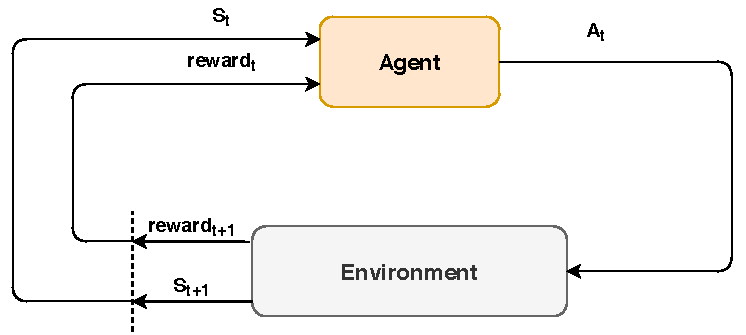
\includegraphics[width=0.7\textwidth]{./img/neural_network_basics/mdp.pdf} 
	\caption{Interaktion des Agenten mit der Umgebung im MDP}
	\label{fig:mdp_problem}
\end{figure}
\\ \noindent
Zwei wichtige Grundkomponenten des \acp{MDP} sind der Agent und die Umgebung. Der aktuelle Zustand der Umgebung zu einem Zeitpunkt $t$ wird durch die Variable $S_t$ repräsentiert. Ist die Umgebung zum Beispiel ein Computerspiel, kann $S_t$ unter anderem die aktuelle Position sowie Zielkoordinaten enthalten. Der Zustand $S_t$ steht dem Agenten zur Verfügung, der daraufhin eine Aktion $A_t$ ausführt. Als Basis für die Entscheidung kann ein \ac{KNN} dienen, welches als Eingabevektor den aktuellen Zustand verwendet und einen Ausgabevektor mit der gewählten Aktion erzeugt. Die verfügbaren Aktionen sind je nach System unterschiedlich. So können zum Beispiel bei der Steuerung von Robotern sowohl direkte Steuersignale für die Motoren ausgegeben werden als auch \emph{high-level} Entscheidungen wie die Bewegungsrichtung. Nach Ausführung der Aktion wird der Zustand der Umgebung entsprechend angepasst und ein neuer Zustand $S_{t+1}$ entsteht \cite{sutton2018reinforcement}, für den der Agent eine neue Aktion auswählen kann. Zusätzlich wird ein Belohnung, auch als $reward$ bezeichnet, vergeben. Dies ist ein numerischer Wert, der angibt, wie richtig oder falsch die gewählte Aktion war \cite{zell2003simulation}. Eine richtige Aktion zeichnet sich dadurch aus, dass sie den Agenten näher an sein gewünschtes Ziel bringt. Im zuvor genannten Beispiel des Computerspiels ist der \emph{reward} größer, wenn der Agent die Distanz zum Ziel verringert und kleiner bzw. negativ, wenn der Agent sich wieder entfernt. Ziel eines Optimierungsalgorithmus ist, die Summe der erhaltenen Belohnungen zu maximieren. Hierdurch ergeben sich komplexe Anforderungen an das Lernverfahren. Bei der Entscheidung, welche Aktion $A_t$ bei einem Zustand $S_t$ den meisten Erfolg verspricht, muss sowohl der direkte als auch zukünftige \emph{reward} berücksichtigt werden \cite{sutton2018reinforcement}. Dies ist notwendig, da ein Agent viele Aktionen in derselben sich ändernden Umgebung ausführt und eine Entscheidung Auswirkungen auf die Zukunft hat. Somit kann es bei vielen Optimierungsproblemen  lohnenswert sein, zur Schaffung einer besseren Ausgangslage zuerst eine schlechte Belohnung in Kauf zu nehmen, sodass im weiteren Verlauf größere Belohnungen erreicht werden können. Eine weitere Herausforderung für solche Algorithmen ist, dass ein Gleichgewicht zwischen dem Nutzen von Erfahrung und Ausprobieren gefunden werden muss. Möglichst hohe Belohnungen kann ein Agent nur erhalten, wenn er bekannte Entscheidungen trifft, die in der Vergangenheit erfolgreich waren. Allerdings müssen auch neue unbekannte Aktionen ausgewählt werden, da diese unter Umständen besser sein können. Für ein gutes Lernverfahren ist es notwendig, eine Kombination aus beidem zu ermöglichen \cite{sutton2018reinforcement}. Bei vielen Optimierungsproblemen wird das bestärkende Lernen erfolgreich eingesetzt. Ein Nachteil jedoch ist die lange Laufzeit im Vergleich zu anderen Verfahren, wie zum Beispiel dem überwachtem Lernen. Grund hierfür ist, dass eine niedrige Belohnung keine Aussage darüber trifft wie das \ac{KNN} optimiert werden soll um bessere Ergebnisse zu erzielen. Anpassungen können sich sowohl positiv als auch negativ auf den Agenten auswirken \cite{zell2003simulation}. 


\subsection{Backpropagation Algorithmus}
\label{subsec:backprop_algo}
???

%Während der Optimierung erhält das \ac{KNN} Beispieldaten, für welche der Ausgabevektor berechnet wird. Für das berechnete %Ergebnis wird ein Feedback gegeben, welches auch als \emph{reward} bezeichnet wird. Dieses gibt an, ob der Ausgabewert korrekt %ist beziehungsweise wie richtig oder falsch. Das Lernverfahren muss mit diesen Angaben das \ac{KNN} optimieren, kann aber nicht %wissen wie die Gewichte und je nach Algorithmus die Struktur verändert werden müssen. Dies ist auch der Grund, warum diese Art %des Lernens im Vergleich zum überwachtem Lernen sehr langsam ist, da die Gewichte nicht gezielt angepasst werden können %\cite{zell2003simulation}.\\
%Das Einsatz

% Agent Scenario, Agent must explore/take known actions = trade off, Reward funktion ist anpassbar, muss nicht so sein. 
% file:///D:/Dropbox/Studium%20Master/Semester%203/Masterthesis%20Quellen/Neuroevolution%20strateies%20for%20episodic%20reinforcment%20learning.pdf
% "C:\Users\Simon Hauck\Downloads\Neuroevolution strateies for episodic reinforcment learning.pdf"
\section{Evolutionäre Algorithmen}
\subsection{Genome und Phenom}
\subsection{Phasen des Algos}
\subsection{Kodierung}
\subsection{Competing Convention Problem}
% !TeX spellcheck = de_DE
\section{NeuroEvolution of Augmenting Topologies}
\label{sec:neat}
Der in dieser Arbeit verwendete Algorithmus heißt \ac{NEAT}, welcher im Jahr 2002 von \citeauthor{stanley2002evolving} vorgestellt wurde. Bei der Veröffentlichung hat \ac{NEAT} für die meisten Optimierungsprobleme im Vergleich zu anderen Verfahren schneller Lösungen gefunden, obwohl es neben den Gewichten des \ac{KNN} auch die Struktur optimiert \cite{stanley2002evolving}. Somit gehört der Algorithmus zur Gruppe der \ac{TWEANN} Algorithmen. Heute gilt \ac{NEAT} immer noch als einer der bekanntesten Vertretern der neuroevolutionären Algorithmen und dient als Basis für viele Erweiterungen wie zum Beispiel HyperNEAT, cgNEAT, ... \\
% TODO Add NEAT Sources
Für die guten Ergebnisse sind drei Eigenschaften besonders relevant \cite{stanley2002evolving}:
\begin{enumerate}
	\item Erfolgreiche Reproduktion trotz verschiedener Strukturen
	\item Schützen von neuen Innovationen durch verschiedene Spezies
	\item Wachsen einer minimalen Struktur
\end{enumerate}
In diesem Kapitel wird die grundsätzliche Funktionsweise von \ac{NEAT} erläutert, wie sie in der originalen Publikation vorgestellt ist. Wenn nicht anderweitig gekennzeichnet, beziehen sich alle Informationen aus diesem Kapitel auf Quelle \cite{stanley2002evolving}. Für eine bessere Lesbarkeit wird in diesem Kapitel auf weitere Zitierungen verzichtet.
\subsection{Kodierung}
\label{subsec:neat_encoding} % TODO ABBILDUNG
\begin{figure}[!h]
	\centering
	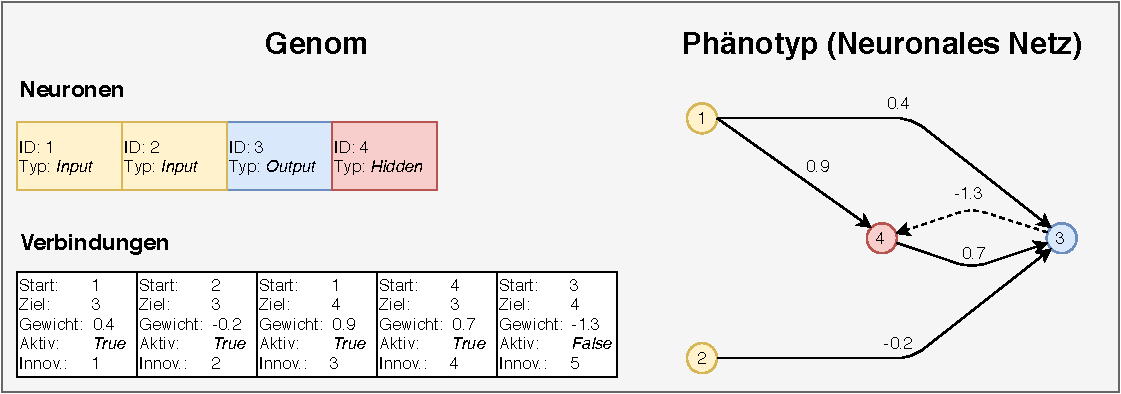
\includegraphics[width=1\textwidth]{./img/neat_genome_encoding.pdf} 
	\caption{Schematische Darstellung von einem Genom mit dazugehörigem Phänotyp}
	\label{fig:neat_encoding}
\end{figure}
\ac{NEAT} verwendet ein direktes Kodierungsverfahren. Ein Genom enthält, wie in Abbildung (TODO ABBILDUNG) beispielhaft dargestellt, je eine Liste für Neuronen und Verbindungen. Ein Neuron wird durch eine ID identifiziert und enthält den Typ (\emph{Input}, \emph{Output}, \emph{Hidden}). Eine Verbindung enthält das Start- und Zielneuron, das dazugehörige Gewicht, ein Aktivierungsbit sowie eine Innovationsnummer. Das Aktivierungsbit gibt an, ob die Verbindung im Phänotyp, in diesem Fall dem neuronalen Netz enthalten, ist. Auf die Funktionsweise und Bedeutung der Innnovationsnummer wird später genauer eingegangen.
\subsection{Mutation}
\label{subsec:neat_mutation}
Ein Genom kann auf verschiedene Arten mutieren, welche entweder die Struktur des \ac{KNN} oder die Gewichte der Verbindungen beeinflussen. Die Mutation der Gewichte ist ähnlich zu anderen neuroevolutionären Algorithmen. Für jedes Gewicht besteht eine Wahrscheinlichkeit zur Mutation. In diesem Fall wird das Gewicht entweder leicht abgeändert oder ein neuer zufälliger Wert gewählt.\\ % TODO ABBILDUNG
\begin{figure}[!h]
	\centering
	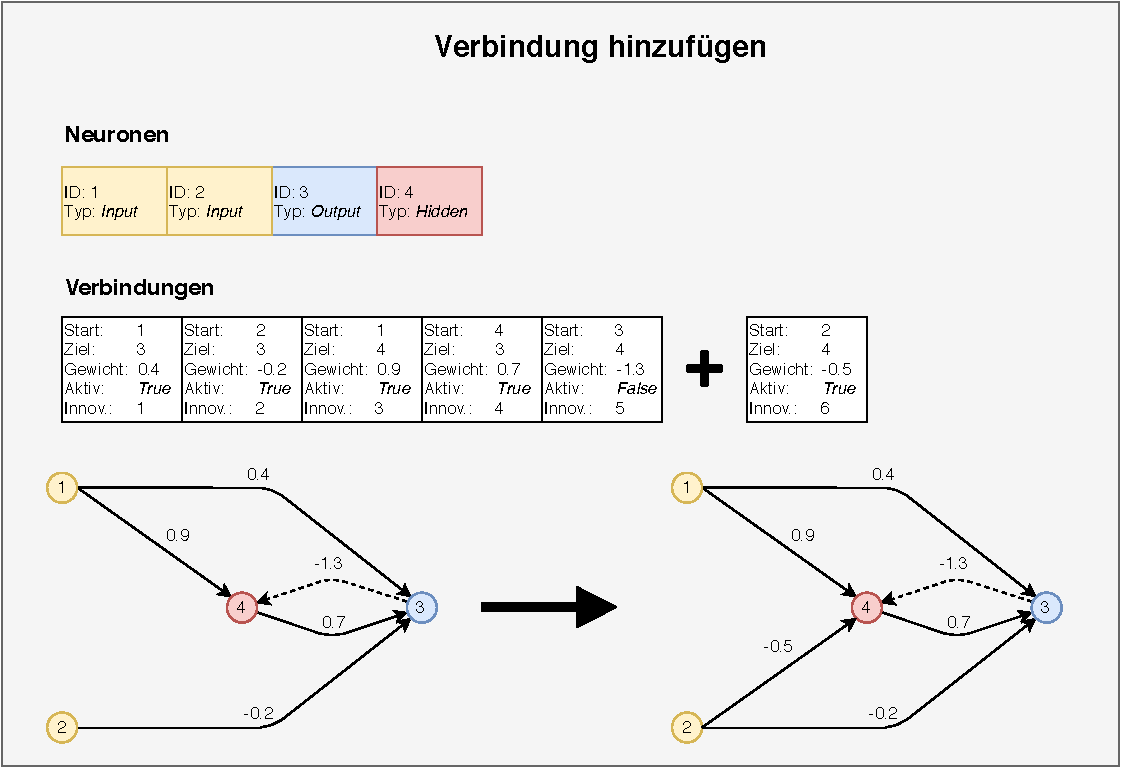
\includegraphics[width=1\textwidth]{./img/neat-AddConnectionMutation.pdf} 
	\caption{Schematische Darstellung von einem Genom mit dazugehörigem Phänotyp}
	\label{fig:neat_add_connectin_mutation}
\end{figure}
Strukturelle Mutationen können in zwei verschiedenen Arten auftreten. Bei der ersten wird eine einzelne neue Verbindung dem Genom hinzugefügt. Bei der Auswahl des Start- und Zielneurons ist zu beachten, dass diese nicht bereits über eine solche Verbindung verfügen. Das Gewicht für die neue Verbindung wird zufällig gewählt und das Aktivierungsbit auf \emph{True} gesetzt. Ein Beispiel für diese Mutation ist in Abbildung (TODO ABBILDUNG) dargestellt. Bei der zweiten Art der strukturellen Mutation wird ein neues Neuron in das \ac{KNN} eingefügt. Hierzu wird zu Beginn eine aktive Verbindung $con_{ij} $ zufällig ausgewählt, welche von Neuron $i$ zu Neuron $j$ führt. Anschließend wird ein neues Neuron $x$ zwischen den Neuronen $i$ und $j$ platziert und zwei weitere Verbindungen werden hinzugefügt. Die erste Verbindung $con_{ix}$ führt vom alten Startneuron $i$ zum neu hinzugefügtem und erhält das Gewicht $1$. Die zweite Verbindung $con_{xj}$ beginnt bei dem neuen Neuron und endet im dem alten Zielneuron $j$ und erhält dasselbe Gewicht wie die Verbindung $con_{ij}$. Zuletzt wird die ausgewählte Verbindung $con_{ij}$ deaktiviert, indem das Aktivierungsbit auf $False$ gesetzt wird. Diese Art der Mutation reduziert den initialen Effekt des neuen Neurons. So kann es direkt vom \ac{KNN} verwendet werden, ohne dass die Verbindungsgewichte stark optimiert werden müssen.
\begin{figure}[!h]
	\centering
	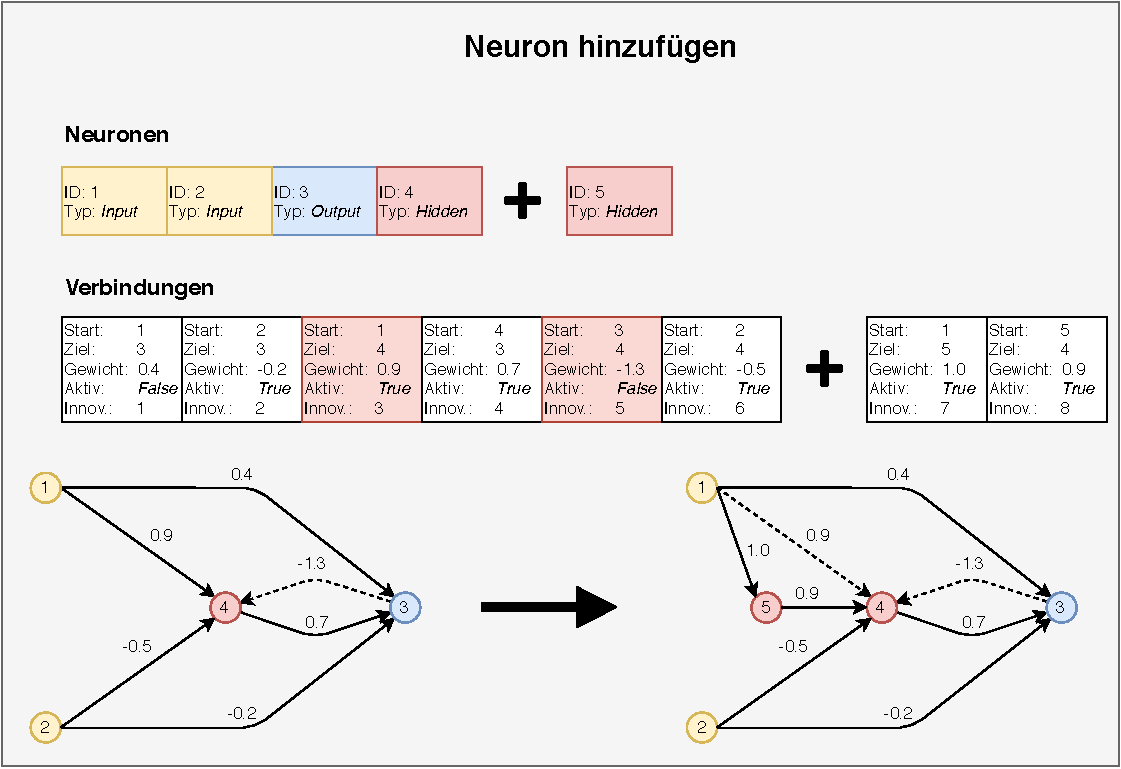
\includegraphics[width=1\textwidth]{./img/neat-AddNodeMutation.pdf} 
	\caption{Schematische Darstellung von einem Genom mit dazugehörigem Phänotyp}
	\label{fig:neat_add_node_mutation}
\end{figure}
\subsection{Reproduktion}
\label{subsec:neat_reproduction}
Das Ergebnis der in Kapitel \ref{subsec:neat_mutation} vorgestellten Mutationen ist eine Population mit verschieden Genomen, welche unterschiedliche Gewichte und Strukturen haben können. Dies ist die schwierigste Form des in Kapitel \ref{subsec:competing_convention_problem} vorgestellten \emph{competing convention} Problems und macht das Erstellen von Nachkommen besonders schwierig.\\
\ac{NEAT} löst dieses Problem, indem es den historischen Ursprung von jeder strukturellen Mutation überwacht. Haben zwei Verbindungen denselben Ursprung, haben sie in der Vergangenheit dieselbe Struktur repräsentiert, auch wenn sie inzwischen unterschiedliche Gewichte haben. Zu diesem Zweck besitzt jede Verbindungen die im Kapitel \ref{subsec:neat_encoding} erwähnte Innovationsnummer. Jedes Mal, wenn eine neue Verbindung entsteht, wird ein globaler Zähler inkrementiert und der Wert als Innovationsnummer der Verbindung verwendet. Abbildung (TODO ABBOLDUNG) zeigt die Zuweisung beispielhaft. Die erste Mutation, welche nur eine neue Verbindung herstellt, hat die Innovatiosnummer X zugewiesen bekommen. Wenn im Folgenden ein neues Neuron mit zwei weiteren Verbindungen hinzugefügt wird, erhalten diese die Nummern Y und Z. Werden Verbindungen von einem Genom in der Reproduktiosnphase für die Nachkommen ausgewählt, wird auch die Innovationsnummer übertragen. Somit ist auch bei den nachfolgenden Generationen ersichtlich, was der historische Ursprung einer Verbindung ist. Tritt durch Zufall dieselbe Mutation in einer Generation mehrfach auf, erhalten die neuen Verbindungen dieselben Innovationsnummern. Hierfür müssen alle aufgetretenen Mutation einer Generation zwischengespeichert werden. \\
Die Innovationsnummern können nicht nur ressourcensparend implementiert werden, sie machen auch das Erzeugen von Nachkommen in der Reproduktionsphase bedeutend einfacher, da beim Kreuzen von zwei Elternteilen keine aufwendige Strukturanalyse erforderlich ist. Abbildung (TODO ABBILDUNG) zeigt beispielhaft, wie ein Nachkommen aus zwei Elterngenomen $X$ und $Y$ entsteht. Die sogenannten \emph{maching genes} sind Verbindungen, deren Innovationsnummern in beiden Elterngenomen vorkommen. Beim Erstellen der Nachkommen wird für jede Verbindung in den \emph{matching genes} zufällig entschieden, aus welchem Elternteil diese übernommen wird. Die sogenannten \emph{disjoint genes} und \emph{excess genes} sind Verbindungen, die nur in einem Elternteil vorkommen. Zu den \emph{disjoint genes} gehören die Verbindungen, deren Innovationsnummer kleiner als die größte Innovationsnummer des zweiten Elterngenoms ist. Die \emph{excess genes} sind Verbindungen, deren Innovationsnummer größer als die höchste Innovationsnummer im anderen Elternteil ist. Beim Erzeugen von Nachkommen werden nur die \emph{excess genes} und \emph{disjoint genes} von dem Elternteil übernommen, welches den höheren Fitnesswert erzielt hat. Haben beide Elternteile den selben Wert, werden die Verbindungen von beiden übernommen.
Bei dieser Implementierung wird angenommen, dass der Schwellwert der Neuronen, wie in Kapitel (TODO KAPITE) erläutert, durch eine Verbindung zu einem \emph{Bias}-Neuron ausgedrückt wird. Dadurch enthalten die Neuronen keine spezifischen Informationen, die sich zwischen den Elterngenomen unterscheiden. Die Nachkommen übernehmen deshalb immer die Neuronen des Elternteils mit dem größeren Fitnesswert.
\subsection{Spezies}
\label{subsec:neat_species}
Die vorgestellten Arten der Mutation und die erfolgreiche Reproduktion ermöglichen es \ac{NEAT}, eine Population mit vielen verschiedenen Strukturen zu entwickeln. Dennoch reichen diese Faktoren nicht aus, da in der Praxis neue strukturelle Innovationen nur eine geringe Chance haben, langfristig integriert zu werden und es wahrscheinlicher ist, dass sie nach wenigen Generation aussterben. Die Gründe hierfür sind, dass kleinere \ac{KNN} schneller optimiert werden können als große und dass das Hinzufügen von neuen Neuronen und Verbindungen den Fitnesswert meistens initial senkt, auch wenn die neuen Strukturen für das erfolgreiche Lösen des Optimierungsproblems notwendig sind. Die Folge ist, dass die kleinen Genome anfänglich bessere Fitnesswerte erzielen, die größeren Genome nicht für die Reproduktion ausgewählt werden wodurch die strukturellen Innovationen wieder verloren gehen.
\\\\
Das Problem wird von \ac{NEAT} durch das Einführen von verschiedenen Spezies gelöst. Das Ziel ist, Genome, die sich strukturell ähnlich sind in einer Spezies zu gruppieren. Bei der Auswahl der Elterngenome für die Nachkommen muss ein Genom nicht mehr mit der ganzen Population konkurrieren, sondern nur noch mit den anderen Genomen der eigenen Spezies. Somit sind neue Innovationen erst einmal in ihrer Spezies vor dem Aussterben geschützt und können mit der Zeit optimiert werden. Für die Implementierung eines solchen Verfahrens wird eine Funktion benötigt, die messen kann, wie ähnlich oder unterschiedlich zwei Genome sind. Auch hier kann wie bei der Rekombination auf eine aufwendige Strukturanalyse verzichtet werden, da dies mit den bereits bekannten Innovationsnummern umsetzbar ist. Je mehr \emph{excess genes} und \emph{disjoint genes} zwei Genome besitzen, desto weniger evolutionäre Geschichte teilen sie und sind somit unterschiedlicher. Auch der Gewichtsunterschied ist ein wichtiger Faktor, wie in Kapitel \ref{subsec:competing_convention_problem} dargestellt. Die von \ac{NEAT} verwendete Formel, um die Kompatibilität $\delta$ zwischen zwei Genomen zu berechnen, ist im Folgenden abgebildet:
$$\delta=\frac{c_1E}{N}+\frac{c_2D}{N}+c_3 \cdot \overline{W}$$
Die Variablen $E$ und $D$ ergeben sich aus der Anzahl an \emph{excess genes} und \emph{disjoint genes}. $\overline{W}$ ist die durchschnittliche Gewichtsdifferenz der \emph{matching genes}. Die Faktoren $c_1$, $c_2$ und $c_3$ ermöglichen es die Wichtigkeit der einzelnen Komponenten je nach Optimierungsproblem zu justieren. $N$ steht für die Anzahl der Verbindungen im größeren Genom und normalisiert die Anzahl der \emph{excess genes} und \emph{disjoint genes}. Somit ist der Effekt auf den Kompatibilitätswert $\delta$ bei einer neuen Verbindung in großen Genomen gering und in kleinen sehr groß. Je nach Konfiguration kann für kleine Genome $N=1$ gelten.
\\\\
Die Zuordnung von neu erstellten Genomen zu einer Spezies erfolgt nach der Reproduktions- und Mutationsphase. Hierfür wird eine geordnete Liste mit allen verfügbaren Spezies benötigt. Jede Spezies wird durch ein Genom repräsentiert, welches in der vorherigen Generation ein Mitglied von dieser war. Bei der Zuordnung von einem Genom wird über die Liste der Spezies iteriert und zu jedem Repräsentanten der Kompatibilitätswert $\delta$ gebildet. Ist $\delta \leq \delta_t$, wobei $\delta_t$ ein konfigurierbarer Schwellwert ist, wird das Genom der Spezies zugeordnet und die Suche abgebrochen. Ist das Genom zu keiner Spezies kompatibel, wird eine neue erstellt und das Genom als Repräsentant gesetzt.
\\\\
Zum Erhalten von verschiedenen Strukturen muss verhindert werden, dass eine Spezies zu groß wird und die restlichen verdrängt, auch wenn viele der Mitglieder gute Fitnesswerte erzielen. Zusätzlich müssen insbesondere neue Spezies geschützt werden. Diese haben initial wenige Mitglieder und somit eine geringere Chance, als Elterngenome ausgewählt zu werden. Zum Lösen dieses Problems verwendet \ac{NEAT} sogenanntes \emph{explicit fitness sharing}, welches 1987 von \citeauthor{goldberg1987genetic} in ihrer Arbeit \cite{goldberg1987genetic} vorgestellt wurde. Jede Spezies bekommt bei der Reproduktion eine Anzahl an Nachkommen zugewiesen, welche proportional zur Fitness $f_{s}$ der Spezies ist. Diese ergibt sich aus der Summe aller angepassten Fitnesswerte $f'$ der Mitglieder. Der angepasste Fitnesswert $f'$ eines Genoms wird berechnet, indem die erreichte Fitness $f$ durch die Anzahl der Mitgliedern der Spezies geteilt wird. Ziel dieser Maßnahme ist, dass große Spezies im Vergleich zu kleinen benachteiligt werden. Hierdurch werden kleineren erfolgreichen Spezies entsprechend viele Nachkommen zugeordnet.
Ein Beispiel hierfür ist in Abbildung xy (TODO ABBILDUNG) dargestellt. Obwohl die zweite Spezies bedeutend weniger, jedoch gute Genome besitzt, werden ihr mehr Nachkommen zugewiesen. Würde die Anzahl der Nachkommen einer Spezies proportional zu der Summe der erreichten Fitnesswerte vergeben, hätte die kleinere Spezies weniger Nachkommen zugewiesen bekommen. 
\\\\
Ist der Fitnesswert $f_s$ von jeder Spezies berechnet und die Nachkommen proportional zugeteilt, beginnt die Reproduktion. Die Elterngenome werden hierfür zufällig aus der Mitgliederliste ausgewählt mit der Einschränkung, dass nur die besten $50\%$ der Genome ausgewählt werden. Sind alle Nachkommen erstellt, wird die ganze Population gelöscht und durch die Nachkommen ersetzt. Diese werden mit dem bereits vorgestellten Verfahren wieder den Spezies zugeordnet.
% TODO REF
% TODO EVENTUELL Oreilly vorher schon zitiert!!! Checken und text umbauen
\subsection{Starten mit einer minimalen Struktur}
\label{subsec:neat_minimal_structure}
Das Ziel von \ac{NEAT} sowie vieler anderer Optimierungsalgorithmen ist, eine Lösung in kürzester Zeit zu finden. Ein wichtiger Faktor ist hierbei die Größe des \ac{KNN}. Ein zu großes \ac{KNN} hat viele modifizierbare Verbindungsgewichte und Schwellwerte, welche nicht zur erfolgreichen Lösung benötigt werden. Trotzdem wird die Laufzeit des Algorithmus erhöht, da auch diese optimiert werden müssen. Ein zu kleines \ac{KNN} kann, wie in Kapitel (TODO REF XOR) veranschaulicht, unter Umständen nicht in der Lage sein, eine Lösung zu finden. Somit ist die richtige Größe des \ac{KNN} entscheidend für die schnelle Optimierung. Für Algorithmen, welche nur die Gewichte eines \ac{KNN} optimieren, muss diese Struktur von einem Menschen festgelegt werden. Meistens basiert dies auf Expertenwissen oder Erfahrung \cite{stanley2017oreilly}. Im Gegensatz hierzu stehen die \ac{TWEANN} Algorithmen, welche selbstständig eine gute Struktur bilden sollen. Diese starten oft mit einer initialen Population mit vielen verschiedenen zufällig erstellten Topologien mit dem Ziel, genetische Diversität zu bieten. Wie in Kapitel \ref{subsec:tweann} erläutert, ist dies oft ineffizient, da viele Strukturen nicht gebraucht werden und Zeit benötigt wird, diese zu entfernen.
\\\\
\ac{NEAT} hingegen startet mit einer Population, bei der alle Genome dieselbe minimale Struktur besitzen. Die entstehenden \ac{KNN} haben nur \emph{Input}- und \emph{Output}-Neuronen und keine \emph{Hidden}-Neuronen. Jedes \emph{Input}-Neuron besitzt eine Verbindungen zu jedem \emph{Output}-Neuron mit einem zufällig gewählten Gewicht. Neue Strukturen werden durch die vorgestellten Arten der Mutation hinzugefügt, von denen nur diejenigen langfristig integriert werden, welche den Fitnesswert erhöhen. Somit ist die Existenz von jeder Struktur in einem Genom gerechtfertigt. Insgesamt gibt dies \ac{NEAT} einen Vorteil bezüglich der Evaluationszeit gegenüber anderen \ac{TWEANN} Algorithmen, da die Anzahl der zu optimierenden Parameter und somit die Dimensionen des Suchraums minimiert sind.
% !TeX spellcheck = de_DE
\section{Parallelisierung}
\label{sec:parallel}
In den vorherigen Kapiteln ist der Ablauf und die Funktionsweise von neuroevolutionären Algorithmen erläutert. Die benötigte Ausführungszeit ist von der Größe des \ac{KNN}, der Komplexität des Problems und der Populationsgröße abhängig. Für die Optimierung großer \ac{KNN} können trotz Verwendung aktueller Hardware Trainingszeiten von mehreren Stunden oder Tagen benötigt werden \cite{such2017deep}. Diese Zeit kann durch Weiterentwicklungen von einzelnen Prozessoren zunehmend verringert werden. Allerdings ist der Leistungsanstieg von neuen Prozessorgenerationen nicht ausreichend, um die benötigte Rechenzeit von solch anspruchsvollen Anwendungen massiv zu senken und skaliert somit in diesem Anwendungskontext schlecht. Zusätzlich ist die Aktualität der Prozessoren mit großem finanziellen Aufwand verbunden \cite{swann2002maximum}. Die Parallelisierung ist ein weiterer Ansatz, um die benötigte Ausführungszeit zu verringern. Hierbei wird ein großes Problem in mehrere kleine, voneinander unabhängige Teilprobleme zerlegt. Diese können dann auf verschiedenen Prozessoren gleichzeitig berechnet werden \cite{swann2002maximum}. Häufig wird in diesem Zusammenhang auch der Begriff \ac{HPC} verwendet, auf welchen im Folgenden näher eingegangen wird.

\subsection{High Performance Computing}
Das \ac{HPC} beschäftigt sich mit verschiedenen Bereichen der parallelen Programmierung. Hierzu gehören unter anderem die benötigte Software, Programmiersprachen, Tools sowie die Hardware. Zusammenfassend ist festzustellen, dass sich der Bereich \ac{HPC} mit der Forschung, Entwicklung und dem Betreiben von \acp{SC} beschäftigt. Dies sind Cluster, welche aus mehreren Millionen \acp{CPU} bestehen und zum Lösen von verschiedenen parallelisierbaren Problemen aus Forschung und Industrie verwendet werden können \cite{nielsen2016introduction}. Eine Liste mit den $500$ leistungsfähigsten \acp{SC} ist in Quelle \cite{top500} zu finden. Stand Juni 2020 ist der leistungsfähigste \ac{SC} in Japan, welcher über sieben Millionen Prozessoren besitzt und eine Leistung von über $500.000$ TFlops bietet. Aufgrund hoher Kosten, die unter anderem durch den Stromverbrauch entstehen, sind \ac{SC} für viele Probleme nicht rentabel. Dennoch gibt es einige Anwendungsszenarien für solche Systeme.
\\\\
Häufig werden \ac{SC} für verschiedene Simulationen eingesetzt, deren Durchführung in realer Umgebung zu teuer oder zu gefährlich ist und für die als Beispiel ein Flugzeugabsturz oder die Auswirkungen nuklearer Waffen zu benennen sind. Ein weiterer Grund für den Einsatz von SC liegt vor, wenn die Berechnung oder Simulation auf einem gewöhnlichen Gerät zu viel Zeit benötigt oder wenn das Ergebnis nur eine gewisse Zeit gültig bzw. verwendbar ist. Ein Problem dieser Kategorie ist beispielsweise die Wettervorhersage. Ist es nicht möglich, das Ergebnis rechtzeitig zu erhalten, ist die Vorhersage obsolet. Nicht zuletzt ist auch die Analyse von großen Datenmengen, die nicht auf einem einzelnen Gerät effizient durchführbar ist, eine Einsatzmöglichkeit von \ac{SC} \cite{nielsen2016introduction}.

\subsubsection{Architektur}
\label{subsubsec:hpc_architecture}
Die Architekturen von \ac{HPC} Systemen sind einer von zwei Kategorien zuzuordnen, welche als \emph{shared memory} und \emph{distributed memory} bezeichnet werden. Bei der \emph{shared memory} Architektur verwenden typischerweise alle Prozessoren des Systems denselben Programmspeicher, der auch als \ac{RAM} bezeichnet wird. Die Kommunikation zwischen den Prozessoren ist in vielen Fällen durch \ac{OpenMP} realisiert \cite{nielsen2016introduction}. Diese Art der Parallelisierung kann auch auf Computersystemen angewendet werden, die für den Massenmarkt produziert wurden. Moderne \acp{CPU} besitzen auf demselben Chip mehrere physische Prozessoren, welche zur Parallelisierung von verschiedenen Anwendungen verwendet werden können und häufig die Ausführungszeit bedeutend reduzieren. 
\\\\
Die Alternative hierzu ist die \emph{distributed memory} Architektur, bei der jeder Prozessor seinen eigenen \ac{RAM} besitzt. Im Gegensatz zu \emph{shared memory} Architekturen können die Prozessoren dieser Art nicht auf Speicherbereiche von anderen Prozessoren zugreifen. Um eine Kommunikation zwischen den einzelnen Prozessoren zu ermöglichen, müssen sie explizite Nachrichten untereinander austauschen. Die Ausführungsgeschwindigkeit bzw. die Effizienz der parallelisierten Anwendung ist nicht nur von den einzelnen Prozessoren abhängig, sondern auch von der Latenz, Bandbreite und Netztopologie. Die Latenz beschreibt hierbei die Zeit, welche benötigt wird, eine Kommunikation zu initiieren, die Bandbreite die Übertragungsgeschwindigkeit der Daten. Neben diesen beiden Architekturen gibt es noch weitere Formen, welche auch \acp{GPU} nutzen können \cite{nielsen2016introduction}. Auf diese wird nicht weiter eingegangen, da in dieser Arbeit ein System mit einer \emph{distributed memory} Architektur verwendet wird.

\subsubsection{Beowulf-Cluster}
\label{subsubsec:beowulf_cluster}
Durch enorme Kosten, die in der Anschaffung spezialisierter Hardware \cite{brown2004engineering} sowie im Betrieb eines \ac{SC} \cite{nielsen2016introduction} entstehen, ist ein solches System für die meisten Unternehmen, Universitäten oder Hochschulen finanziell nicht tragbar. Dennoch kann der Einsatz kleinerer Cluster zum Beispiel in der Lehre oder für weniger rechenaufwendige Probleme, welche trotzdem von einer Parallelisierung profitieren, sinnvoll sein. 
\\\\
In einem solchen Szenario sind sogenannte Beowulf-Cluster eine mögliche Lösung. Diese haben zwar bedeutend weniger Leistung, sind dafür aber in der Anschaffung sowie im Betrieb um ein Vielfaches günstiger und eignen sich somit auch für Privatpersonen \cite{adams2008microwulf}. Diese Cluster zeichnen sich in Abgrenzung zu professionellen \ac{SC} unter anderem dadurch aus, dass die Hardware für den eigentlichen Beowulf-Cluster aus serienmäßig für den Massenmarkt produzieren Geräten zusammengesetzt werden kann. Gleiches gilt auch insofern für die Netzwerkinfrastruktur, dass ein Cluster aus mehreren Desktopgeräten bestehen kann, welche über ein Ethernet-Netzwerk miteinander verbunden sind. Weitere Anforderungen sind, dass alle Geräte des Clusters nur \emph{Open-Source}-Software verwenden, das Netzwerk exklusiv für die Kommunikation des Beowulf-Clusters reserviert ist und das Aufgabengebiet im Bereich des \ac{HPC} liegt \cite{brown2004engineering}. Diese Anforderungen müssen für einen klassischen Beowulf-Cluster erfüllt sein, dennoch gibt es verschiedene abgewandelte Varianten für andere Einsatzszenarien.
\\\\
Typischerweise basiert das Betriebssystem der einzelnen als \emph{Nodes} bezeichneten Geräte auf Linux, worin sich eine Eigenschaft verdeutlicht, welche auf die meisten Beowulf-Cluster zutrifft, aber keine Voraussetzung ist. Häufig wird ein \emph{Node} als \emph{Master} ausgewählt, der als Schnittstelle zwischen dem eigentlichen Cluster und der externen Umgebung dient, die restlichen \emph{Nodes} werden als \emph{Slaves} bezeichnet. So kommt es häufig vor, dass der \emph{Master} über eine angeschlossene Tastatur und einen Bildschirm verfügt, welche eine Interaktion mit dem Cluster ermöglichen. Zusätzlich hat dieser häufig als einziges Gerät neben der Verbindung zu den \emph{Slaves} auch eine externe Netzwerkanbindung. Dies wird benötigt, da der \emph{Master} in der Regel viele organisatorische Aufgaben übernimmt. Beispiel hierfür kann das Bereitstellen und die Synchronisation von Dateien im Netzwerk sein \cite{brown2004engineering}.
\\\\
Aufgrund der vergleichsweise niedrigen Kosten sowie der einfachen Anschaffung und Inbetriebnahme bieten sich solche Cluster für viele verschiedene Projekte an. Auch in dieser Arbeit wird ein Beowulf-Cluster verwendet, auf dessen Installation und Konfiguration in Kapitel \ref{sec:test_env_parallel} eingegangen wird.

\subsubsection{MPI und MapReduce}
\label{subsubsec:mpi_and_mapreduce}
Für eine erfolgreiche Parallelisierung in einem \emph{distributed memory} System, wie zum Beispiel in einem Beowulf-Cluster, müssen sich die einzelnen Prozessoren untereinander synchronisieren sowie Nachrichten austauschen können. Hierfür gibt es verschiedene Bibliotheken, welche einen Großteil dieser Funktionen bereitstellen. Beispiele hierfür sind \ac{MPI} und \emph{MapReduce}. Diese unterscheiden sich in ihrer Funktionalität und der Umgebung, in welcher sie eingesetzt werden \cite{nielsen2016introduction}.
\\\\
Die Verwendung von \ac{MPI} in dieser Arbeit, welches in Kapitel \ref{subsec:mpi} genauer erläutert wird, ist unter anderem in seinem Vorteil begründet, dass eine Vielzahl verschiedener Kommunikations- und Synchronisationsoperatoren implementiert sind, welche flexibel an viele Anforderungen angepasst werden können. Allerdings besteht keine Fehlertoleranz gegenüber Hardware- und Netzwerkfehlern. Treten diese auf, bricht die Ausführung der gesamten Anwendung ab und nicht gespeicherte Zwischenergebnisse gehen verloren. Bezüglich diesen Aspekts bietet die Alternative \emph{MapReduce} einen Vorteil, da diese Fehler automatisch verarbeiten kann. Nachteil gegenüber \ac{MPI} ist, dass nicht so viele verschiedene, flexible Funktionen der Parallelisierung geboten werden \cite{nielsen2016introduction}.

\subsection{MPI}
\label{subsec:mpi}
Wie in den vorherigen Kapiteln erläutert, müssen in einem parallelen System die Prozessoren miteinander kommunizieren können. Vor allem bei Systemen mit einer \emph{distributed memory} Architektur wird häufig \ac{MPI} verwendet, welches ein anerkannter Standard im Bereich \ac{HPC} ist. Zusätzlich kann \ac{MPI} auch auf \emph{shared memory} Architekturen angewendet werden. Die erste Version des Standards wurde bereits 1991 entwickelt \cite{nielsen2016introduction}. Im Jahr 2008 wurde die derzeit aktuelle Version 3 veröffentlicht. Bevor die verschiedenen Funktionen von \ac{MPI} vorgestellt werden, wird zunächst auf einige Besonderheiten eingegangen. Der Standard \ac{MPI} ist keine konkrete Implementierung, sondern ein \ac{API}, welches nur die grundsätzliche Funktionsweise sowie einige Basisoperationen definiert \cite{nielsen2016introduction}. Einer der sich ergebenden Vorteile ist darin zu verdeutlichen, dass die Implementierung des Standards nicht an eine einzelne Programmiersprache geknüpft ist \cite{nielsen2016introduction}. Dies gibt Herstellern die Möglichkeit, ihre eigene Implementierung in jeder gewünschten Sprache umzusetzen. Hieraus sind viele kommerzielle Produkte entstanden, aber mit \emph{MPICH} und \emph{Open MPI} auch zwei bekannte \emph{open source} Lösungen. Diese können als Bibliotheken in andere Projekte eingebunden werden und vereinfachen die Entwicklung einer parallelen Anwendung enorm, da verschiedene \emph{low-level} Funktionen, wie beispielsweise die Netzwerkkommunikation, bereits implementiert sind. Des Weiteren ermöglicht der \ac{MPI} Standard eine hohe Portabilität, da Implementierungen mit wenig Aufwand ausgetauscht werden können und auf einer Vielzahl von Systemen lauffähig sind \cite{dalcin2008mpi}.
\\\\
Die Funktionen von \ac{MPI} können heutzutage in verschiedenen Sprachen, wie zum Beispiel Java, C, C++, Python und Fortran verwendet werden \cite{nielsen2016introduction}. Im Folgenden wird auf die wichtigsten Grundfunktionen von \ac{MPI} eingegangen. Der Beispielcode ist in der Sprache Python und der Bibliothek \emph{mpi4py} aus Quelle \cite{dalcin2008mpi} implementiert. Diese werden auch im weiteren Verlauf dieser Arbeit verwendet.
% TODO Check if code examples are really used
\subsubsection{Prozessorgruppen}
Bevor die verschiedenen Kommunikations- und Synchronisationsmöglichkeiten vorgestellt werden, muss der grundlegende Ablauf eines auf \ac{MPI} basierenden Programms betrachtet werden. Beim Starten eines solchen Programms wird auf jedem der beteiligten Prozesse, welche in einer Konfigurationsdatei spezifiziert sind, eine Kopie des Programms ausgeführt. Eine grundlegende Voraussetzung ist, dass das Programm auf allen beteiligten \emph{Nodes} vorliegt. 
\\\\
Die sogenannten \emph{Communicators}, im Programmcode auch häufig mit \emph{COMM} abgekürzt, sind Gruppen von verschiedenen Prozessen, welche miteinander kommunizieren können. Beim initialen Starten des Programms wird nur eine Prozessgruppe erstellt, welche alle beteiligten Prozesse enthält und als \emph{MPI\_COMM\_WORD} bezeichnet wird. Jeder Prozess in einem \emph{Communicator} wird  durch einen Rang zwischen $0$ und $P-1$ identifiziert, wobei $P$ die Anzahl an Prozessen ist \cite{nielsen2016introduction}. Der Rang sowie die Anzahl der Prozesse können im Programmcode angefragt und als Grundlage für verschiedene Entscheidungen genutzt werden. Ein Beispiel hierfür ist in Abbildung \ref{fig:example_process_group} dargestellt. Der gegebene Programmabschnitt wurde mit zwei Prozessoren ausgeführt. An der Ausgabe ist erkennbar, dass die Anweisung \emph{print()} von jedem Prozess einmal aufgerufen wird und sich lediglich die Variable \emph{rank} unterscheidet. 
\begin{figure}
	
	\begin{python}
		from mpi4py import MPI
		
		comm = MPI.COMM_WORLD
		rank = comm.Get_rank()
		size = comm.Get_size()
		
		print("Hello world, Rank:", rank, ", Size:", size)
		
		>>> Hello world, Rank: 1, Size: 2
		>>> Hello world, Rank: 0, Size: 2
	\end{python}
	\caption{\emph{HelloWord} MPI Programm in Python}
	\label{fig:example_process_group}
\end{figure}



% MPI Communicaor, splittet Processe in Auf, 
% Aktuell Version 3
% Ursprünglich 80 Personen und 30 Organisationen, Attraktiv because Protability and Scalability, Distributed and Shared Memory Multiprocesses
% Standard defacto von HPC
% Blocking Non Blocking
\subsubsection{Point-to-Point Kommunikation}
\label{subsubsec:point_to_point_communication}
Typischerweise wird \ac{MPI} unter anderem zum Austauschen von Nachrichten verwendet. Bei der in diesem Abschnitt vorgestellten, sogenannten \emph{Point-to-Point} Kommunikation sendet ein Prozess entweder synchron oder asynchron Daten an einen anderen \cite{nielsen2016introduction}. Abbildung \ref{fig:example_point_to_point} zeigt ein Beispiel für die synchrone Kommunikation, in der die \emph{send()} und \emph{recv()} Funktion zum Einsatz kommen. Die \emph{send()} Funktion versendet Daten an einen anderen Prozess. Als Parameter müssen die zu sendenden Daten und das Ziel übergeben werden. Dieses wird durch den entsprechenden Rang identifiziert. Optional kann der Funktion noch ein \emph{tag} übergeben werden, welches zusätzliche Informationen zu den Daten enthält. Beispielsweise kann dieses verwendet werden, um dem Zielprozess zu signalisieren, wie die Daten verarbeitet werden sollen. Die \emph{recv()} Funktion wird zum Empfangen der Daten verwendet. Diese kann prinzipiell ohne Parameter aufgerufen werden, sodass jede Nachricht von jedem Prozess akzeptiert wird. Sollen spezielle Nachrichten mit einem gewissen \emph{tag} oder von einem spezifischen Prozess empfangen werden, ist dies durch Übergeben von weiteren Parametern möglich. Dies kann wichtig sein, wenn Nachrichten beispielsweise in einer gewissen Reihenfolge empfangen werden müssen. 
\begin{figure}
	\begin{python}
		from mpi4py import MPI
		
		comm = MPI.COMM_WORLD
		rank = comm.Get_rank()
		size = comm.Get_size()
		
		if rank == 0:
			data_to_send = 42
			comm.send(data_to_send, dest=1)
			print("Data sent: ", str(data_to_send))
		elif rank == 1:
			data_recv = comm.recv()
			print("Data received: " + str(data_recv))
			
		>>> Data sent:  42
		>>> Data received: 42
	\end{python}
	\caption{\emph{Point-to-Point} Kommunikation mit \ac{MPI} in Python}
	\label{fig:example_point_to_point}
\end{figure}
\\ \noindent
Eines der Probleme, das potenziell durch die synchrone Kommunikation verursacht wird, betrifft die Effizienz, da sowohl die \emph{send()} als auch \emph{recv()} Funktion die weitere Ausführung des Programmcodes blockieren, bis die Übertragung erfolgreich abgeschlossen ist. Sollte einer der beiden Prozesse ausgelastet sein, wird der andere auf ihn warten und in dieser Zeit keine Berechnungen durchführen \cite{nielsen2016introduction}. Kommen diese Wartezeiten häufig und lange vor, kann dies die Performanz des Systems stark beeinträchtigen. Ein weiteres Problem besteht darin, dass Fehler im Programmcode zu \emph{Deadlocks} führen können. Eine solche Situation kann entstehen, wenn zwei Prozesse eine Nachricht vom jeweils anderen erwarten und daher nicht mit der Programmausführung fortfahren \cite{nielsen2016introduction}. Da kein Prozess eine Nachricht schicken wird, muss das Programm in einem solchen Fall extern manuell beendet werden und alle nicht gespeicherten Zwischenergebnisse gehen verloren. Um diese Probleme zu umgehen, kann die asynchrone Variante der \emph{Point-to-Point} Kommunikation verwendet werden, welche mit den Funktionen \emph{isend()} und \emph{irecv()} implementiert ist. Möchte ein Prozess Daten senden bzw. empfangen und ist der Kommunikationspartner noch nicht bereit, wird mit der Ausführung des Programmcodes fortgefahren. Wenn der Kommunikationspartner letztendlich für die Übertragung bereit ist, wird diese automatisch gestartet \cite{nielsen2016introduction}. 

\subsubsection{Gruppenkommunikation}
Der \ac{MPI} Standard definiert nicht nur die \emph{Point-to-Point} Kommunikation, sondern auch verschiedene Formen der Gruppenkommunikation. Diese können in einigen Fällen bedeutend effizienter sein, als Nachrichten mit allen Prozessen einzeln auszutauschen. Einige der wichtigsten Operationen sind die \emph{Broadcast}, \emph{Scatter}, \emph{Gather} und \emph{Reduce} Funktion, welche beispielhaft in Abbildung \ref{fig:mpi_group_communication} dargestellt sind \cite{dongarra1995introduction}.
\begin{figure}[!h]
	\centering
	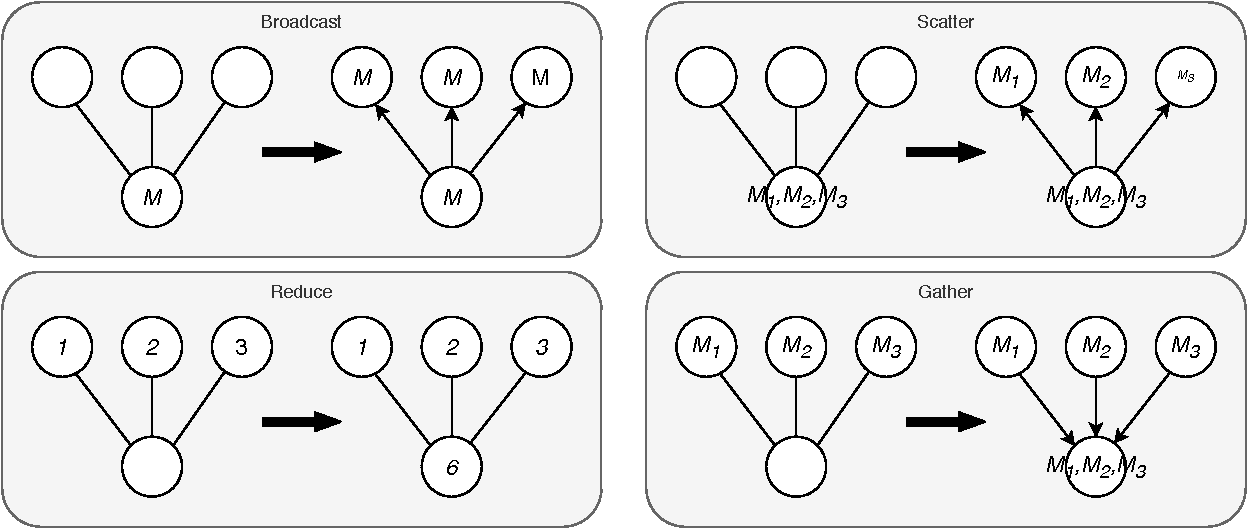
\includegraphics[width=1\textwidth]{./img/mpi_group_communication.pdf} 
	\caption{Schematische Darstellung der \emph{Broadcast}, \emph{Scatter}, \emph{Gather} und \emph{Reduce} Funktion in MPI}
	\label{fig:mpi_group_communication}
	% TODO Eventuell Pfeile bei reduce hinzufügen?
\end{figure}
\\ \noindent
Mit der \emph{Broadcast} Funktion kann ein Prozess eine Nachricht $M$ an alle anderen beteiligten Prozesse senden \cite{dongarra1995introduction}. Diese einfache Operation wird in vielen Fällen benötigt, wenn beispielsweise der \emph{Master} Prozess in einem Cluster Daten an alle \emph{Slaves} senden muss. Mit der \emph{Scatter} Funktion kann ein Prozess die Elemente einer Liste bzw. eines Arrays gleichmäßig an die anderen Prozesse verteilen, sodass jeder Empfänger nur einen Teil der Daten erhält \cite{nielsen2016introduction}. Diese Operation kann eingesetzt werden, wenn für jedes Element der Liste eine vom Rest unabhängige Berechnung durchgeführt werden muss. Zwar wäre es in einem solchen Szenario auch möglich, die \emph{Broadcast} Funktion zu verwenden und dann basierend auf dem Rang die Berechnung durchzuführen, aber bei der \emph{Scatter} Funktion werden insgesamt weniger Daten übertragen und somit eine geringere Bandbreite benötigt. Das Pendant zur \emph{Scatter} Funktion ist die \emph{Gather} Funktion. Hierbei erhält ein Prozess von allen anderen eine Nachricht $M_i$ und aggregiert diese in einer Liste oder einem Array \cite{nielsen2016introduction}. Die \emph{Scatter} und \emph{Gather} Funktionen werden häufig zusammen verwendet. Mit der \emph{Scatter} Funktion können die Daten an die verschiedenen Prozesse verteilt werden, diese berechnen ihre Ergebnisse, welche zuletzt mit der \emph{Gather} Funktion wieder gesammelt werden. Die letzte hier vorgestellte Funktion wird \emph{Reduce} genannt. Mit dieser können verschiedene globale Berechnungen mit einem binären kommutativen Operator durchgeführt werden \cite{nielsen2016introduction}. Eine Rechenoperation ist kommutativ, wenn für alle $a$ und $b$ einer Menge $M$  die Gleichung $a*b=b*a$ gilt \cite{walz2011brueckenkurs}. In Abbildung \ref{fig:mpi_group_communication} wird die Summe berechnet, aber \ac{MPI} bietet darüber hinaus andere Standardoperatoren, wie die Berechnung des Produkts, Minimums oder Maximums \cite{nielsen2016introduction}. 
\\\\
\ac{MPI} bietet noch weitere Arten der Gruppenkommunikation, auf welche an dieser Stelle nicht ausführlich eingegangen wird. Die \emph{AllGather} Funktion kombiniert die \emph{Gather} Funktion mit einem anschließenden \emph{Broadcast} des Ergebnisses. Bei der \emph{AllToAll} Funktion besitzt jeder Prozess eine Liste und sendet jeweils ein Element an jeden anderen Prozess \cite{dongarra1995introduction}. Eine spezielle Art der Gruppenkommunikation sind die sogenannten Synchronisationsbarrieren, an denen die Ausführung der einzelnen Prozesse angehalten wird, bis alle Teilnehmer diese erreicht haben \cite{nielsen2016introduction}. Abschließend sind zwei Anmerkungen zu nennen, welche für die verschiedenen Arten der Gruppenkommunikation wichtig sein können. Erstens ist jede dieser Operationen nur als synchrone Funktion verfügbar. Die zweite Anmerkung betrifft die Synchronisationsbarrieren. Bei vielen Implementierungen haben Funktionen wie der \emph{Broadcast} einen Synchronisationsseiteneffekt. Dies ist durch den \emph{MPI} Standard möglich, jedoch keine Voraussetzung und kann somit die Portierung von Projekten beeinflussen, die von diesen Seiteneffekten abhängig sind \cite{dongarra1995introduction}.

\subsection{Performance}
\label{subsec:basics_performance}
% Eventuell load balancing, wichtig
Das Erstellen eines gut parallelisierten Algorithmus ist häufig bedeutend schwieriger als das Erstellen desselben in einer sequenziellen Variante. Der Grund hierfür ist, dass zwar jeder parallele Algorithmus sequenziell ausführbar ist, indem die unabhängigen Teilaufgaben nacheinander abgearbeitet werden, dies aber umgekehrt nicht möglich ist. Um gute Ergebnisse zu erzielen, muss der parallelisierte Algorithmus häufig neu erstellt oder umstrukturiert werden. \cite{nielsen2016introduction}. Dieses Kapitel stellt Methoden vor, mit welchen die tatsächliche und maximal zu erwartende Performance eines parallelen Algorithmus berechnet werden kann. 
\\\\
Bevor auf die genauen Berechnungen eingegangen wird, sei angenommen, dass die serielle Ausführung eines Algorithmus $t_{seq}$ lange dauert und dass $t_q$ die Zeit angibt, welche derselbe parallele Algorithmus mit $P$ Prozessoren benötigt. Der sogenannte \emph{SpeedUp} gibt an, um welchen Faktor die parallele Ausführung eines Programms schneller ist. Berechnet wird dies mit $SpeedUp(P)=\frac{t_{seq}}{t_P}$ \cite{nielsen2016introduction}. Der \emph{SpeedUp} gibt nicht an, wie gut oder schlecht die tatsächliche Parallelisierung ist. Hierfür wird die Effizienz $e$ benötigt, welche mit $e=\frac{SpeedUp(P)}{P}$ berechnet wird. An dieser kann abgelesen werden, wie gut die parallele Ausführung tatsächlich ist. Der berechnete Wert liegt meistens zwischen $0$ und $1$, wobei ein niedriger Wert ein dafür Indiz ist, dass durch die Parallelisierung und eventuelle Kommunikation viel zusätzlicher Rechenaufwand entsteht. Dementsprechend zeigt ein hoher Wert, dass wenig zusätzlicher Aufwand entsteht und die Parallelisierung effizient erfolgt. In seltenen Fällen ist es sogar möglich, dass höhere Werte als $1$ erzielt werden, was einem \emph{super-linear SpeedUp} entspricht. Dies kann vorkommen, wenn beispielsweise mehrere Prozesse denselben \emph{Cache} verwenden. Hierbei ist es möglich, dass ein Prozess Rechenzeit einsparen kann, indem er ein Ergebnis aus dem \emph{Cache} wiederverwendet, das ein anderer Prozess berechnet hat \cite{nielsen2016introduction}.
\\\\
Mit den vorgestellten Formeln lassen sich der \emph{SpeedUp} und die Effizienz berechnen, sie geben allerdings keine Auskunft darüber, was der höchst mögliche \emph{SpeedUp} bzw. die kürzeste Ausführungszeit ist. Um diese zu berechnen, gibt es zwei Theoreme, welche unter den Begriffen \emph{Amdahl's Law} und \emph{Gustafson's Law} bekannt sind \cite{nielsen2016introduction}. 
\\\\
\emph{Amdahl's Law} wurde 1967 von Gene Amdahl in seiner Arbeit in Quelle \cite{amdahll1967validity} beschrieben. Die im Folgenden vorgestellten Formeln wurden erst später hieraus abgeleitet \cite{amdahll1967validity}. Angenommen wird ein Algorithmus bestehend aus zwei Teilen, bei dem der erste Teil $\alpha_{seq}$ rein sequenziell und der zweite Teil $\alpha_{par}$ parallelisierbar ist. Weiterhin wird angenommen, dass $\alpha_{seq}+\alpha_{par}=1$ ist und dass $t_1$ die Zeit angibt, welche ein einzelner Prozess zum Ausführen eines Programmabschnittes benötigt. Die Ausführungszeit $t_P$ eines solchen parallelisierten Programms mit $P$ Prozessen kann mit $t_P=\alpha_{seq} \cdot t_1 + \alpha_{par} \cdot \frac{t_1}{P}$ berechnet werden. Um den höchsten erreichbaren \emph{SpeedUp} zu berechnen wird angenommen, dass $t_1=t_{seq}$ gilt und der erhaltenen Wert $t_P$ in die bereits vorgestellte Formel für die Berechnung des \emph{SpeedUps} eingesetzt wird. Hierdurch ergibt sich die bekannte Formel von \emph{Amdahl's Law} \cite{nielsen2016introduction}: 
$$SpeedUp(P)=\frac{1}{\alpha_{seq}+\frac{\alpha_{par}}{P}}$$
Angenommen, es gäbe unendlich viele Prozessoren ($P \rightarrow \infty$), dann ist die Ausführungszeit des parallelisierbaren Programmteils vernachlässigbar gering, sodass nur der sequenzielle Anteil das Ergebnis maßgeblich beeinflusst und somit gilt \cite{nielsen2016introduction}:
$$\lim _{P \rightarrow \infty} SpeedUp(P)=\frac{1}{\alpha_{seq}}$$
Ist ein Algorithmus beispielsweise zu $95\%$ parallelisierbar und dementsprechend zu $5\%$ seriell, dann beträgt der maximale \emph{SpeedUp} für diesen $20$. \emph{Amdahl's Law} gilt unter der Annahme, dass bei steigender Prozessanzahl der Rechenaufwand der zu lösenden Aufgabe konstant bleibt, was auf viele Anwendungsszenarien zutrifft \cite{nielsen2016introduction}. Im Gegensatz hierzu steht das \emph{Gustafson's Law}, welches von John Gustafson stammt. Dieser argumentiert, dass \emph{Amdahl's Law} parallelen Systemen nicht gerecht würde, da der eigentliche Vorteil von diesen die Bearbeitung von größeren Datenmengen in derselben Zeit sei. In diesem Fall wird mit steigender Prozessanzahl ebenfalls der Rechenaufwand erhöht. Dies ermöglicht es, höhere \emph{SpeedUp} Werte zu erzielen \cite{hill2008amdahl}.





















% !TeX spellcheck = de_DE
\chapter{Softwarearchitektur und Implementierung}
\label{chap:software_architecture}
(TODO Anmerkung)
Das grundsätzliche Ziel ist, die in den Grundlagen vorgestellten Konzepte von den \ac{KNN}, neuroevolutionären Algorithmen, \ac{NEAT} und \ac{MPI} praktisch umzusetzen und für eine Anwendung zu kombinieren

% Warum python Etc
% Klassen übersicht, interface NN, interface NEAT, Service klassen, Challenge interface
Architektur und Implementierung, Aufbau, Klassen, Programmablauf
% !TeX spellcheck = de_DE
\section{Anforderungen}
\label{sec:requirements}
Aus dem Untertitel dieser Arbeit \emph{Analyse und Optimierung von \ac{NEAT} für ein verteiltes System} können drei verschiedene Ziele abgeleitet werden, mit welchen sich die folgenden Kapitel beschäftigten. Das erste Ziel ist die Implementierung einer sequentiellen Version des \ac{NEAT} Algorithmus. Hierauf basiert die zweite Phase, in welcher die korrekte Funktionalität der Implementierung verifiziert sowie eine Performance Analyse durchgeführt wird. 
Basierend auf der Analyse ist das dritte Ziel die Optimierung des Algorithmus mit \ac{MPI} für einen Bewoulf Cluster
\\\\
Dieses Kapitel befasst sich mit dem ersten Ziel, der Implementierung des sequenziellen Algorithmus. Hierzu werden in einem ersten Schritt verschiedene Anforderungen an die Software definiert, welche sowohl von der sequenziellen als auch der später vorgestellten parallelisierten Implementierung erfüllt werden müssen. Danach wird auf die verschiedenen Datenstrukturen, Schnittstellen und Implementierungsdetails eingegangen.
\\\\
Die erste Anforderung betrifft die Programmiersprache. Für dieses Projekt soll die Sprache Python verwendet werden. Dies ist eine moderne, einfach zu lernende Hochsprache, deren Vorteile eine einfache Syntax sowie die dynamische Typisierung von Variablen und Parametern sind. Dies ermöglicht in vielen Fällen eine schnelle Entwicklung von Prototypen oder auch vollwertigen Softwaresystemen. Zusätzlich bietet die Sprache viele verschiedene \emph{open source} Pakete, welche einfach in bestehende Projekte integriert werden können und fertige Lösungen für diverse Aufgabengebiete bieten. Aus diesem Grund ist Python eine der bekanntesten Sprachen im Bereich Forschung und Entwicklung \cite{dalcin2011parallel}. Dies gilt insbesondere für die Bereiche \emph{Machine Learning} und \ac{KNN}, da viele hierfür verwendete Bibliotheken primär für Python entwickelt sind, wie beispielsweise Tensorflow \cite{tensorflow2015}, Pytorch \cite{pytorch2019} und das OpenAI Gym \cite{OpenAiGym2016}. Letzteres ist eine Bibliothek, welche verschiedene Testumgebungen für das bestärkende Lernen bietet und welche auch in dieser Arbeit eingesetzt wird.  
\\\\
Die nächste Anforderung betrifft das Projekt selbst. Dieses soll wie eine Bibliothek eingesetzt werden können und muss somit eine einfache Programmierschnittstelle für den Anwender bieten. Das Ziel ist, dass mit wenig Aufwand verschiedene Optimierungsprobleme umgesetzt und gelöst werden können. Dies soll sowohl für Testumgebungen aus dem OpenAI Gym als auch für andere Quellen gelten. 
\\\\ % kapitel REF
Eine weitere wichtige Anforderung ist, dass der ganze Optimierungsprozess mithilfe eines \emph{Seeds} beeinflussbar und somit wiederholbar sein muss. Der Grund hierfür ist, dass wie in Kapitel \ref{sec:evolutionary_algos} und Kapitel \ref{sec:neat} aufgezeigt, neuroevolutionäre Algorithmen viele Zufallswerte verwenden, die den Ablauf und das erhaltene Ergebnis stark beeinflussen können. Für einen einfachen Vergleich zwischen der sequentiellen und parallelisierten Implementierung ist es notwendig, dass beide Algorithmen exakt denselben Ablauf an Instruktionen und dieselben Zufallswerte haben und somit letztendlich auch dieselbe Lösung liefern. Dies ist für einen sequenziellen Algorithmus einfach umzusetzen, wenn ein globaler Zufallsgenerator mithilfe eines \emph{Seeds} verwendet wird. Bei der Verwendung eines Beowulf Clusters ist dies nicht möglich, da hierbei physisch getrennte Geräte verwendet werden. Somit ist die Herausforderung, dass sowohl der sequenzielle als auch der parallelisierte Algorithmus unabhängig von der Anzahl an verwendeten Geräten unter Verwendung desselben \emph{Seeds} dieselben Lösungen berechnen.
\\\\
Zwei weitere wichtige Anforderungen betreffen die Performance und Visualisierung. Sowohl in der sequenziellen als auch der parallelisierten Implementierung muss es möglich sein, die benötigte Ausführungszeit zu messen. Die hierbei erhaltenen Ergebnisse sind die Grundlage für den späteren Performance Vergleich. Zusätzlich sollen die erfassten Werte in entsprechenden Diagrammen visualisiert werden können. Neben den Zeiten sollen auch die durch \ac{NEAT} erzielten Ergebnisse dargestellt werden. Dies umfasst unter anderem die Struktur der optimierten \ac{KNN}, die erreichten Fitnesswerte, die Verteilung der Spezies (TODO Eventuell weg?) und in einigen Fällen auch die Lösungsstrategie. Letzteres bezieht sich vor allem auch auf das OpenAI Gym. Die Testumgebungen von diesem können in vielen Anwendungsfällen gerendert werden, was allerdings die Laufzeit enorm erhöht. Deswegen ist es bei dem eigentlichen Optimierungsprozess üblich, hierauf zu verzichten. Das letzte Ziel bezüglich der Visualisierung ist, dass ein gespeichertes Genom nach einem Trainingsverfahren geladen werden kann, hieraus ein \ac{KNN} gebildet wird und die Interaktion von diesem in der Testumgebung gerendert wird. Hierdurch ist es möglich, die entwickelten Strategien und Fortschritte nachzuverfolgen, ohne die Trainingszeit zu erhöhen.
\\\\
Hieraus ergibt sich auch die letzte Anforderung, die persistente Speicherung der Ergebnisse. Es soll möglich sein, die Genome, Fitnesswerte und gemessenen Laufzeiten persistent in einer Datei abzuspeichern. Die Speicherung der Genome ist Voraussetzung, dass diese visualisiert oder auch in einer Produktivumgebung eingesetzt werden können. Bezüglich der Fitnesswerte und Laufzeiten wäre es theoretisch möglich, die erstellten Graphen als Bilddatei oder Ähnliches zu speichern. Dies hat den Nachteil, dass die Werte nicht automatisiert ausgelesen werden können und ein genauer Vergleich mit anderen Datensätzen schwierig ist. Aus diesem Grund sollen in dieser Arbeit die Rohdaten gespeichert werden, sodass auch eine nachträgliche Verarbeitung beziehungsweise ein Vergleich mit anderen Durchläufen möglich ist. Neben der generellen Speicherung der finalen Ergebnisse soll auch eine regelmäßige Zwischenspeicherung möglich sein, zum Beispiel nach jeder Generation. Der Grund hierfür ist \ac{MPI}. In Kapitel \ref{subsubsec:mpi_and_mapreduce} ist erläutert, dass dieses beim Auftreten von Fehlern die Ausführung komplett abbricht und nicht gespeicherte Ergebnisse verloren gehen. Durch die Speicherung der Zwischenergebnisse entsteht kein Datenverlust und somit auch keine Verschwendung der bisher genutzten Rechenzeit.



% !TeX spellcheck = de_DE
\section{Softwarearchitektur}
\label{sec:software_architecture}
Im Folgenden wird auf die Architektur der Software sowie der Implementierung des sequenziellen Verfahrens eingegangen. Das grundsätzliche Ziel ist, dass so viele Komponenten wie möglich von der sequentiellen und parallelisierten Implementierung genutzt werden können, sodass einerseits der programmiertechnische Aufwand möglichst gering ist und andererseits ein einfaches Austauschen der beiden Varianten möglich ist. Hierfür wird eine Kombination aus verschiedenen Interfaces sowie Serviceklassen verwendet, auf welche im Rahmen dieses Kapitels genauer eingegangen wird. Zuvor werden noch die verwendeten Datenstrukturen und das Interface für die Bibliothek vorgestellt.
 
\subsubsection{Datenstrukturen}
\label{subsubsec:data_structures}
Die verwendeten Datenstrukturen sind für beide Implementierungen identisch und in Abbildung (TODO ABBILDUNG) in einem UML Diagramm dargestellt. Wie zu erkennen ist, besitzen diese keine Funktionen und können so für beide Implementierungen genutzt werden. Die eigentliche Funktionalität wird in den später vorgestellten Serviceklassen umgesetzt.
\\\\
Die erste Struktur ist das \emph{Genom}, welches aus Kapitel \ref{sec:neat} bekannt ist und alle Informationen zur Konstruktion eines \ac{KNN} besitzt. Hierfür werden zwei Listen benötigt, wobei die erste alle Neuronen und die zweite alle Verbindungen des \ac{KNN} enthält. Diese Repräsentation entspricht der Kodierung aus Kapitel \ref{subsec:neat_encoding}. 
\\\\
Ein Neuron wird durch die Klasse \emph{Node} repräsentiert und enthält unter anderem den Bias-Wert und die zu verwendende Aktivierungsfunktion, welche für die Berechnungen im \ac{KNN} benötigt werden. Zusätzlich sind einige weitere Werte vorhanden, welche die spätere Implementierung der Anforderungen vereinfachen. Hierzu gehört unter anderem der Neuronentyp, welcher angibt, ob es sich um ein \emph{Input}-, \emph{Hidden}- oder \emph{Ouput}-Neuron handelt. Dies vereinfacht die spätere Visualisierung sowie das Einsetzen der Eingabewerte und das Auslesen des Ausgabevektors. Zusätzlich besitzt jedes Neuron eine X-Koordinate, welche die relative X-Position für eine spätere Visualisierung angibt. Die \emph{Input}- und \emph{Output}-Neuronen besitzen die Werte $0$ und $1$. Die \emph{Hidden}-Neuronen werden, wie in Kapitel \ref{subsec:neat_minimal_structure} beschrieben, nur durch strukturelle Mutationen hinzugefügt und dabei zwischen zwei anderen Neuronen platziert. Die X-Koordinate von diesen wird berechnet, indem der Mittelwert der zwei anderen Neuronen gebildet wird. Zuletzt enthält jedes Neuron zur Identifizierung eine ID, welche von den Verbindungen genutzt wird.
\\\\
Eine Verbindung zwischen zwei Neuronen wird im Genom durch eine Instanz der Klasse \emph{Connection} repräsentiert. Jede von diesen enthält zwei Werte, welche die ID des Start- und Zielneurons der Verbindung enthalten. Zusätzlich ist das Gewicht sowie ein Aktivierungsbit gegeben. Letzteres gibt entsprechend der vorgestellten Kodierung an, ob die Verbindung im \ac{KNN} enthalten sein soll. Die letzte Variable ist die Innovationsnummer, welche in Kapitel \ref{subsec:neat_reproduction} beschrieben ist. Diese wird durch strukturelle Mutationen zugewiesen und in der Reproduktionsphase zum Lösen des \emph{Competing Conventions} Problems verwendet.
\\\\
In Kapitel \ref{sec:evolutionary_algos} ist der Begriff des Individuums erläutert. In dieser Arbeit werden diese durch Instanzen der Klasse \emph{Agent} repräsentiert und sind nach dem Agenten benannt, welcher beim bestärkenden Lernen mit der Umwelt interagiert. Der hierbei erhaltene Fitnesswert, welcher im späteren Verlauf die Selektion maßgeblich beeinflusst, wird in der entsprechenden Variable \emph{fitness} gespeichert. Das Feld \emph{additional\_info} kann Zusatzinformationen enthalten, welche vom Optimierungsproblem stammen können.
\\\\
Die zwei letzten Klassen in diesem Diagramm sind die \emph{Generation} und \emph{Spezies}. Letzteres ist aus dem \ac{NEAT} Kapitel bekannt und ist eine Gruppierung von ähnlichen Individuen bzw. Agenten. Entsprechend der in Kapitel \ref{subsec:neat_species} enthaltenen Definition ist eine Spezies durch ein Genom repräsentiert und besitzt eine Mitgliederliste. Zusätzlich wird der höchste erreichte Fitnesswert des besten Mitglieds gespeichert sowie die Generation, in welcher dieser Wert erzielt wurde. Dies wird benötigt, um den Fortschritt zu überwachen, da eine Spezies nicht für die Reproduktion ausgewählt wird, deren Mitglieder keine Steigerung des Fitnesswertes in einer festgelegten Anzahl an Generationen erzielen.
\\\\
Die letzte Klasse ist die \emph{Generation}, welche aus Kapitel \ref{subsec:evolutionary_algorithm} bekannt ist. Diese enthält sowohl eine Liste mit allen Individuen als auch eine der verschiedenen Spezies. Zusätzlich wird diese durch eine Nummer identifiziert, welche angibt, wie viele Zyklen der Evaluation, Selektion, Rekombination und Mutation bereits durchgeführt wurden.

\subsubsection{Künstliches neuronales Netz}
Aus dem Genom wird ein \ac{KNN} erstellt, welches dann im Optimierungsproblem eingesetzt wird. In Kapitel \ref{sec:neuroal_networks} sind der Aufbau und die Funktionsweise von diesen ausführlich erläutert. Prinzipiell können hierfür verschiedene bereits implementierte Bibliotheken verwendet werden, wie beispielsweise Tensorflow \cite{tensorflow2015} oder PyTorch \cite{pytorch2019}. Mit diesen können vor allem rein ebenenweise verbundene \ac{KNN}, wie in Kapitel \ref{subsec:network_structures} vorgestellt, schnell und einfach erstellt werden. Allerdings können durch \ac{NEAT} auch \ac{KNN} mit \emph{shortcut} Verbindungen entstehen sowie Netze mit Rückkopplungen. Zwar können diese  auch mit Tensorflow und PyTorch abgebildet werden, aber dies erfordert einen bedeutend höheren Aufwand. Da dies im Rahmen dieser Arbeit nicht möglich ist, wird eine eigene vereinfachte Implementierung verwendet. Ein Nachteil von dieser ist, dass sie im Vergleich zu Implementierungen aus großen Bibliotheken insgesamt langsamer ist. Der Grund hierfür ist, dass die Bibliotheken gut optimiert sind und auch die Verwendung von \acp{GPU} unterstützen, welche die benötigte Ausführungszeit stark reduzieren können. Auch wenn diese nicht verwendet werden, wird im Folgenden ein Grundgerüst erstellt, sodass eine spätere Integration einfach möglich ist. Dies wird mit einem Interface realisiert, welches die grundlegenden Funktionen definiert. Sowohl die in dieser Arbeit verwendete Implementierung als auch zukünftige Erweiterungen mit Tensorflow oder ähnlichem können dieses nutzen und ermöglichen somit ein einfaches Austauschen der verschiedenen Implementierungen. Das Interface ist in Abbildung (TODO ABBILDUNG) dargestellt und definiert drei Funktionen mit den Namen \emph{build()}, \emph{reset()} und \emph{activate()}. Bei der \emph{build()} Funktion wird ein Genom übergeben und hieraus ein \ac{KNN} konstruiert. Die \emph{activate()} Funktion bekommt eine Liste mit Eingabewerte übergeben und produziert den Ausgabevektor des \ac{KNN}. Die Anzahl an Eingabe- und Ausgabewerten entspricht der Anzahl an \emph{Input}- und \emph{Output}-Neuronen im \ac{KNN}. Bei der \emph{reset()} Funktion werden eventuell gespeicherte Ergebnisse, wie sie bei einem Netz mit Rückkopplungen enthalten sein können, entfernt und auf den Startwert zurückgesetzt. 
\\\\
Die in dieser Arbeit verwendete \emph{BasicNeuralNetwork} Implementierung setzt dieses Interface mit dem Ziel um, dass sowohl Netze mit und ohne Rückkopplungen umgesetzt werden können. Da eine genaue Beschreibung der Implementierung nicht von Interesse ist, wird an dieser Stelle nur der oberflächliche Ablauf beschrieben. Bei der \emph{build()} Funktion wird je eine Liste für die \emph{Input}- und \emph{Output}-Neuronen angelegt, in welche die Neuronen mit den entsprechenden Typen sortiert werden. Eine dritte Liste enthält alle im \ac{KNN} enthaltenen Neuronen. Jedes Neuron speichert zudem eine Liste mit den Verbindungen, welche zu ihm führen und den aktuellen sowie letzten berechneten Wert. Die letzte Aufgabe dieser Funktion ist die Festlegung der Reihenfolge, in welcher die einzelnen Neuronen aktiviert bzw. deren Zwischenergebnisse berechnet werden. Bei der Reihenfolge ist zu beachten, dass bei einem Netz ohne Rückkopplung jedes vorherige Neuron bis zu den \emph{Input-Neuronen} bereits aktiviert sein muss, da ansonsten das Ergebnis verfälscht wird. Bei Netzen mit Rückkopplungen gilt diese Anforderung prinzipiell auch, außer für Verbindungen, welche in derselben Schicht oder von Neuronen der nachfolgenden Schichten ausgehen. Dies sind Rückkopplungen, bei welchen der zuletzt berechnete Wert zurückgeben wird, sodass keine Endlosschleife entsteht. 
\\\\
Bei der \emph{activate()} Funktion wird ein Eingabevektor an das \ac{KNN} übergeben. Jeder darin enthaltene Wert wird in ein \emph{Input}-Neuron gesetzt. Dies ist mit der zuvor in der \emph{build()} Funktion erstellten Liste mit allen \emph{Input}-Neuronen effizient umzusetzen. Danach beginnt die eigentliche Berechnung des Ausgabevektors. Hierzu werden die Neuronen in der zuvor festgelegten Reihenfolge aktiviert bzw. berechnet. Zuletzt wird der Ausgabevektor erstellt. Auch dies ist effizient umsetzbar, da zuvor ein Liste mit allen \emph{Output}-Neuronen erstellt wurde. Über diese wird iteriert und die entsprechenden Ergebnisse in eine neue Liste kopiert, welche schlussendlich den Ausgabevektor repräsentiert und als Ergebnis der Funktion zurückgegeben wird. 
\\\\
Die \emph{reset()} Funktion iteriert über die Liste mit allen Neuronen und entfernt die gespeicherten Zwischenergebnisse. 

\subsubsection{Optimierungsproblem}
In den vorherigen Kapiteln sind die grundlegenden Datenstrukturen und die Funktionalität des \ac{KNN} vorgestellt. Bevor der eigentliche Optimierungsalgorithmus implementiert werden kann, wird noch eine grundlegende Komponente benötigt und zwar das Optimierungsproblem. Wie in Kapitel \ref{subsub:optimzation_problem} vorgestellt, können diese aus verschiedenen Domänen stammen und sich sehr unterscheiden. Somit muss auch für dieses ein Interface mit dem Ziel erstellt werden, möglichst viele Szenarien abbilden zu können, welche einfach und mit wenig Aufwand durch das in dieser Arbeit implementierte Verfahren optimierbar sind.
\\\\
Das Interface ist in Abbildung (TODO ABBILDUNG) dargestellt und zeigt fünf Funktionen, von welchen lediglich die \emph{evaluate()} Funktion immer benötigt wird. Die restlichen vier Funktionen sind optional und können je nach Optimierungsproblem zusätzlich eingesetzt werden. Im Folgenden wird auf die Bedeutung von diesen genauer eingegangen.
\\\\
Die \emph{initialization()} Funktion kann zum Initialisieren der Umgebung verwendet werden und wird einmalig zu Beginn durch die später vorgestellte Bibliothek aufgerufen. Dies kann beispielsweise verwendet werden, um notwendige Daten initial aus einer Datenbank zu laden oder um die Umgebung zu erstellen. Ist die Initialisierung abgeschlossen, können prinzipiell verschiedene Agenten in dieser evaluiert werden. Vor jeder Evaluation wird die \emph{ before\_evaluation()} Funktion aufgerufen, mit welcher zum Beispiel der Zustand der Umgebung zurückgesetzt werden kann, sodass jeder Agent denselben Startzustand vorfindet. Danach wird die eigentliche Evaluation mit der Funktion \emph{evaluate()} durchgeführt. Dies ist die wichtigste Funktion in diesem Interface und muss von jedem Optimierungsproblem implementiert werden. Als Parameter wird ein initialisiertes \ac{KNN} übergeben, welches mit dem Genom eines Agenten erstellt wurde. Mit diesem soll das Optimierungsproblem gelöst werden. Die genaue Implementierung dieser Funktion kann je nach Problem sehr unterschiedlich sein. Verschiedene Beispiele werden in Kapitel \ref{chap:analysis} genauer vorgestellt. Bei der Implementierung ist zu beachten, dass die Funktion zwei Rückgabewerte erwartet. Der erste ist vom Typ \emph{float} und repräsentiert den erreichten Fitnesswert. Wie in Kapitel \ref{subsub:optimzation_problem} vorgestellt, bewertet dieser die Leistung des \ac{KNN} und wird für die spätere Selektionsphase benötigt. Der zweite Rückgabewert ist vom Typ \emph{Dict} und kann verschiedene \emph{Key-Value} Paare mit Zusatzinformationen des Optimierungsproblems enthalten. Diese werden letztendlich im Datenfeld \emph{additional\_info} des Agenten gespeichert, welches in Kapitel \ref{subsubsec:data_structures} vorgestellt ist. Die darin gespeicherten Daten können für eine spätere Auswertung sowie in der Abbruchbedingung für den Algorithmus verwendet werden. Nach jeder durchgeführten Evaluation wird das Pendant zur \emph{before\_evaluation()} Funktion ausführt, dies ist die \emph{after\_evaluation()} Funktion. Mit dieser sowie der letzten in diesem Interface enthaltenen Funktion \emph{clean\_up()} können verschiedene Tätigkeiten umgesetzt werden, welche Ressourcen freigeben oder den originalen Zustand der Umgebung wiederherstellten. Der Unterschied zwischen diesen Funktionen ist, dass die \emph{clean\_up()} Funktion das Pendant zur \emph{initialization()} Funktion ist und nur einmalig am Ende des Trainingsverfahren aufgerufen wird. 
 
\subsubsection{Schnittstelle der Bibliothek}
\label{subsubsec:library_interface}
Nachdem die für diese Arbeit benötigten Komponenten vorgestellt sind, kann auf die Schnittstelle der Bibliothek genauer eingegangen werden. Ziel ist, dass diese die grundlegenden Funktionen definiert, welche sowohl von der sequentiellen als auch der parallelisierten Implementierung umgesetzt werden. Somit bieten beide Implementierungen dieselben Funktionalitäten, können einfach ausgetauscht werden und ermöglichen einen einfachen Vergleich. 
\\\\
Die Schnittstelle der Bibliothek besteht aus drei Interfaces, die als \emph{NeatOptimizer}, \emph{NeatReporter} und \emph{NeatOptimizerCallback} bezeichnet werden und deren Beziehung zueinander in Abbildung (TODO ABBILDUNG) dargestellt ist. Zu erkennen ist, dass der \emph{NeatOptimizerCallback} von dem \emph{NeatReporter} erbt und somit dessen Funktionalität erweitert. Der \emph{NeatOptimizer} besitzt genau einen \emph{NeatOptimizerCallback} sowie beliebig viele \emph{NeatReporter}. Auf die Funktionalität von diesen wird später genauer eingegangen. Im Folgenden wird zuerst der \emph{NeatOptimizer} betrachtet, welcher fünf Funktionen besitzt, von denen vier für das Hinzufügen und Entfernen von Instanzen der Klasse \emph{NeatReporter} und \emph{NeatOptimizerCallback} verwendet werden. Die letzte Funktion hat den Namen \emph{evaluate()}, startet den Ablauf des Optimierungsproblems und erhält als Parameter die hierfür benötigten Werte. Die ersten beiden Parameter bestimmen die Anzahl der \emph{Input}- und \emph{Output}-Neuronen und somit die Größe des Eingabe- und Ausgabevektors. Da der Optimierungsvorgang in \ac{NEAT}, wie in Kapitel \ref{subsec:neat_minimal_structure}  beschrieben, mit einer minimalen Struktur beginnt, müssen keine \emph{Hidden}-Neuronen angegeben werden. Der nächste Parameter ist eine Referenz auf eine Aktivierungsfunktion, welche von allen Neuronen verwendet wird. Einige bekannte Vertreter, von denen ein Teil in Kapitel \ref{subsubsec:activatoin_function} vorgestellt ist, sind standardmäßig in diesem Projekt enthalten, wobei das Hinzufügen von weiteren Funktionen jederzeit möglich ist. Hierauf folgt der Parameter \emph{challenge}, der eine Klasse repräsentiert, die das Interface des Optimierungsproblems implementiert. Der Algorithmus wird versuchen, das hierin enthaltene Problem zu optimieren. Die letzten beiden Parameter sind als \emph{config} und \emph{seed} bezeichnet. Letzteres soll die Generierung der Zufallswerte beeinflussen und somit den Optimierungsvorgang wiederholbar und vergleichbar machen. Die \emph{config} repräsentiert eine Konfiguration, in welcher verschiedene Parameter des Verfahrens spezifiziert sind. In dieser wird beispielsweise angegeben, wie hoch die Chance auf eine strukturelle Mutation ist oder wie sehr sich die Gewichte der Verbindungen ändern können. Auf die tatsächlich verwendeten Konfigurationen wird im Rahmen der Analyse in Kapitel \ref{chap:analysis} weiter eingegangen.
\\\\
Das Ausführen der \emph{evaluate()} Funktion startet den gesamten Optimierungsprozess, welcher je nach Komplexität eine Laufzeit von mehreren Stunden oder Tagen haben kann. Häufig ist es in diesen Anwendungsfällen gewünscht, Zwischenergebnisse und Fortschritte anzuzeigen, sodass die verbleibende Laufzeit und der Erfolg des Verfahrens besser abschätzbar ist. Dies wird in dieser Arbeit durch Callbacks realisiert, welche durch die Interfaces \emph{NeatReporter} und \emph{NeatOptimizerCallback} implementiert werden. Das Interface \emph{NeatReporter} definiert einige Methoden, welche während der Laufzeit des Algorithmus regelmäßig an bestimmen Punkten aufgerufen werden. Klassen, die diese implementieren, können hierdurch Statusinformationen über den aktuellen Zustand sowie den Fortschritt des Verfahrens erhalten. 
Dieses Interface wird in dieser Arbeit unter anderem für die regelmäßige Speicherung des besten Agenten und zur Messung der Performance genutzt. Die erste hierbei implementierte Funktion ist die \emph{on\_initialization()}, welche einmalig zu Beginn aufgerufen wird. Das Pendant hierzu ist die \emph{on\_cleanup()} Funktion, welche einmalig am Ende aufgerufen wird. Auch für die Zwischenzeit gibt es einige Methoden, die den Beginn und das Ende verschiedener Phasen signalisieren. Die Funktionen \emph{on\_generation\_evaluation\_start()} und \emph{on\_generation\_evaluation\_end()} werden zum Beginn und Ende der Evaluationsphase aufgerufen. Als Parameter wird an beide Funktionen die aktuell evaluierte Generation übergeben. Dies kann beispielsweise zum Nachverfolgen des besten und durchschnittlichen Fitnesswertes verwendet werden. Mit den Funktionen \emph{on\_agent\_evaluation\_start()} und \emph{on\_agent\_evaluation\_endt()} wird angegeben, wann die Evaluierung eines einzelnen Agenten beginnt und abgeschlossen ist. An diese Funktion wird der eigentliche Agent sowie ein Index übergeben, welcher angibt, wie viele Evaluationen in dieser Generation bereits durchgeführt wurden. Diese Informationen können beispielsweise für einen Fortschrittsbalken verwendet werden. Die Funktionen \emph{on\_reproduction\_start()} und \emph{on\_reproduction\_end()} markieren den Beginn und das Ende der Reproduktionsphase, welche mit der Selektion startet und mit dem Ersetzen der vorherigen Generation durch die neu erstellten Agenten endet. Um die Zeit zu messen, welche für die Rekombination und Mutation eines einzelnen neuen Agenten benötigt wird, sind die Funktionen \emph{on\_compose\_offsprings\_start()} und  \emph{on\_compose\_offsprings\_end()} enthalten. Die letzte in diesem Interface enthaltene Funktion heißt \emph{on\_finish()} und erhält als Parameter die aktuelle Generation. Sie wird einmalig am Ende der Optimierung aufgerufen nachdem die Abbruchbedingung erfüllt ist. Diese kann verwendet werden, um das beste \ac{KNN} und die erhaltenen Ergebnisse zu visualisieren und zu speichern.
\\\\
Die Klasse \emph{NeatOptimizerCallback} erbt von dem Interface \emph{NeatReporter} und kann daher alle bereits vorgestellten Funktionen nutzen. Diese sind für den Programmablauf optional und werden nicht zwingend benötigt. Dies trifft nicht auf die letzte Funktion zu, welche im \emph{NeatOptimizerCallback} zusätzlich implementiert wird. Dies ist die Funktion \emph{finish\_evaluation()}, welche die aktuelle Generation als Parameter übergeben bekommt und einen Wert vom Typ \emph{boolean} zurückgeben muss. Hiermit wird die Abbruchbedingung umgesetzt. Die Funktion wird nach Beendigung der Evaluationsphase mit der aktuellen Generation sowie mit allen erzielten Fitnesswerten aufgerufen. Ist das Ergebnis der Funktion \emph{True}, wird die Ausführung des Algorithmus beendet und die entsprechenden Callback Funktionen \emph{on\_finish()} und \emph{on\_cleanup()} aufgerufen. Liefert die Funktion \emph{False}, wird mit der Selektion, Rekombination und Mutation fortgefahren und der Zyklus startet erneut. Diese Art der Abbruchbedingung ermöglicht vielfältige Umsetzungen. Zum Beispiel kann der Algorithmus beendet werden, wenn der Fitnesswert eines Agenten einen Schwellwert übersteigt, eine gewisse Anzahl an Zyklen bzw. Generationen durchgeführt ist oder eine festgelegte Trainingszeit überschritten ist.

\subsubsection{Serviceklassen}
Ein wichtiges Ziel bei der Entwicklung ist das Einsparen von unnötigem Implementierungsaufwand, dies gilt auch für diese Arbeit. Aus diesem Grund wurden die bereits vorgestellten Interfaces erstellt, welche sowohl von der sequenziellen als auch der parallelisierten Implementierung verwendet werden. Der Vorteil hierdurch ist, dass ein einfaches Austauschen der beiden Umsetzungen möglich ist und einen einfachen Vergleich ermöglicht. Die eigentliche Implementierung wird sich zwangsläufig an einigen Punkten unterscheiden. Dennoch wird ein großer Teil der \ac{NEAT} Komponenten gleich bleiben, da sich die Funktionen nicht durch eine Parallelisierung ändern. Aus diesem Grund wird ein Großteil dieser Funktionen als Serviceklassen implementiert, die keinen internen Zustand besitzen und somit zwei Vorteile bieten. Erstens ist es einfach möglich, die Funktionen in verschiedenen Implementierungen zu nutzen. Zweitens ermöglicht eine solche Struktur ein einfaches automatisiertes Testen der Implementierung. Dies ist besonders wichtig, da Fehler im Trainingsverfahren zu einem späteren Zeitpunkt aufgrund der Größe der Population schwer zu lokalisieren sind.
\\\\
Insgesamt werden drei Serviceklassen mit den Namen \emph{GenerationService}, \emph{ReproductionService} und \emph{SpeciesService} erstellt, welche Funktionen entsprechend ihrer Benennung übernehmen. Somit befasst sich die erste Klasse mit allen Funktionen, welche die ganze Generation betreffen, die zweite mit Funktionen bezüglich dem Erstellen und Modifizieren von Genomen sowie Agenten und die letzte Klasse mit Funktionen bezüglich der verschiedenen Spezies. Im Folgenden wird auf die enthaltenen Funktionen jeder Serviceklasse genauer eingegangen. Allerdings sei hierzu angemerkt, dass keine genauen Implementierungsdetails vorgestellt werden. Die theoretische Funktionalität ist in den Kapiteln \ref{sec:evolutionary_algos} und  \ref{sec:neat} erläutert. Für die genaue praktische Umsetzung wird auf den veröffentlichten Programmcode verwiesen.
\\\\
Der \emph{ReproductionService} besitzt vor allem Funktionen, um neue Genome mittels Reproduktion zu erzeugen oder bestehende zu mutieren. Die erste Funktion heißt \emph{cross\_over()} und setzt die eigentliche Reproduktion um. In ihr werden zwei Elterngenome verwendet, um einen Nachkommen zu erzeugen. Grundsätzlich entsprechen sowohl die Umsetzungen dieser Funktion als auch der anderen in diesem Kapitel vorgestellten Funktionen den Erläuterungen der vorherigen Kapitel. Eine Besonderheit soll an dieser Stelle hervorgehoben werden. Ein wichtiges Ziel für ein wiederholbares Ergebnis ist, dass unabhängig von einem Prozessor mit demselben Seed immer dasselbe Ergebnis erzielt wird. Dies ist mit einem einfachen globalen Zufallsgenerator in einem verteilten System nicht möglich. Aus diesem Grund wird für jedes Genom ein neuer Zufallsgenerator erzeugt, dessen Seed sich aus den beiden Elterngenomen ergibt und welcher für alle Zufallsoperationen verwendet wird, die dieses Genom betreffen. Der hieraus resultierende Vorteil ist, dass unabhängig vom Prozessor und dessen internem Zustand dieselben Eltern immer denselben Nachkommen produzieren. Der hierfür erstellte Zufallsgenerator wird auch für die Funktionen \emph{mutate\_weights()}, \emph{mutate\_add\_connection()} und \emph{mutate\_add\_node()} verwendet. Die erste Funktion mutiert die Gewichte aller Verbindungen, die zweite fügt eine neue Verbindung und die dritte ein neues Neuron dem Genom hinzu. Bei letzterem werden entsprechend der Definition in Kapitel \ref{subsec:neat_mutation} zusätzlich zwei neue Verbindungen erstellt.
\\\\
Die Klasse \emph{GenerationService} besitzt einige Funktionen zum Erzeugen der initialen Population. Wie bei der Schnittstellendefinition beschrieben, wird anfänglich nur die Anzahl an \emph{Input}- und \emph{Output}-Neuronen übergeben. Die Funktion \emph{create\_genome\_structure()} erzeugt mit diesen Informationen eine Struktur für das \ac{KNN}, welche die entsprechenden Neuronen und Verbindungen enthält. In der Funktion \emph{create\_initial\_generation()} kann mit der generierten Struktur letztendlich eine neue Generation erstellt werden. Hierfür wird das Genom für jeden zu erstellenden Agenten einmal kopiert und die Gewichte der Verbindungen zufällig gesetzt. Schlussendlich werden die Agenten noch den Spezies zugeordnet.
\\\\
Der \emph{SpeciesService} besitzt im Vergleich zum \emph{GenerationService} bedeutend mehr Funktionen. Um die erstellten Agenten den verschiedenen Spezies zuzuordnen, kann die Funktion \emph{ sort\_agents\_into\_species()} genutzt werden. Entsprechend der Erläuterung in Kapitel \ref{subsec:neat_species} iteriert diese über die Liste mit allen Agenten und überprüft für jeden die Kompatibilität mit den existierenden Spezies. Der Kompatibilitätswert zwischen zwei Genomen kann mit der Funktion \emph{calculate\_genetic\_distance()} berechnet werden. Ist dieser kleiner als ein konfigurierter Schwellwert, wird der Agent der Spezies zugeordnet. Existiert keine passende Spezies, wird eine neue erstellt. Dies sind aber nicht die einzigen Funktionen. In Kapitel \ref{subsec:neat_species} ist das \emph{explicit fitness sharing} Verfahren eingeführt worden, welches mit der Funktion \emph{calculate\_adjusted\_fitness()} umgesetzt ist. Der angepasste Fitnesswert wird schließlich bei der Selektion verwendet, welche mit den Funktionen \emph{calculate\_amount\_offspring()} und \emph{create\_offspring\_pairs()} umgesetzt ist. Die erste Funktion berechnet, wie viele Nachkommen jede Spezies erhalten soll. Die zweite Funktion erstellt die tatsächlichen Elternpaare, welche zum Erzeugen der Nachkommen verwendet werden. Zuletzt sind noch einige kleinere Funktionen enthalten. Bei \ac{NEAT} können nur die besten $50\%$ der Genome zur Reproduktion ausgewählt werden, die Funktion \emph{remove\_low\_genomes()} entfernt die restlichen. Beim \ac{NEAT} Algorithmus wird nach jeder Generation ein neues Genom zum Repräsentieren jeder Spezies ausgewählt.  Dies ist in diesem Projekt mit der Funktion \emph{select\_new\_representative()} möglich. Die letzten beiden Funktionen heißen \emph{reset\_species()} und \emph{get\_species\_with\_members()}. Die erste hiervon entfernt alle Mitglieder einer Spezies. Dies wird typischerweise durchgeführt bevor die neu erstellten Agenten den Spezies zugewiesen werden. Nach der Zuweisung wird die zweite Funktion aufgerufen. Diese filtert Spezies heraus, welche keine Mitglieder zugewiesen bekommen haben und entfernt diese aus der Liste. 

\subsubsection{Performance Messung}
Es gibt verschiedene Kriterien um die Performance eines neuroevolutionären Algorithmus zu beurteilen. In der Literatur, so auch in Quelle \cite{stanley2002evolving}, wird häufig die Anzahl an Generationen in Kombination mit der Populationsgröße angegeben bis eine Lösung für ein Optimierungsproblem gefunden wurde. 
Hiermit kann die Anzahl der evaluierten \ac{KNN} abgeleitet werden und ein Vergleich zu anderen Verfahren ist möglich. In vielen Fällen ist dies sinnvoller, als ein direkter Vergleich der tatsächlichen Laufzeiten, da diese sehr von der verwendeten Hardware, Programmiersprache und der effizienten Implementierung abhängig sind beziehungsweise beeinflusst werden können. Auch in dieser Arbeit wird diese Art der Performance Messung mit der Klasse \emph{FitnessReporter} durchgeführt, welcher zwei Aufgaben erfüllt. Diese erbt von der bereits vorgestellten Klasse \emph{NeatReporter} und hat somit Zugriff auf die Funktion \emph{on\_generation\_evaluation\_end()}. Der \emph{FitnessReporter} legt für jede Generation einen Datensatz an, in welcher der durchschnittliche und beste Fitnesswert gespeichert werden. Hierdurch ist einerseits ersichtlich, wie viele Generationen der Algorithmus benötigt und zusätzlich kann der Fortschritt zwischen den einzelnen Generationen betrachtet werden. Dies kann wertvolle Erkenntnisse liefern, wenn der Algorithmus schlechter oder langsamer ist als erwartet. 
\\\\
In dieser Arbeit spielt auch die tatsächlich benötigte Ausführungszeit eines Algorithmus, welche auch als \emph{wall clock time} bezeichnet wird, eine große Rolle. Im Rahmen dieser Arbeit werden die Zeiten erfasst, und dienen als Basis für den Vergleich zwischen der sequenziellen und parallelisierten Implementierung. Hierfür wird die Klasse \emph{TimeReporter} erstellt, welche ebenfalls das Interface \emph{NeatReporter} implementiert und Zugriff auf die verschiedenen bereits vorgestellten Funktionen besitzt. Mit diesen können die benötigten Ausführungszeiten für verschiedene Phasen des Algorithmus erfasst werden. Auf die genaue Unterteilung wird im Rahmen von Kapitel \ref{chap:analysis} genauer eingegangen. 

\subsubsection{Visualisierung}
Die verschiedenen erfassten Messwerte sollen für eine bessere und einfachere Auswertung graphisch dargestellt werden können. Die beste Fitnesswerte pro Generation soll in einem Liniendiagramm und die erfassten Ausführungszeiten in einem Säulendiagramm dargestellt werden. Bei letzterem sollen die verschiedenen Phasen gestapelt sein. Dies hat den Vorteil, dass sowohl das Verhältnis der verschiedenen Phasen zueinander als auch die gesamte Ausführungszeit über mehrere Generationen hinweg ausgewertet werden kann. Für diese Diagramme soll das Paket Matplotlib für die Sprache Python verwendet werden \cite{pyplot2007hunter}. Dieses ermöglicht ein einfaches und schnelles erstellen von diversen Diagrammtypen und ist zusätzlich sehr gut in die Entwicklungsumgebung Pycharm integriert, welche im Rahmen dieser Arbeit verwendet wird.
\\\\
Zusätzlich zu den Diagrammen sollen auch die erstellten \ac{KNN} visualisiert werden, was eine größere Herausforderung darstellt. Eine mögliche Umsetzung welche in diesem Rahmen evaluiert wird, nutzt die Software Grapviz \cite{graphviz2000gansner}. Diese besitzt eine eigene Beschreibungssprache, welche als \emph{DOT} bezeichnet wird und die Beschreibung von verschiedene Graphentypen ermöglicht. Würde ein \ac{KNN} in dieser Arbeit mit Graphviz visualisiert werden, müssten die im  Genom kodierten Informationen  im \emph{DOT} Format in eine Textdatei exportiert werden und erst danach kann ein PDF oder ähnliches mithilfe von Graphviz erstellt werden. Da dieser Vorgang relativ aufwändig ist, wird eine alternative Lösung mithilfe des Pythonpakets NetworkX umgesetzt \cite{networkx2008hagberg}. Dieses wird normalerweise primär für die Analyse von Graphen eingesetzt, aber ermöglicht auch die Visualisierung von diesen. Als Basis hierfür verwendet das Paket entweder die vorgestellte Software Graphviz oder alternativ Matplotlib. 
letzteres bietet sich mehr an, da es bereits in diesem Projekt verwendet wird und eine bessere Integration in die Entwicklungsumgebung bietet. Allerdings müssen auch bei diesem Verfahren die im Genom enthaltenen Informationen in einem gewissen Format an das Paket übergeben werden. Eine weitere Herausforderung bei der Implementierung ist, dass die Knoten des Graphen, in diesem Fall die Neuronen, normalerweise eine zufällige Position zugewiesen bekommen und daher keine Darstellung der Schichten möglich ist. Um diese zu erhalten müssen sämtliche Positionen manuell gesetzt werden. Hierbei ist das Bestimmen der X-Koordinate einfach, da diese für jedes Neuron bereits im Genom gespeichert ist. Die Y-Koordinate wird dann in Abhängigkeit von der Anzahl an weiteren Neuronen in derselben Schicht bestimmt.    

\subsubsection{Persistenz}
Die persistente Speicherung der Optimierungsergebnisse ist die letzte Anforderung für diese Arbeit. Dies umfasst sowohl die Speicherung der Genome sowie die Ergebnisse der Performance Messung. Für die Speicherung der Daten wurden prinzipiell zwei Ansätze evaluiert. Beim ersten Ansatz würde eine klassische SQL- oder NoSQL-Datenbank zur Speicherung eingesetzt werden. Der Vorteil von einem solchen System ist, dass viele Nutzer gleichzeitig die Daten lesen können. Allerdings ist dies für den gegebenen Anwendungskontext nicht notwendig und der Aufwand, welcher durch die Implementierung der verschiedenen Anfragen entsteht, ist im Vergleich zur zweiten Variante bedeutend höher. Zusätzlich muss ein dauerhaft verfügbarer Datenbankservice zur Verfügung gestellt werden, sodass die Ergebnisse mit anderen Nutzern teilbar sind.
\\\\
Der zweite Ansatz ist bedeutend einfacher. Das Ziel ist, dass die Ergebnisse nur in einer lokalen Datei gespeichert beziehungsweise aus einer solchen Datei geladen werden können. Ein solches Vorgehen bietet einige Vorteile. Der erste ist, dass ein solches Verfahren mit wenig Aufwand implementierbar ist. Das standardmäßig in Python enthaltene Pickle Modul erfüllt genau diese Voraussetzungen. Dieses bietet sowohl vorgefertigte Funktionen zum serialisieren von unterschiedliche Python Objekte welche dann in einer Datei gespeichert werden können sowie Funktionen zum Laden von solchen Datensätzen. Zwei Vorteile von diesem Verfahren sind, dass der programmiertechnische Aufwand sehr gering ist und dass trainierte Modelle als Datei vorliegen wodurch sie auf Github oder ähnlichem einfach veröffentlicht werden können.
\\\\
Das eigentliche Speichern soll auf jeden Fall am Ende das Trainingsverfahrens durchgeführt werden. Allerdings kann es zusätzlich sinnvoll sein, in regelmäßigen Abständen die bis dahin erhaltenen Zwischenergebnisse ebenfalls zu sichern. Hierfür gibt es verschiedene Gründe. Bei einer ungünstigen Konfiguration kann ein Trainingsverfahren eventuell niemals die Abbruchbedingung erfüllen. In diesem Fall müsste das Programm manuell abgebrochen werden wobei sämtliche Ergebnisse verloren gehen würden. Auch bei Implementierungsfehler können zu einem Absturz führen, bei welchem nicht die finalen Ergebnisse gespeichert werden. Bei der parallelisierten Implementierung können zusätzlich Hardware- und Netzwerkfehler auftreten für die \ac{MPI}, wie in Kapitel \ref{subsubsec:hpc_architecture} beschrieben, anfällig ist und ebenfalls zu einem Absturz der Anwendung führen. Aus diesem Grund wird die Klasse \emph{CheckPointReporter} implementiert, welche ebenfalls das Interface \emph{NeatReporter} umsetzt. Hierbei werden die Funktionen \emph{on\_generation\_evaluation\_end()} und \emph{on\_finish()} implementiert. Bei Aufruf von letzterem wird das Ergebnis immer gespeichert. Bei der \emph{on\_generation\_evaluation\_end()} ist es abhängig von der gewählten Konfiguration. In dieser wird spezifiziert, nach wie vielen Generationen ein Zwischenergebnis abgespeichert werden soll. Prinzipiell ist es möglich sowohl nach jeder Generation die Ergebnisse zu speichern oder gar nicht, wobei letzteres nicht zu empfehlen ist.

\section{Sequenzielle Implementierung}
\label{sec:sequential_implementation}
Im vorherigen Kapitel sind die verschiedenen Komponenten dieser Arbeit vorgestellt, welche zur Implementierung des sequenziellen Verfahrens verwendet werden. Der grundsätzliche Ablauf entspricht hierbei den Erläuterungen der Kapiteln \ref{sec:evolutionary_algos} und \ref{sec:neat}. Daher wird in diesem Kapitel hauptsächlich auf die technische Umsetzung sowie das Zusammenspiel der bereits vorgestellten Komponenten eingegangen. 
\\\\
Die \emph{evaluate()} Funktion ist, wie in Kapitel \ref{subsubsec:library_interface} beschrieben, der Einstiegspunkt für die Bibliothek. Ein Überblick über diese ist im Sequenzdiagramm in Abbildung (TODO Abbildung) gegeben. Initial werden die bereits spezifizierten \emph{NeatReporter} und der \emph{NeatOptimizerCallback} mit der Funktion \emph{on\_initialization()} über den Beginn des Verfahrens informiert. Direkt im Anschluss wird auch das Optimierungsproblem initialisiert und die initiale Generation erstellt. Danach beginnt der Zyklus aus Evaluation, Selektion, Rekombination und Mutation. Hierfür wird zuerst die \emph{evaluate\_generation()} Funktion aufgerufen, deren Implementierung im weiteren Verlauf noch genauer erläutert wird. Grundsätzlich werden die verschiedenen Agenten im Optimierungsproblem evaluiert und erhalten einen Fitnesswert. Nach Abschluss dieser Phase wird überprüft, ob das Verfahren terminiert werden soll, indem die Funktion \emph{finish\_evaluation()} des \emph{NeatOptimizerCallbacks} aufgerufen wird. Ist dies der Fall, wird die Schleife abgebrochen, die finale Generation zurückgegeben und die \emph{NeatReporter} sowie der \emph{NeatOptimizerCallback} über hierüber informiert. Andernfalls wird mit der Funktion \emph{build\_new\_generation()} eine neue Population durch die Phasen Selektion, Rekombination und Mutation erstellt. Auch hierauf wird in diesem Kapitel noch genauer eingegangen. 
\\\\
Der Ablauf der \emph{evaluate\_generation()} Funktion ist genauer in Abbildung (TODO ABBILDUNG) dargestellt. Am Anfang werden die \emph{NeatReporter} und der \emph{NeatOptimizerCallback} über den Beginn der Funktion informiert. Im Anschluss wird über alle Agenten iteriert und für jeden die Evaluation durchgeführt. Dies umfasst das Aufrufen der entsprechenden Funktionen im \emph{NeatOptimizerCallback} und den \emph{NeatReportern}, sowie das Erstellen und Evaluieren \ac{KNN}.
\\\\
Abbildung (TODO Abbildung) zeigt den Ablauf der \emph{build\_new\_generation()} Funktion. In dieser sind die meisten Funktionen von \ac{NEAT} enthalten und dementsprechend aufwendig ist die Implementierung. Zu Beginn werden wie bei der  \emph{evaluate\_generation()} Funktion die \emph{NeatReporter} und der \emph{NeatOptimizerCallback} über den Beginn dieser Phase informiert. Danach werden entsprechend der originalen Publikation von \ac{NEAT} die besten Genome jeder Spezies mit mehr als $x$ Mitglieder selektiert und unverändert in die nächste Generation kopiert, wobei $x$ ein konfigurierbarer Schwellwert ist. Im Anschluss wird über jede Spezies iteriert und der höchste erreichte Fitnesswert aktualisiert, sofern sich dieser in der letzten Generation geändert hat. Dies ist für den nächsten Schritt wichtig, da bei diesem die Spezies entfernt werden, welche keine Fitnesssteigerung in den letzten $t$ Generationen erzielt haben, wobei auch $t$ konfigurierbar ist. Die Mitglieder von diesen können in der nachfolgenden Selektion nicht als Elternteile ausgewählt werden.
\\\\
Für die verbleibenden Spezies wird im Anschluss der angepasste Fitnesswert berechnet und auf Basis von diesem im darauffolgenden Schritt die Anzahl an Nachkommen bestimmt. Bevor es zur eigentlichen Selektion kommt, werden noch die Agenten entfernt, welche im vorherigen Durchlauf schlechte Fitnesswerte erzielt haben. Diese können somit nicht für die Reproduktion ausgewählt werden. Nachdem diese Schritte durchgeführt sind, kann die eigentliche Selektion mit der Funktion \emph{create\_offspring\_pairs()} beginnen. Im Rahmen dieser Funktion wird über jede Spezies iteriert und für jeden zu erzeugenden Nachkommen zwei Elternteile zufällig ausgewählt, welche als Paar in einer Liste zwischengespeichert werden. Anhand dieser Liste wird die Rekombination und Mutation durchgeführt. Durch die Funktionen \emph{cross\_over()} wird die Rekombination implementiert, welche das Genom für den Nachkommen erzeugt. Anschließend wird das Genom mutiert. Hierfür werden die Funktion \emph{mutate\_weights()}, \emph{mutate\_add\_node()} und \emph{mutate\_add\_connection()} nacheinander aufgerufen.
\\\\
Bevor das Sortieren der neu erstellten Agenten in die Spezies beginnen kann, müssen noch zwei weitere Funktionen ausgeführt werden. Zuerst wird für jede Spezies die \emph{select\_new\_representative()} Funktion aufgerufen, welche ein Mitglied zufällig auswählt und dessen Genom als Repräsentant setzt. Danach werden durch den Aufruf der Funktion \emph{reset\_species()} alle bisherigen Mitglieder entfernt. Erst an dieser werden die neuen Agenten auf Basis ihres Kompatibilitätswertes tatsächlich den verschiedenen Spezies zugeordnet. Als letzte Aktionen der \emph{build\_new\_generation()} Funktion werden die Spezies herausgefiltert, welche keine Mitglieder erhalten haben. Danach wird die neue Generation erstellt und als Ergebnis der Funktion zurückgegeben. 

% TODO Species ID Generator, wenn parallelisierung hiervon angesprochen wird

% !TeX spellcheck = de_DE
\chapter{Analyse}
\label{chap:analysis}
Auf Basis der in Kapitel \ref{sec:sequential_implementation} vorgestellten sequenziellen Implementierung wird eine Analyse des Verfahrens betrachtet. Diese hat zwei Ziele. Zuerst soll die korrekte Funktionalität der Implementierung überprüft werden, was in Kapitel \ref{sec:analysis_valdation_functionality} beschrieben ist. In Kapitel \ref{sec:analysis_optimzation_problems} wird das implementierte Verfahren auf verschiedene Optimierungsprobleme angewendet und ausgewertet. Hierbei wird vor allem die Ausführungszeit betrachtet, da diese mit dem parallelisierten Verfahren reduziert werden soll. Zuletzt werden in Kapitel \ref{sec:analysis_results} die Ergebnisse zusammen gefasst. 

% !TeX spellcheck = de_DE
\section{Testumgebung}
\label{sec:analysis_testsetup}
Bevor die verschiedenen Optimierungsprobleme getestet werden, wird an dieser Stelle zunächst auf die Testumgebung eingegangen. Hierfür sind verschiedene Anforderungen zu definieren. Da in dieser Arbeit die Ausführung auf einem verteilten System betrachtet werden soll, müssen grundsätzlich mehrere Geräte zur Verfügung stehen, welche über ein Netzwerk miteinander verbunden sind. Ein aussagekräftiger Vergleich zwischen der parallelisierten und sequenziellen Implementierung ist einfacher, wenn alle Geräte des Clusters dieselbe Hardware verwenden. Bieten diese dieselbe Leistung, steht dem Cluster mit der doppelten Anzahl an Geräten auch die doppelte Rechenkapazität zur Verfügung. Als letzte Anforderung muss das System sowohl in der Anschaffung als auch im Betrieb kostengünstig sein.
\\\\
Ein Ansatz zur Umsetzung einer solchen Testumgebung ist die Nutzung von mehreren virtuellen Servern. Für diese gibt es zahlreiche kostengünstige Angebote von verschiedenen Anbietern. Allerdings kann bei solchen Systemen nicht auf die zugrunde liegende Hardware Einfluss genommen werden, wodurch ein Vergleich der verschiedenen Implementierungen schwierig sein kann. Aus diesem Grund ist dieser Ansatz für den beschriebenen Anwendungskontext ungeeignet und wird nicht weiter verfolgt. Eine Alternative ist die Anschaffung mehrerer physischer Geräte, welche dieselben Komponenten verwenden. Wie in Kapitel \ref{subsubsec:beowulf_cluster} beschrieben, kann mit diesen ein Beowulf-Cluster erstellt werden, der das kostengünstige Testen von Anwendungen im Bereich \ac{HPC} ermöglicht. Da in dieser Arbeit primär der Vergleich zwischen der sequenziellen und parallelisierten Implementierung untersucht wird, ist die absolute Leistung nicht das entscheidende Kriterium. Der Fokus liegt auf den Anschaffungs- und Betriebskosten sowie der platzsparenden Unterbringung. Hierfür bieten sich Raspberry Pis besonders gut an.  
\\\\
In diesem Projekt wird als Basis das Modell 4 mit insgesamt 4GB \ac{RAM} verwendet, auf welchen standardmäßig ein 64bit Quad-core ARM Prozessor verbaut ist \cite{raspberryspecs}. Zusätzlich kann der später erstellte Cluster von der Gigabit Ethernet Verbindung profitieren, welche in diesem Modell neu hinzugefügt wurde und eine ausreichend große Bandbreite für eine effiziente Kommunikation bietet. Die Gesamtkosten für einen Raspberry Pi mit dieser Konfiguration belaufen sich zum Zeitpunkt der Arbeit auf ca. 60 Euro. Als Betriebssystem wird Raspian (Version 10) verwendet. Zwar ist dieses Standardbetriebssystem nur in einer 32bit Variante verfügbar und dadurch in vielen Fällen langsamer als andere 64bit Betriebssysteme, dennoch überwiegen die Vorteile für diese Arbeit. Raspian ist weit verbreitet und bietet eine hohe Kompatibilität zu diversen Softwarepaketen, wie zum Beispiel Tensorflow, von welchen zukünftige Erweiterungen profitieren können. Für die eigentliche Ausführung des implementierten Verfahrens wird Python in der Version 3.7.3 verwendet. Die erforderlichen Bibliotheken sind in der Datei \emph{requirements.txt} im Projekt spezifiziert und in einer virtuellen Umgebung installiert. Mit diesem Aufbau wird die Analyse des sequenziellen Verfahrens durchgeführt.

% !TeX spellcheck = de_DE
\section{Verifizierung der Funktionalität}
\label{sec:analysis_valdation_functionality}
Bevor die Analyse von aufwändigen Optimierungsproblemen durchgeführt wird, soll die korrekte Funktionalität der sequenziellen Implementierung mit einem einfachen Beispiel getestet werden. Hierfür liegt der Fokus vor allem auf den strukturellen Mutation, welche essenziell für größere Probleme sind. Durch eine fehlerhafte Implementierung kann beispielsweise das langfristige Integrieren von neuen erforderlichen Strukturen fehlschlagen. Alternativ kann es vorkommen, dass ein lokales Maximum durch einen Agenten gefunden wird, dessen Genom dann die restliche Population dominiert, mit der Folge, dass keine neuen Lösungsansätze entwickelt werden können.
\\\\
Um solche Fehler zu entdecken und die korrekte Funktionalität des Algorithmus zu verifizieren bietet sich das XOR-Problem besonders gut an. Zusätzlich kann ein Vergleich zwischen den erhaltenen Ergebnissen und der originalen Implementierung durchgeführt werden, da auch die Funktionalität von dieser mit dem XOR-Problem verifiziert wurde und die Ergebnisse in Quelle \cite{stanley2002evolving} veröffentlicht sind. Die klassische XOR-Funktion erhält zwei binäre Eingabewerte und erzeugt einen Ausgabewert. Dieser nimmt den Wert $1$ an, wenn genau einer der beiden Eingabewerte $1$ ist. Andernfalls gibt die Funktion den Wert $0$ zurück. Die Abbildung (TODO ABBILDUNG) zeigt links alle möglichen Kombinationen mit zwei Eingabewerten sowie die dazugehörigen Ergebnisse. Rechts in der Abbildung sind die Eingabe- und Ausgabewerte zweidimensional dargestellt. Ziel des XOR-Problems ist, dass ein neuronales Netz für jedes mögliche Paar der Eingabewerte den richtigen Ausgabewert berechnet bzw. den Klassen $0$ und $1$ zuordnet. Durch die Abbildung (TODO ABBILDUNG) ist erkennbar, dass das Unterteilen der Ausgabewerte in die zwei Klassen $0$ und $1$ nicht mit einer linearen Funktion möglich ist. Diese Eigenschaft macht die XOR-Funktion für die Verifizierung der Funktionalität von \ac{NEAT} besonders geeignet. Wie in Kapitel \ref{subsec:network_structures} beschrieben, kann ein \ac{KNN} ohne \emph{Hidden}-Neuronen nur eine lineare Funktion abbilden und ist somit nicht in der Lage das XOR-Problem zu lösen. Dies trifft auch auf die \ac{KNN} der initiale Population von \ac{NEAT} zu, welche mit einer minimalen Struktur beginnen, die nur aus \emph{Input}- und \emph{Output}-Neuronen besteht. Somit müssen für das erfolgreiche Lösen des XOR-Problems neue Neuronen und Verbindungen erfolgreich in die Population integriert und optimiert werden. 

\subsection{Implementierung}
\begin{figure}
	\begin{python}
		class OptimizationProblemXOR(OptimizationProblem):
		
		xor_tuples = [[0, 0, 0], [1, 0, 1], [0, 1, 1], [1, 1, 0]]
		
		def evaluate(self, neural_network) -> (float, Dict[str, object]):
		fitness_val = 4.0
		
		for xor_input in ChallengeXOR.xor_tuples:
		inputs = [xor_input[0], xor_input[1]]
		result_array = neural_network.activate(inputs)
		result = result_array[0]
		
		fitness_val -= (abs(xor_input[2] - result))
		
		
		# Square remaining fitness
		fitness_val = fitness_val ** 2
		
		return fitness_val, None
	\end{python}
	\label{fig:xor_implementation problem}
	\caption{Implementierung des XOR-Problems in Python}
\end{figure} 
In Abbildung \ref{fig:xor_implementation problem} ist die Implementierung dieses Optimierungsproblems abgebildet, welche im folgenden genauer erläutert wird. Zu erkennen ist, dass die Implementierung nur wenige Zeilen Programmcode benötigt, was die einfache Nutzung der Bibliothek für verschiedene Optimierungsprobleme verdeutlicht. Zu Beginn des Optimierungsproblems ist eine Liste definiert, welche die verschiedenen Kombinationen der Ein- und Ausgabewerte des XOR-Problems enthält. Danach ist die \emph{evaluate()} Funktion implementiert, welche als Parameter ein initialisiertes \ac{KNN} übergeben bekommt und mit diesem versucht das XOR-Problem zu lösen. Das \ac{KNN} besitzt entsprechend der später vorgestellten Konfiguration zwei Eingabewerte und einen Ausgabewert. Zum Lösen des Optimierungsproblems wird über die verschiedenen Kombination von Eingabewerten iteriert und für jeden Eintrag das \ac{KNN} einmal aktiviert. Das Ergebnis der Aktivierung ist eine Liste, welche in diesem Fall entsprechend der Anzahl aus Ausgabeneuronen nur einen Wert enthält, das Ergebnis des \ac{KNN} für die XOR-Funktion. Bei dieser Art der Implementierung wird davon ausgegangen, dass eine Sigmoidfunktion für die Neuronen verwendet wird, sodass das Ergebnis zwischen $0$ und $1$ liegen wird. Der Ausgabewert allein ist nicht ausreichend, da wie in den vorherigen Kapiteln beschrieben die \emph{evaluate()} Funktion den Fitnesswert berechnen und diesen als Ergebnis zurückgeben muss. Somit muss im nächsten Schritt die Fitnessfunktion entwickelt werden, welche in diesem Beispiel der Funktion aus der Quelle \cite{stanley2002evolving} entspricht. Zu Beginn wird der Fitnesswert, entsprechend der Anzahl an Berechnungen, auf $4$ initialisiert. Nach jeder Aktivierung wird die Differenz zwischen dem erwarteten und tatsächlich erhaltenem Ergebnis berechnet und anschließend von dem Fitnesswert subtrahiert. Da die Differenz aufgrund der Aktivierungsfunktion und der Ausgabewerte zwischen $0$ und $1$ liegen muss, ist der Fitnesswert am Ende der Schleife mindestens $0$ und maximal $4$. Der verbleibende Wert wird noch quadriert, sodass ein besserer Agent einen proportional höheren Fitnesswert erhält \cite{stanley2002evolving}. Am Ende wird dies als Ergebnis der Funktion zurück gegeben. Wie aus der Funktionssignatur zu entnehmen ist, kann optional zusätzlich ein \emph{Dict} übergeben werden, welches Zusatzinformationen enthält. In diesem könnte beispielsweise ein \emph{boolean} Wert enthalten sein, welcher anzeigt ob das \ac{KNN} für alle Eingaben den korrekten Wert berechnet hat. Dieser Wert kann dann beispielsweise für die Abbruchbedingung verwendet werden.


\subsection{Parametrisierung und Ergebnisse}
Die grundsätzliche Implementierung des Optimierungsproblems für das XOR-Problem ist im vorherigen Kapitel beschrieben. Bevor das Verfahren durchgeführt wird sind noch einige grundlegende Parameter zu bestimmen, welche sich bei diesem Beispiel an Quelle \cite{stanley2002evolving} orientieren. Wie bereits beschrieben besitzen jedes \ac{KNN} entsprechend dem Optimierungsproblem zwei Input-Neuronen und ein Output-Neuron. Zusätzlich verwenden alle Neuronen als Aktivierungsfunktion eine modifizierte Sigmoidfunktion deren Ausgabewert mit $f_{act}(net_j)=\frac{1}{1+e^{-4.9\cdot net_j}}$ berechnet wird. Des weiteren ist die Abbruchbedingung zu bestimmen. Das Optimierungsverfahren wird beendet, wenn ein \ac{KNN} für alle vier Eingabekombinationen den richtigen Ausgabewert erzeugt. Hierbei wird das Ergebnis als korrekt gewertet, wenn der Ausgabewert $o$ für alle Kombinationen die $1$ ergeben sollen $o \geq 0.5$ ist. Dementsprechend muss für alle Kombinationen die $0$ ergeben sollen, $o < 0.5$ zutreffen. Zusätzlich wird in diesem Durchlauf eine Populationsgröße von $150$ Agenten angenommen. Die Koeffizienten für die in Kapitel \ref{subsec:neat_species} vorgestellte Kompatibilitätsfunktion sind $c_1=1.0$, $c_2=1.0$ und $c_3=0.4$. Ein Genom wird einer Spezies zugeordnet, wenn die berechnete Kompatibilität kleiner als der Schwellwert $\delta_t=3.0$ ist. Auch in dieser Arbeit wird ein Elitismus implementiert, welcher in Kapitel \ref{subsubsec:ea_selection} vorgestellt ist. Der beste Agenten jeder Spezies, welche mehr als $5$ Mitglieder besitzt, wird unverändert in die nächste Generation kopiert. Des weiteren erhält eine Spezies nur Nachkommen zugewiesen, wenn in den letzten $15$ Generationen eine Steigerung des maximal erreichten Fitnesswertes erzielt wurde. Zuletzt sind noch die Wahrscheinlichkeiten für die Mutation und Rekombination zu bestimmen. Es Besteht für jedes Verbindungsgewicht eine Chance von $80\%$, dass dieses mutiert wird. In diesem Fall wird es mit einer Wahrscheinlichkeit von $10\%$ zufällig neu gewählt, andernfalls wird eine Gauss-Mutation durchgeführt, bei welcher ein Zufallswert auf das Gewicht addiert wird. Zusätzlich besteht für jedes Genom eine Chacnce von $3\%$, dass ein neues Neuron hinzugefügt wird. Die Chance für eine neue Verbindung liegt bei  $5\%$. Bezüglich der Rekombination besteht eine Chance von $25\%$, dass eine Verbindung, welche in beiden Elternteilen deaktiviert ist, im Nachkommen wieder aktiviert wird. 
\\\\
Mit diesen Parametern wird das XOR-Problem $100$ mal nacheinander durchgeführt und die Anzahl an Generationen gemessen, welche zum Lösen des Problems benötigt werden. Die Ergebnisse zeigen, dass im Schnitt nach $\approx 38$ Generationen ein \ac{KNN} das Optimierungsproblem erfolgreich lösen kann. Im besten Durchlauf wurden nur $5$ Generationen und im längsten Durchlauf $98$ Generationen benötigt. Wie zu erkennen ist, können die Werte sich sehr unterscheiden, dennoch sind in allen $100$ Durchläufen gültige Lösungen gefunden worden und zumindest im Rahmen von diesem Test ist die korrekte Funktionalität bewiesen. Zudem sind die erhaltenen Werte ähnlich zu denen aus der originalen Publikation in Quelle \cite{stanley2002evolving}, bei welchem durchschnittlich $32$ Generationen und die längste Durchlauf $90$ Generationen zum Lösen des Optimierungsproblems benötigt hat. Zwar sind die erhaltenen Werte in dieser Arbeit etwas schlechter, aber die Unterschiede sind minimal und durch die hohe Varianz der Ergebnisse vernachlässigbar.
\\\\
Das Python Paket mit dem Namen neat-python aus Quelle \cite{mcintyre_neatpython}, welches eine weit verbreitete Implementierung des \ac{NEAT} Algorithmus ist, verwendet eine andere Konfiguration für das XOR-Problem. Zusätzlich sind in dieser Implementierung einige Anapssungen durchgeführt worden, welche eine bessere Performanz bieten sollen. Beispielsweise wird bei der Berechnung des Kompatibilitätswertes die Anzahl an \emph{excess genes} und \emph{disjoint genes} durch den Wert $N$ dividiert. Bei kleinen \ac{KNN} ist dieser Wert $1$ und andernfalls die Größe des \ac{KNN}. Bei der neat-python Implementierung hingegen wird immer durch die Größe des \ac{KNN} dividiert. Zusätzlich verwendet diese Implementierung bedeutend höhere Wahrscheinlichkeiten für die strukturellen Mutationen. Diese Anpassungen werden für die Implementierung dieser Arbeit übernommen und das XOR-Problem erneut getestet. Die Wahrscheinlichkeit, dass eine neue Verbindung hinzugefügt wird liegt bei $50\%$ anstelle der $5\%$ aus der originalen Publikation. Ein neues Neuron wird mit einer Wahrscheinlichkeit von $20\%$ hinzugefügt. Zuletzt wird der Faktor $c_3$ der Kompatibilitätsfunktion auf $0.5$ erhöht. Zuletzt wird auch die Aktivierungsfunktion geändert, hierbei wurden die besten Ergebnisse mit der \ac{tanh} Funktion erzielt. Das Problem wurde erneut $100$ mal nacheinander evaluiert und die Anzahl an Generationen zur Lösung gemessen. Mit der vorgestellten Konfiguration wurden durchschnittlich $\approx 18$ Generationen benötigt, bis ein Agent das XOR-Problem erfolgreich gelöst hat. Im besten Durchlauf hat ein Agent bereits nach $4$ Generationen eine Lösung gefunden, beim schlechtesten Durchlauf wurde ein Ergebnis erst nach Generation $49$ gefunden. Diese Ergebnisse sind im Vergleich zur originalen Implementierung schneller gewesen und daher werden die Änderungen beibehalten und für die nachfolgenden Verfahren angewendet.
\begin{figure}[!h]
	\centering
	\begin{minipage}[b]{0.49\textwidth}
		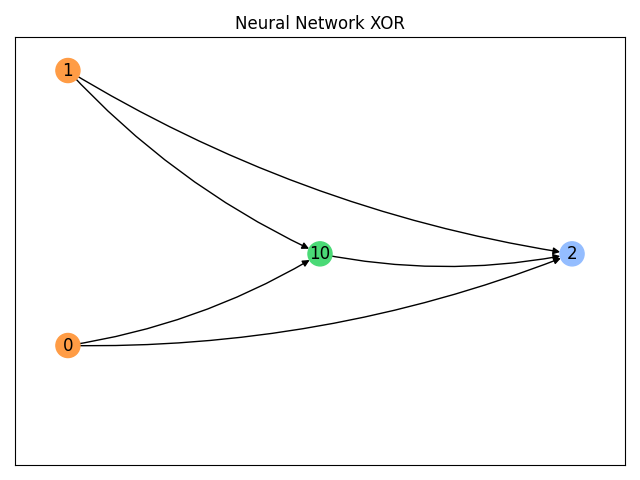
\includegraphics[width=1.0\textwidth]{./img/xor_single_core/xor_neural_network.png} 
		%\caption{Lösung für das XOR-Problem mit einem \emph{Hidden}-Neuron}
		%\label{fig:xor_solution_minimal}
	\end{minipage}
	\hfill
	\begin{minipage}[b]{0.49\textwidth}
		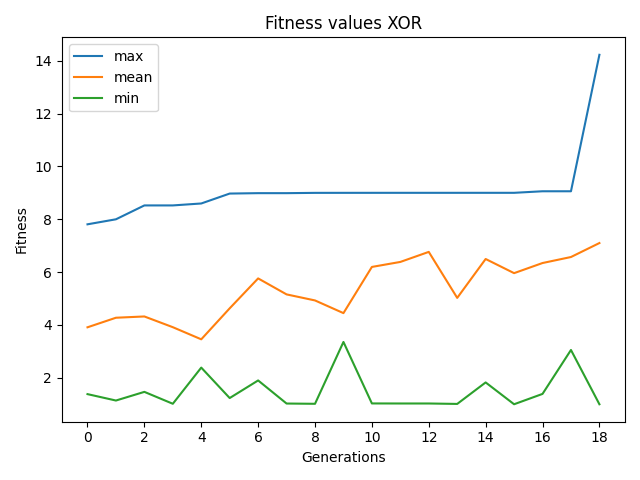
\includegraphics[width=1.0\textwidth]{./img/xor_single_core/xor_fitness_.png} 
		%\caption{Lösung für das XOR-Problem mit einem \emph{Hidden}-Neuron}
	\end{minipage}
	\caption{Links die Lösung für das XOR-Problem mit einem \emph{Hidden}-Neuron, rechts die dazugehörigen Fitnesswerte pro Generation}
	\label{fig:xor_solution_minimal}
\end{figure}
\\\\
Zuletzt soll die tatsächlich erhaltene Lösung genauer betrachtet werden. Im Schnitt hat \ac{NEAT} Lösungen mit 2 oder 3 \emph{Hidden}-Neuronen entwickelt. Allerdings sind auch einige \ac{KNN} entstanden, welche hiervon nur eines und somit die minimale Struktur besitzen, welche zum Lösen des XOR-Problems benötigt wird. Eine solches \ac{KNN}, welches am Ende einer Evaluation entstanden ist, ist in Abbildung \ref{fig:xor_solution_minimal} links dargestellt. Die eigentliche Darstellung ist mithilfe der implementierten Visualisierung  erstellt worden, welche die Pakete NetworkX und Matplotlib nutzt. Bei solchen Darstellungen ist zu beachten, dass die Organgen Neuronen vom Typ \emph{Input}, die grünen vom Typ \emph{Hidden} und die blauen vom Typ \emph{Output} sind. Die Zahlen auf den Neuronen repräsentieren die jeweilige ID während die Pfeile die Verbindungen zwischen den Neuronen darstellen. Für eine bessere Übersichtlichkeit wird in der Darstellung auf die Gewichte verzichtet. Prinzipiell kann eine solche Darstellung auch gestrichelte Verbindungen enthalten. Diese sind dann im Genom deaktiviert und werden nicht für die Berechnungen verwendet. Rechts in der Abbildung ist der Verlauf des maximalen, minimalen und durchschnittlichen Fitnesswertes für jede Generation dargestellt. Auch diese Abbildung wird mit Matplotlib im Rahmen des implementierten \emph{FitnessReporters} automatisch erstellt und zeigt einige interessante Eigenschaften. Der durchschnittliche Fitnesswert steigt trotz einiger Einbrüche relativ kontinuierlich an. Hieraus lässt sich schließen, dass auch die Population im ganzen Fortschritte erzielt. Der maximale Fitnesswert hingegen, stagniert für einige Generationen am Wert $9$. Der Grund hierfür liegt in der Fitnessfunktion. Ein einfaches \ac{KNN} ohne \emph{Hidden}-Neuronen kann drei Werte des XOR-Problems richtig bestimmen. Ist dies der Fall, ergibt die Fitnessfunktion den Wert $9$. Ab diesem Zeitpunkt wird kein Fortschritt des Fitnesswertes erzielt, bis das neue Neuron erfolgreich in die Struktur integriert ist. Der minimale Fitnesswert ist im gesamten Verlauf sehr gering. Der Grund hierfür ist, dass durch unpassende Mutationen oder Rekombinationen Genome entstehen können, bei denen die negativen Eigenschaften überwiegen. 
\begin{figure}[!h]
	\centering
	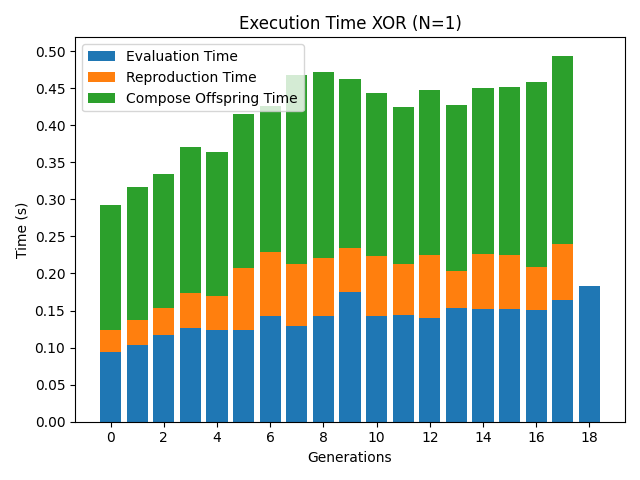
\includegraphics[width=0.5\textwidth]{./img/xor_single_core/xor_time.png} 
	\caption{Ausführungszeiten des XOR-Problems auf einem Raspberry Pi 4 mit einem Prozess}
	\label{fig:xor_single_core_performance}
	% TODO Eventuell Pfeile bei reduce hinzufügen?
\end{figure}
\\\\
Abbildung \ref{fig:xor_single_core_performance} zeigt die Ausführungszeit des Verfahrens in Sekunden für jede Generation an. Auch dieser Graph wird wie die anderen zuvor automatisch mit dem Paket Matplotlib generiert und zeigt drei verschiedene Phasen an. Der blaue Bereich zeigt \emph{Evaluation Time } an, welche die benötigte Evaluationszeit für alle Agenten darstellt. Der grüne Balken repräsentiert die \emph{Compose Offspring Time}, welche die Zeit für die Rekombination und Mutation aller Agenten umfasst. Die verbleibenden Aktionen bezüglich \ac{NEAT}, wie zum Beispiel das Sortieren der Agenten in die verschiedenen Spezies wird im Rahmen der \emph{Reproduction Time} erfasst, welche mit dem grünen Balken repräsentiert wird. Somit wird die Zeit, welche beispielsweise zum Speichern der Zwischenergebnisse benötigt wird nicht erfasst, da diese das Ergebnis verfälschen würde. Insgesamt ist bezüglich des XOR-Problems zu erkennen, dass die Ausführungszeit tendenziell mit zunehmenden Generationen ansteigt. Dies kann durch den erhöhten Rechenaufwand erklärt werden, welcher durch größere \ac{KNN} entsteht. Des weiteren ist auffällig, dass für die letzte Generation keine \emph{Reproduction Time} oder \emph{Compose Offspring Time} erfasst wurde. Der Grund hierfür ist, dass nach der evaluierten Generation die Abbruchbedingung überprüft wird, welche in diesem Fall die Ausführung beendet und daher wird  keine neue Generation erstellt. Zuletzt soll noch die allgemeine Ausführungszeit und das Verhältnis der verschiedenen Phasen betrachtet werden. Zu erkennen ist, dass die Ausführungszeit pro Generation weniger als eine halbe Sekunde benötigt. Dies ist vor allem für Testzwecke ein großer Vorteil, da der Effekt von Änderungen schnell beobachtet werden kann. Zusätzlich ist zu erkennen, dass die meiste Zeit für das Erstellen und Mutieren von neuen Genomen und Agenten benötigt wird. Allerdings ist diese Verteilung unter Umständen nicht repräsentativ, da die XOR-Funktion ein sehr einfaches Problem ist, welches nur wenige Instruktionen umfasst. Daher werden im nächsten Kapitel aufwändigere Optimierungsprobleme betrachtet.

% !TeX spellcheck = de_DE
\section{Optimierungsprobleme}
\label{sec:analysis_optimzation_problems}
Nach erfolgreicher Verifizierung der Funktionalität wird in diesem Kapitel auf verschiedene andere Optimierungsprobleme eingegangen, anhand derer die Analyse durchgeführt werden soll. Grundsätzlich ist bei der Implementierung zu beachten, dass keine zu aufwändigen Optimierungsprobleme verwendet werden, da der Raspberry Pi 4 grundsätzlich nicht so leistungsfähig ist und die benötigte Optimierungszeit sehr hoch sein kann. Daher werden im folgenden hauptsächlich klassische Probleme des bestärkenden Lernens aus dem OpenAI Gym verwendet. Die ausgewählten Umgebungen sind das \emph{Cartpole}, \emph{MountainCar} und das \emph{Pendulum} Problem. Im Folgenden wird auf die entsprechenden Optimierungsprobleme genauer eingegangen und die Implementierung der Fitnessfunktion und Abbruchbedingung kurz vorgestellt. 

\subsection{Cartpole}
Die \emph{Cartpole} Umgebung, auch als \emph{Pole Balancing} bezeichnet, wurde bereits 1983 das erste mal in Quelle \cite{barto1983neuronlike} vorgestellt und ist auch heute noch ein bekanntes Optimierungsproblem, welches in vielen Publikationen verwendet wird. Auch im OpenAI Gym ist dieses Problem entsprechend der Beschreibung aus Quelle \cite{barto1983neuronlike} enthalten und in Abbildung \ref{fig:cartpole_environment} dargestellt. In der Umgebung befinden sich zwei Gegenstände. Das erste ist ein Waagen, welcher von dem Agenten nach links und rechts bewegt werden kann. Hierauf befindet sich ein Balken, welcher am unteren Ende mit dem Waagen verbunden ist. Entsprechend seiner Position, kann dieser nach links oder rechts kippen. Das Ziel für den Agenten ist, durch Steuerung des Wagens den Balken so lange wie möglich senkrecht zu balancieren. Bezüglich der Abbruchbedingung gilt, dass der Agent scheitert wenn der Balken entweder mehr als $15\degree$ auf eine Seite kippt oder wenn der Wagen sich zu weit vom Zentrum entfernt hat. Als Eingabewerte für das \ac{KNN} werden von der Umgebung vier Werte zur Verfügung gestellt, für welche je ein Eingabeneuron erstellt wird. Dies ist unter anderem die Position und Geschwindigkeit des Wagens, der aktuelle Winkel des Balkens und dessen Änderungsrate. Zusätzlich besitzt das erstellte \ac{KNN} zwei Ausgabeneuronen, welche die jeweilige Richtung repräsentieren. Ist der Aktivierungsgrad des erstens \emph{Output}-Neurons höher als der des zweiten, wird der Wagen nach links bewegt und andernfalls nach rechts.
\begin{figure}[!h]
	\centering
	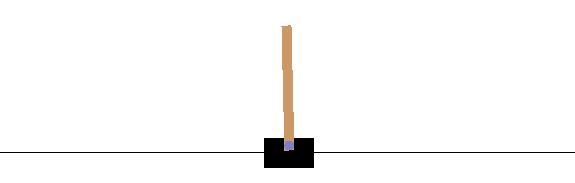
\includegraphics[width=0.5\textwidth]{./img/cartpole_env.JPG} 
	\caption{Darstellung der \emph{Cartpole} Umgebung}
	\label{fig:cartpole_environment}
\end{figure} 
Bevor die Evaluation mit dieser Umgebung durchgeführt wird, müssen noch die Fitnessfunktion, Lösungsbedingung und Konfiguration festgelegt werden. Beim klassischen bestärkenden Lernen, wie es in Kapitel \ref{subsubsec:reinforcment_learning} beschrieben ist, erhält der Agent nach jedem Zeitschritt einen \emph{reward}. Da das OpenAI Gym primär für diese Art des Lernens konzipiert ist, wird auch hier nach jeder Aktion in der Umgebung ein \emph{reward} zurück gegeben. In diesem Fall erhält ein Agent bis er scheitert für jeden Zeitschritt einen \emph{reward} mit der Wertigkeit $1$. Mit diesen muss für neuroevolutionäre Algorithmen eine Fitnessfunktion definiert werden. In diesem Beispiel ist das Vorgehen einfach. Der Fitnesswert wird berechnet indem die erhaltenen \emph{rewards} aggregiert und der erhaltene Wert am Ende der Evaluation quadriert wird. Somit soll wie zuvor beim XOR-Problem besseren Agenten ein proportional höherer Fitnesswert zugewiesen werden. Das Optimierungsverfahren wird abgebrochen, wenn ein Agent den Balken für mindestens 500 Zeitschritte balancieren kann. Die restlichen Parameter wurden aus dem vorherigen Beispiel übernommen und nicht wieder geändert.
\begin{figure}[!h]
	\centering
	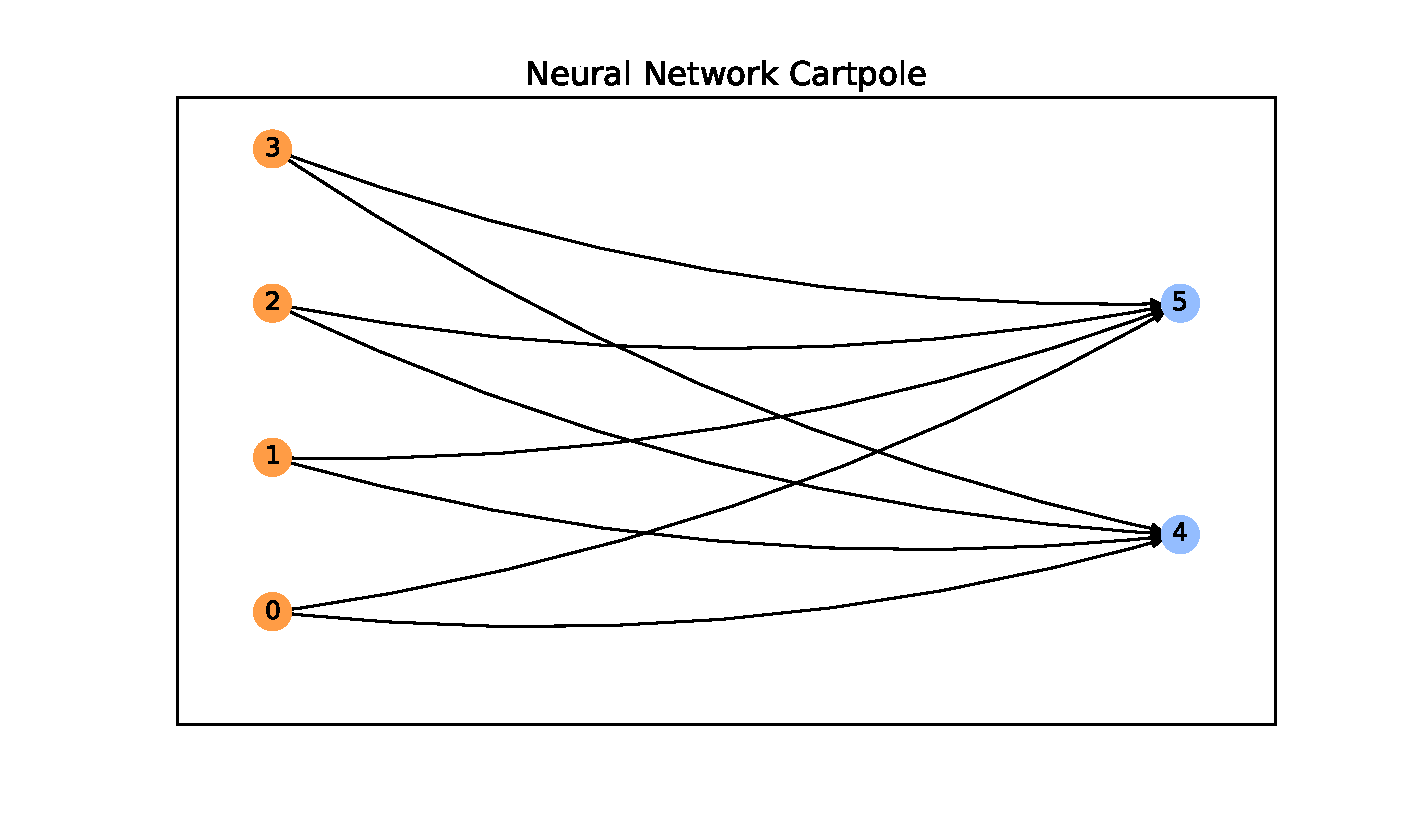
\includegraphics[width=0.7\textwidth]{./img/pole_balancing_single_core/cartpole_neuroal_network.pdf} 
	\caption{Struktur des finalen \ac{KNN} im \emph{Cartpole} Optimierungsproblem}
	\label{fig:cartpole_neural_network}
\end{figure}
\\\\
Allerdings stellt sich beim Ausführen dieses Optimierungsproblems heraus, dass es für die Analyse ungeeignet ist. Bereits in der initialen Population, für welche die Agenten zufällig erstellt werden, sind \ac{KNN} vorhanden, die die Abbruchbedingung erfüllen und das Optimierungsproblem lösen. Ein solches ist in Abbildung \ref{fig:cartpole_neural_network} dargestellt. Wie die anderen \ac{KNN} in der initialen Population, besitzt auch dieses keine \emph{Hidden}-Neuronen und zeigt, dass für das Lösen dieses Optimierungsproblem keine komplexen Entscheidungen notwendig sind. Es ist beispielsweise mit dem Winkel des Balken möglich auf die auszuführende Aktion zu schließen. Neigt sich der Balken nach rechts, bewegt sich der Wagen in diese Richtung und umgekehrt. Dies ist einer der Gründe warum dieses Optimierungsproblem im weiteren Verlauf der Arbeit nicht weiter verwendet wird. Ein weiterer Grund ist, dass durch die Fehlende Optimierung keine Ausführungszeiten über mehrere Generationen gemessen werden können, welche eine notwendige Grundlage für den späteren Vergleich sind.

\subsection{Mountain Car}

\subsection{Pendulum}



% !TeX spellcheck = de_DE
\section{Erkenntnisse}
\label{sec:analysis_results}
Nach Darstellung der Optimierungsprobleme erfolgt eine Zusammenfassung der Ergebnisse in diesem Kapitel. Alle vorgestellten Optimierungsverfahren konnten durch die Schnittstelle der Bibliothek schnell und einfach implementiert werden. Dies trifft sowohl auf individuell erstellte Optimierungsprobleme als auch auf Standardprobleme aus dem \emph{OpenAI Gym} zu. Auch die restlichen Anforderungen aus Kapitel \ref{sec:requirements} sind vollständig implementiert. Der gesamte Ablauf des Algorithmus kann mithilfe eines spezifizierten \emph{Seeds} beeinflusst und wiederholt werden. Die verschiedenen Abbildungen im vorherigen Kapitel zeigen, dass die Testergebnisse der Trainingsverfahren gemessen, visualisiert und gespeichert werden können, sodass ein späterer Vergleich mit der parallelisierten Implementierung möglich ist.
\\\\
Die Funktionalität des Algorithmus, neue Strukturen zu entwickeln und zu optimieren, ist mit dem XOR-Problem bewiesen. Mit derselben Konfiguration werden im Vergleich zur originalen Implementierung ähnliche Ergebnisse gemessen. Durch verschiedene Anpassungen konnten bei nachfolgenden Versuchen sogar bedeutend bessere Ergebnisse erzielt werden. Bei Betrachtung der Ausführungszeit ist in diesem Beispiel die Zeit zum Erstellen und Mutieren von Nachkommen der größte Faktor. Aber da das XOR-Problem insgesamt sehr einfach ist und somit aufwendigere Probleme nicht richtig repräsentiert, finden die Ergebnisse im weiteren Verlauf keine Beachtung.
\\\\
Im nächsten Schritt wurden daher die \emph{CartPole}, \emph{MountainCar} und \emph{Pendulum} Umgebung des \emph{OpenAI Gyms} implementiert, welche aufwendiger zu lösen sein sollten als das XOR-Problem. Die Tests haben ergeben, dass die erste Umgebung ungeeignet ist, da bereits die zufällig erstellten \ac{KNN} der ersten Generation das Optimierungsproblem lösen können. Dies trifft nicht auf die zwei anderen Umgebungen zu. Im vorgestellten Szenario wurden für die erste Umgebung $105$ Minuten, für die zweite Umgebung $125$ Minuten zur erfolgreichen Optimierung benötigt. Zwar hat \ac{NEAT} beide Probleme erfolgreich gelöst, dennoch werden die Grenzen des Algorithmus aufgezeigt. Vor allem auf dem Raspberry Pi sind die benötigten Optimierungszeiten für verhältnismäßig kleine Probleme sehr hoch. Große Optimierungsprobleme, bei denen die Eingabevektoren aus mehreren tausend Werten bestehen, können aufgrund der begrenzten Rechenleistung nicht oder nur mit sehr hohem Zeitaufwand optimiert werden. Da der Fokus dieser Arbeit auf dem Vergleich zwischen einer sequenziellen und parallelisierten Implementierung liegt, ist dieser Umstand zu vernachlässigen.
\\\\
Bei Betrachtung der Ausführungszeiten ist sowohl für das \emph{MountainCar} und \emph{Pendulum} Problem ersichtlich, dass die Evaluationsphase der größte Faktor ist. In der ersten Umgebung werden $98\%$, in der zweiten $91\%$ der Ausführungszeit für das Erstellen und Evaluieren der \ac{KNN} verwendet. Da im Falle einer erfolgreichen Parallelisierung in dieser Phase die meiste Ausführungszeit eingespart werden kann, liegt der Fokus im folgenden Kapitel primär darauf. Für die eigentliche Parallelisierung ist wichtig, dass nicht nur die Berechnungen des \ac{KNN} optimiert werden. Im Rahmen der \emph{Evaluation Time} wird neben der benötigten Zeit zum Erstellen und Aktivieren eines \ac{KNN} auch die benötigte Zeit zum Simulieren der Umgebung gemessen. Diese kann einen großen Einfluss auf das Gesamtergebnis haben. An zweiter und dritter Stelle der Priorisierung stehen die Parallelisierungen der Funktionen in den Phasen \emph{Compose Offspring Time} und \emph{Reproduction Time}. Beide haben einen bedeutend geringeren Anteil an der gesamten Ausführungszeit und dementsprechend weniger Zeit kann eingespart werden. Ob und wie diese implementiert werden können, wird in den Kapiteln \ref{sec:future_work} erläutert.
\\\\
Zuletzt soll betont werden, dass bei den vorgestellten Optimierungsproblemen keine generelle Lösungsstrategie entwickelt wird. Hierfür müssten verschiedene Startsituationen in der Evaluationsphase getestet werden, indem beispielsweise jeder Agent in $x$ verschiedenen Umgebungen getestet und der mittlere Fitnesswert verwendet wird. Dies würde die Evaluationszeit um den Faktor $x$ erhöhen, was im gegebenen Anwendungsszenario eine Analyse bedeutend aufwendiger gestalten würde. Mit der parallelisierten Version in Kapitel \ref{sec:lunar_lander} kann ein solches Verfahren umgesetzt und ein entsprechendes \ac{KNN} schneller entwickelt werden.



% !TeX spellcheck = de_DE
\chapter{Optimierung}

% Mehrere Arten der Optimierung, in diesem Fall soll die Parallelisierung eingesetzt werden

% Optimierung am anfang schlecht, Eventuell probleme mit kurzer trainingszeit, deswegen erhöhen auf 10 pro run, trotzdem schlecht, danach testen mit verschiedenen devices

% Wenig abweichung von ideal wert, zeigt gute parallelisierung

% !TeX spellcheck = de_DE
\section{Strategien zur Parallelisierung}
\label{sec:parallel_strategies}
Es gibt mehrere Möglichkeiten zur Umsetzung einer Parallelisierung sowie verschiedene Schwerpunkte, welche diese haben kann. Die Analyse der sequenziellen Implementierung hat gezeigt, dass die \emph{Evaluation Time} den größten Einfluss auf die Ausführungszeit hat.  Dementsprechend kann bei einer erfolgreichen Parallelisierung dieser Phase die größte Reduktion der Ausführungszeit erzielt werden. Aus diesem Grund liegt der Fokus im Weiteren hierauf. 
\begin{figure}[!h]
	\centering
	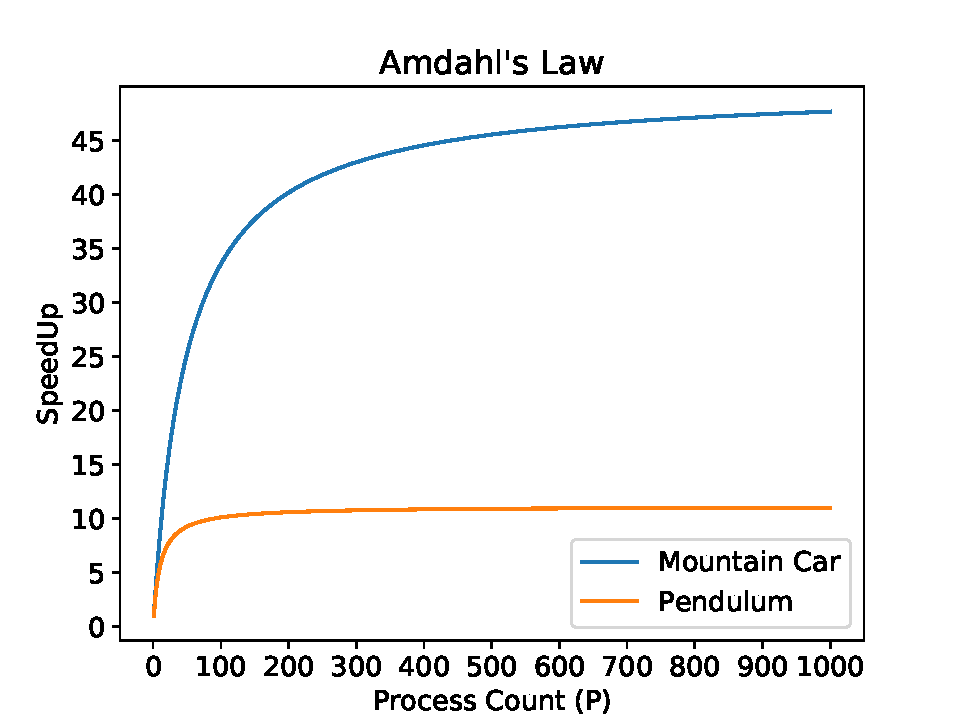
\includegraphics[width=0.5\textwidth]{./img/ahmdals_law_mountain_pendulum.pdf} 
	\caption{Durch \emph{Amdahl's Law} berechnete theoretische \emph{SpeedUp} für das \emph{Mountain Car} und \emph{Pendulum} Problem in Abhängigkeit der Anzahl an Prozessen}
	\label{fig:amdahls_law_mountain_pendulum}
\end{figure}
Mit \emph{Amdahl's Law}, welches in Kapitel \ref{subsec:basics_performance} vorgestellt ist, kann der theoretisch erreichbare \emph{SpeedUp} in Abhängigkeit von $P$ Prozessoren berechnet werden. Dies ist in Abbildung \ref{fig:amdahls_law_mountain_pendulum} dargestellt, wobei entsprechend der Analyseergebnisse angenommen wird, dass die \emph{Mountain Car} Umgebung zu $98\%$ und die \emph{Pendulum} Umgebung zu $91\%$ parallelisiert werden können. Durch die Abbildung ist ersichtlich, dass beide Probleme anfänglich mit steigender Anzahl an Prozessen sehr gute \emph{SpeedUp} Werte erzielen. Allerdings ist das Hinzufügen von weiterer Rechenleistung ab einem gewissen Punkt nicht mehr effektiv, da der Anstieg des \emph{SpeedUps} zunehmend geringer wird und schlussendlich gegen einen gewissen Wert konvergiert. Für $P \rightarrow \infty$ liegt der maximale \emph{SpeedUp} für die \emph{Mountain Car} Umgebung bei Faktor 50 und für die \emph{Pendulum} Umgebung bei Faktor $11.\overline{1}$. Auch wenn diese Ergebnisse eine ungefähre Richtlinie bieten, ist das Erreichen dieser Vorgaben in einer praktischen Umsetzung unwahrscheinlich. Durch eine hohe Anzahl an beteiligten Prozessen entsteht in der Regel ein hoher Kommunikationsaufwand, der sich negativ auf den \emph{SpeedUp} Wert auswirkt. Im Folgenden werden verschiedene Strategien zur Umsetzung einer möglichst effizienten Parallelisierung aufgezeigt und die verschiedenen Vor- und Nachteile gegeneinander abgewogen.
\\\\
Vor dem Auswählen einer geeigneten Strategie sollen die zu parallelisierenden Funktionen der \emph{Evaluation Time} analysiert werden. Im sequenziellen Verfahren wird in dieser Phase über eine Liste mit allen Agenten iteriert. Für jeden von diesen wird die Umgebung einmal zurückgesetzt und ein \ac{KNN} aus dem Genom des Agenten gebildet. Danach wird die Umgebung simuliert. Bei diesem Vorgang können beliebig viele Simulationsschritte und Aktivierungen des \ac{KNN} ausgeführt werden. 
\\\\
Ein möglicher Ansatz besteht darin, die Berechnungen in einem \ac{KNN} selbst zu parallelisieren. Dies ist eine valide Strategie, die unter anderem von Bibliotheken wie \emph{Tensorflow} und \emph{PyTorch} genutzt wird. Die einzelnen Neuronen einer Schicht können beispielsweise unabhängig voneinander aktiviert und somit auch parallelisiert werden. Zusätzlich kann eine solche Parallelisierung nicht nur mithilfe von \acp{CPU}, sondern auch auf \acp{GPU} umgesetzt werden. Diese haben in der Regel mehr unabhängige Prozessoren als normale \acp{CPU}, wodurch in vielen Fällen eine bessere Parallelisierung ermöglicht wird. Allerdings sprechen zwei Gründe gegen den Einsatz einer solchen Parallelisierungsstrategie in dieser Arbeit. Die vorgestellten Bibliotheken implementieren diese Funktionalitäten bereits, sind weit verbreitet und für verschiedene Plattformen optimiert. Zusätzlich ist es im Rahmen einer zukünftigen Erweiterung möglich, diese einfach in dieses Projekt zu integrieren. Daher ist es nicht sinnvoll, Ressourcen für die Implementierung derselben Funktionalität zu verwenden. Der zweite Grund, der gegen diese Art der Parallelisierung spricht, besteht darin, dass zwar die Aktivierungszeit des \ac{KNN}, jedoch nicht die Simulationszeit der Umgebung verkürzt wird. Diese kann je nach Komplexität des Problems sehr viel Rechenzeit in Anspruch nehmen. 
\\\\
Hier können neuroevolutionäre Algorithmen einen Vorteil bieten, da sowohl das \ac{KNN} als auch die Umgebung parallelisierbar sind. Die Idee ist, dass jeder beteiligte Prozess eine Kopie des Optimierungsproblems initialisiert. Während des Verfahrens wird jeder Agent einem Prozess zugewiesen. Dieser kann unabhängig von anderen Prozessen ein \ac{KNN} aus dem Genom erzeugen und mit diesem die gesamte Evaluation in der lokalen Umgebung durchführen. Am Ende wird nur der Fitnesswert als Ergebnis übertragen. Dieses Vorgehen bietet mehrere Vorteile. Mit dieser Strategie werden alle Funktionen der \emph{Evaluation Time} parallelisiert, inklusive des Optimierungsproblems und der Berechnungen im \ac{KNN}. In einer späteren Erweiterung kann zusätzlich eine Bibliothek wie \emph{Tensorflow} integriert werden, welche die benötigte Zeit zum Berechnen des \ac{KNN} reduziert und somit einen noch größeren \emph{SpeedUp} ermöglicht. Ein weiterer Vorteil ist die geringe Anzahl an benötigten Nachrichten. Mit $n$ Agenten müssen theoretisch nur $2 \cdot n$ Nachrichten pro Generation für die Parallelisierung der \emph{Evaluation Time} ausgetauscht werden. Hiervon wird eine Hälfte zum Verteilen der Agenten und die andere Hälfte zum Sammeln der berechneten Fitnesswerte am Ende der Evaluation benötigt. Durch diese effiziente Kommunikation ist der zusätzlich entstehende Rechenaufwand sehr gering und das Erreichen einer effizienten Parallelisierung möglich.

 



% Client Server can prevent deadlocks
% Eventually calculate ahmdals law?
% !TeX spellcheck = de_DE
\section{Implementierung}
\label{sec:parallel_implementation}
Dieses Kapitel befasst sich mit der Implementierung der bereits vorgestellten Parallelisierungsstrategie. Das Ziel ist, die Ausführungszeit des Verfahrens in einem verteilten System durch Hinzufügen von weiteren Prozessoren zu reduzieren. Bei der Umsetzung sind drei Anforderungen zu beachten. Erstens muss es mit geringem Aufwand möglich sein, die sequenzielle Implementierung durch die parallelisierte auszutauschen und umgekehrt. Zweitens muss für eine Bewertung der Effizienz der Parallelisierung ein direkter Vergleich zwischen beiden Implementierungen möglich sein. Drittens ist der Standard \ac{MPI} für die Kommunikation zu verwenden
\\\\
Für die parallelisierte Implementierung wird eine neue Klasse angelegt, die von dem in Kapitel \ref{subsubsec:library_interface} vorgestellten Interface \emph{NeatOptimizer} erbt. Da auch die sequenzielle Implementierung dieses verwendet, ist die erste Anforderung bereits erfüllt. Beide Klassen stellen dieselben Funktionen zur Verfügung und können somit jederzeit gegeneinander ausgetauscht werden. Wie in Kapitel \ref{subsubsec:library_interface} erläutert, ist die \emph{evaluate()} Funktion in diesem Interface der Einstiegspunkt für die Bibliothek und das gesamte Trainingsverfahren ist in dieser implementiert. 
\\\\
Um die zweite Anforderung zu erfüllen, ist der grundsätzliche Ablauf der \emph{evaluate()} Funktion identisch zum sequenziellen Verfahren, sodass sich nur der parallelisierte Teil des Programms unterscheidet. Zu Beginn des Trainingsverfahrens wird eine initiale Population generiert. Danach beginnt eine Schleife, in welcher die Funktionen \emph{build\_new\_generation()} und \emph{evaluate\_generation()} abwechselnd aufgerufen werden bis die Abbruchbedingung erfüllt ist. Da primär die Evaluationsphase parallelisiert wird, kann die \emph{build\_new\_generation()} Funktion vom sequenziellen Verfahren unverändert übernommen werden. In dieser sind die Phasen Selektion, Rekombination und Mutation implementiert. Die Funktion \emph{evaluate\_generation()} umfasst die Evaluation der Agenten. Da die Analyse zeigt, dass sowohl in der \emph{Mountain Car} als auch in der \emph{Pendulum} Umgebung diese Funktion den größten Einfluss auf die benötigte Rechenzeit hat, wird sie im Rahmen der Parallelisierung neu implementiert.
\\\\
Im sequenziellen Verfahren wird bei der Evaluationsphase über die Liste mit allen Agenten iteriert und für jeden nacheinander die Evaluation durchgeführt. Wie bereits in Kapitel \ref{sec:sequential_implementation} beschrieben, wird hierfür vor jedem neuen Agenten die Umgebung einmalig zurückgesetzt, das \ac{KNN} gebildet und die eigentliche Evaluation mit dem Ziel durchgeführt, am Ende einen Fitnesswert zurückzugeben. Bei der parallelisierten Implementierung werden die Agenten an alle beteiligten Prozesse verteilt, welche dann die Evaluation unabhängig voneinander durchführen. 
\\\\
Dafür muss im nächsten Schritt die Art der Kommunikation und Verteilung der Agenten festgelegt werden. In Kapitel \ref{subsec:mpi} sind die \emph{Scatter} und \emph{Gather} Funktion vorgestellt, welche sich prinzipiell für dieses Szenario anbieten. Die \emph{Scatter} Funktion verteilt die Agenten gleichmäßig auf die Prozesse und die \emph{Gather} Funktion sammelt die Ergebnisse. Zwar ist die Implementierung effizient, es ergibt sich aber ein gewichtiger Nachteil. Die \emph{Scatter} Funktion erlaubt keine dynamische Verteilungen von Lasten, was in diesem Projekt jedoch aus zwei Gründen sinnvoll ist. Der erste Grund betrifft die Evaluationszeiten, der zweite die Struktur des Clusters. Die Evaluationszeiten der Agenten unterscheiden sich in vielen Fällen. Gründe hierfür können zum einen unterschiedlich große \ac{KNN} sein, deren Berechnungszeit bzw. Aktivierungszeit variiert, zum anderen unterschiedliche Fortschritte im Optimierungsproblem. In der vorgestellten \emph{Mountain Car} Umgebung wird beispielsweise die Evaluation beendet, wenn der Agent das Ziel erreicht. In anderen Optimierungsproblemen kann die Evaluation frühzeitig abgebrochen werden, wenn ein Agent eine bestimmte Fehlentscheidung getroffen hat. Die Folge in beiden Szenarien ist, dass im Vergleich zu anderen Prozessen weniger Rechenaufwand für die Evaluation des Agenten benötigt wird. Hierdurch entsteht ein Ungleichgewicht in der Lastenverteilung. Die Folge ist, dass am Ende einer Evaluationsphase die Prozesse aufeinander warten. Somit sinkt die Effizienz und auch der erreichte \emph{SpeedUp} Wert der Parallelisierung. Auch wenn alle Agenten dieselbe Rechenlast erzeugen und diese gleichmäßig auf alle Prozesse verteilt ist, kann es in einem Beowulf Cluster zu Wartezeiten kommen. Grund hierfür ist, dass sich die Konfiguration der Hardware bei den einzelnen Geräten des Clusters und somit auch deren Leistung unterscheiden kann. Für eine gute Performance des parallelisierten Verfahrens müssen die Prozessoren bzw. Geräte des Clusters, welche mehr Rechenleistung bieten, auch proportional mehr Rechenlast zugewiesen bekommen. Dies ist mit der \emph{Scatter} Funktion nicht möglich.
\\\\
Daher soll in dieser Arbeit die \emph{Point-to-Point} Kommunikation verwendet werden, mit welcher ein dynamisches Zuteilen möglich ist. Um mögliche \emph{Deadlocks} zu vermeiden, wird eine \emph{Master-Slave} Architektur gewählt. Zu Beginn der Evaluationsphase erstellt der \emph{Master} Prozess verschiedene Arbeitspakete, welche jeweils einen zu evaluierenden Agenten enthalten. Initial wird an jeden \emph{Slave} Prozess asynchron ein Paket gesendet, welche hierauf warten. Ist dieses vollständig empfangen, wird der darin enthaltene Agent im lokalen Optimierungsproblem evaluiert und der berechnete Fitnesswert als Ergebnis an den \emph{Master} Prozess zurückgesendet. Dieser ist für die Speicherung zuständig. Danach wird überprüft, ob noch weitere Arbeitspakete zur Abarbeitung ausstehen. Ist dies der Fall, wird ein neues Pakt an den \emph{Slave} übermittelt. Erst wenn alle Pakete abgearbeitet sind, endet die Evaluation der Generation. Danach führt der \emph{Master} Prozess die erforderlichen Operationen zum Erzeugen der nächsten Generation aus. Dabei werden die gespeicherten Ergebnisse der \emph{Slaves} verwendet. Mit der neuen Generation beginnt die Evaluation erneut. Ein großer Vorteil dieses Verfahrens ist, dass Prozesse automatisch mehr Arbeitspakete zugeteilt bekommen, wenn sie entweder leistungsfähiger oder die Evaluationszeiten der Agenten kürzer sind. Zusätzlich ist die Kommunikationsstruktur strikt geregelt, sodass das Auftreten von \emph{Deadlocks} unwahrscheinlich ist.
\\\\
Für die praktische Umsetzung muss der Implementierung noch die Klasse \emph{Slave} hinzugefügt werden, welche die notwendigen Operationen enthält. Dies umfasst die Funktion \emph{setup()}, welche zum Erstellen des Optimierungsproblems bzw. der Umgebung benötigt wird und die Funktion \emph{evaluate\_agent()}. Als Parameter wird dieser Funktion ein Agent übergeben, der dann evaluiert wird. Im Rahmen dessen wird die Umgebung auf den Startzustand gesetzt, ein \ac{KNN} mit dem Genom des Agenten erzeugt und die eigentliche Evaluation in der lokalen Umgebung durchgeführt. Die Funktion gibt am Ende den Fitnesswert sowie optionale Zusatzinformationen der Umgebung zurück. Insgesamt entspricht diese Funktionalität der des sequenziellen Verfahrens. Die \emph{setup()} Funktion erstellt die Umgebung, benötigt aber einen anderen Implementierungsansatz als die \emph{evaluate\_agent()} Funktion. Der Grund hierfür ist der Parameter. Ein Agent enthält nur Daten, aber keine Funktionalität. Aus diesem Grund kann er einfach mit \ac{MPI} serialisiert und versendet werden. Ein Optimierungsproblem hingegen kann eine komplexe Klasse mit unterschiedlichen Funktionen sein, die unter Umständen nicht serialisiert werden können. Zusätzlich sind in der implementierte Bibliothek keine Informationen über die Funktionalitäten, Architektur und den internen Zustand der Umgebung enthalten. Grund hierfür ist, dass neue Optimierungsprobleme von Nutzern jederzeit hinzugefügt werden können und es diesbezüglich keine Einschränkungen geben soll. Daher kann das Optimierungsproblem nicht mit \ac{MPI} serialisiert werden. Stattdessen wird der Umstand genutzt, dass der Programmcode auf jedem beteiligten Gerät bzw. Prozessor vorliegen muss. Beim Starten einer \ac{MPI} Anwendung wird auf jedem beteiligten Prozess eine Kopie des Programms ausgeführt. Hierbei kann jeder Prozess auf Basis des zugewiesenen Rangs entscheiden, ob er die Funktion eines \emph{Masters} oder \emph{Slaves} einnimmt. Der \emph{Master} führt die notwendigen Operationen zum Erstellen der initialen Generation durch und startet den Optimierungsprozess. Die \emph{Slaves} greifen auf das im Programmcode vorliegende Optimierungsproblem zu und initialisieren es. Bei einem solchen Vorgehen ist es nicht erforderlich, das Optimierungsproblem zu serialisieren und zu versenden.
\\\\
Der letzte hier vorgestellte Implementierungsaspekt bezieht sich auf die Umsetzung der \emph{Point-to-Point} Kommunikation. Hierfür wird das Paket \emph{mpi4py} verwendet, welches eine Python Schnittstelle zum Nutzen von \ac{MPI} Funktionen bietet. Das Paket selbst ist \emph{open source} verfügbar und im Vergleich zu anderen Implementierungen weit verbreitet. Zusätzlich bietet es eine gute Performance, welche in Quelle \cite{dalcin2008mpi} gemessen wurde, und ist nur geringfügig langsamer als eine Implementierung in der Programmiersprache C. Ein letzter entscheidender Vorteil sind verschiedene in der Bibliothek implementierte high-level Funktionen. Diese ermöglichen unter anderem das einfache Umsetzen der oben beschriebenen \emph{Master-Slave} Kommunikation. Diese Funktionen werden in dieser Arbeit für die Kommunikation verwendet.

% !TeX spellcheck = de_DE
\section{Testumgebung} % TODO ABBILDUNG
\label{sec:test_env_parallel}
Das nächste Kapitel befasst sich mit der Evaluation des parallelisierten Verfahrens und führt einen Vergleich mit der sequenziellen Implementierung durch. Zuvor wird in diesem Kapitel auf die verwendete Testumgebung sowie die Installation der notwendigen Software eingegangen. 
\\\\
Der größte Unterschied dieser Testumgebung im Vergleich zu der des sequenziellen Verfahrens besteht darin, dass das parallelisierte Verfahren nicht auf einem Raspberry Pi 4, sondern auf einem Beowulf-Cluster ausgeführt wird, welcher schematisch in Abbildung (TODO ABBILDUNG) dargestellt ist. Insgesamt stehen zehn identisch konfigurierte Raspberry Pi 4 \emph{Nodes} zur Verfügung. Die Hardware von diesen entspricht der Beschreibung in Kapitel \ref{sec:analysis_testsetup}. Somit besitzt der entstehende Cluster die zehnfache Rechenleistung im Vergleich zu der Testumgebung des sequenziellen Verfahrens.
\\\\
Entsprechend  der in Kapitel \ref{subsubsec:beowulf_cluster} definierten Anforderungen an einen Beowulf Cluster ist jeder Raspberry Pi durch eine Ethernet Verbindung mit einem Netzwerkswitch verbunden. Die maximale Bandbreite für jeden Raspberry Pi beträgt ein Gigabit. Hinsichtlich der Software wird das bisher verwendete Betriebssystem sowie alle Softwarepakete von der sequenziellen Testumgebung übernommen. Allerdings werden für die Kommunikation im Beowulf Cluster noch weitere Softwarekomponenten benötigt. Zuerst wird das MPICH installiert. Wie in Kapitel \ref{subsec:mpi} beschrieben, ist dies eine weit verbreitete \emph{open source} Implementierung des \ac{MPI} Standards. Zusätzlich wird in der Python Umgebung das bereits vorgestellte Paket \emph{mpi4py} installiert, welches den Zugriff auf \ac{MPI} Funktionen aus Python ermöglicht. Ab diesem Zeitpunkt kann die Implementierung lokal getestet werden. Dennoch kann das Verfahren noch nicht auf dem gesamten Beowulf Cluster ausgeführt werden, da die einzelnen \emph{Nodes} noch nicht miteinander kommunizieren können. Hierfür wird zusätzlich das \ac{SSH} Protokoll benötigt. Beim Beginn der Ausführung eines \ac{MPI} Programms wird eine \ac{SSH} Verbindung von jedem teilnehmenden Prozess zu allen anderen erstellt, über welche dann die spätere \ac{MPI} Kommunikation erfolgt. Für die Authentifizierung im \ac{SSH} Protokoll wird in diesem Fall ein asymmetrischer kryptographischer Schlüssel benötigt. Auf jedem Raspberry Pi wird hiervon einer erzeugt, welcher aus einem öffentlichen und privaten Teil besteht. Von jedem Raspberry Pi wird der öffentliche Teil des Schlüssels auf den anderen Geräten des Clusters hinterlegt, sodass eine Authentifizierung ohne Passworteingabe möglich ist.
\\\\
Nach Konfiguration des \ac{SSH} Protokolls kann das Optimierungsverfahren gestartet werden, sobald der Programmcode auf allen beteiligten Geräten vorliegt. Prinzipiell kann dieser manuell an jede einzelne \emph{Node} verteilt werden. Dies ist zeitaufwendig und nicht für die aktive Entwicklung geeignet, daher wird in dieser Testumgebung eine automatisierte Lösung angestrebt. Wie in Kapitel \ref{subsubsec:beowulf_cluster} beschrieben, kann die \emph{Master Node} eines Beowulf Clusters verschiedene organisatorische Aufgaben übernehmen. In diesem Projekt gehört hierzu unter anderem eine Schnittstelle zu den externen Umgebungen, über welche das Optimierungsverfahren gestartet werden kann. Zusätzlich wird für die automatisierte Verteilung des Programmcodes ein Ordner im Netzwerk des Beowulf Clusters freigegeben. Dieser kann von den \emph{Slaves} lokal hinzufügt werden. Der Programmcode bzw. die benötigten Dateien müssen auf dem \emph{Master} im freigegebenen Ordner vorhanden sein. Mit entsprechender Standardsoftware kann eine automatisierte Verteilung und Synchronisation der Dateien umgesetzt werden. Änderungen sind direkt auf allen \emph{Slaves} verfügbar und fehlende oder inkonsistente Dateien werden vermieden.

% !TeX spellcheck = de_DE
\section{Evaluation}
Nachdem die Parallelisierung der Evaluationsphase durchgeführt und die Testumgebung spezifiziert ist, wird in diesem Kapitel die Performance des Verfahrens gemessen. Die hierbei erhaltenen Ergebnisse werden mit denen der sequenziellen Implementierung verglichen. Im letzten Schritt wird eine Bewertung bezüglich der Effizienz und des \emph{SpeedUps} abgegeben.

\subsection{Mountain Car}
\label{subsec:mountain_car_optimzation}
Das parallelisierte Verfahren wird zuerst in der \emph{Mountain Car} Umgebung getestet, die aus Kapitel \ref{subsec:analysis_mountain_car} bekannt ist. Mit dem Ziel, einen einfachen Vergleich zwischen der sequenziellen und parallelisierten Implementierung zu ermöglichen, wird die zuvor verwendete Konfiguration des Verfahrens vollständig übernommen. Selbiges gilt für den \emph{Seed}. Bei korrekter Implementierung des parallelisierten Verfahrens werden dieselben Zwischenergebnisse nach jeder Generation generiert und das finale Ergebnis stimmt mit dem des sequenziellen Verfahrens überein. Somit kann keine Implementierung einen zeitlichen Vorteil erlagen, der durch bessere Agenten oder kürzere Evaluationszeiten entsteht. Beide Implementierungen werden dieselben Berechnungen und Evaluationen durchführen.
\begin{figure}[!h]
	\centering
	\begin{minipage}[]{0.49\textwidth}
		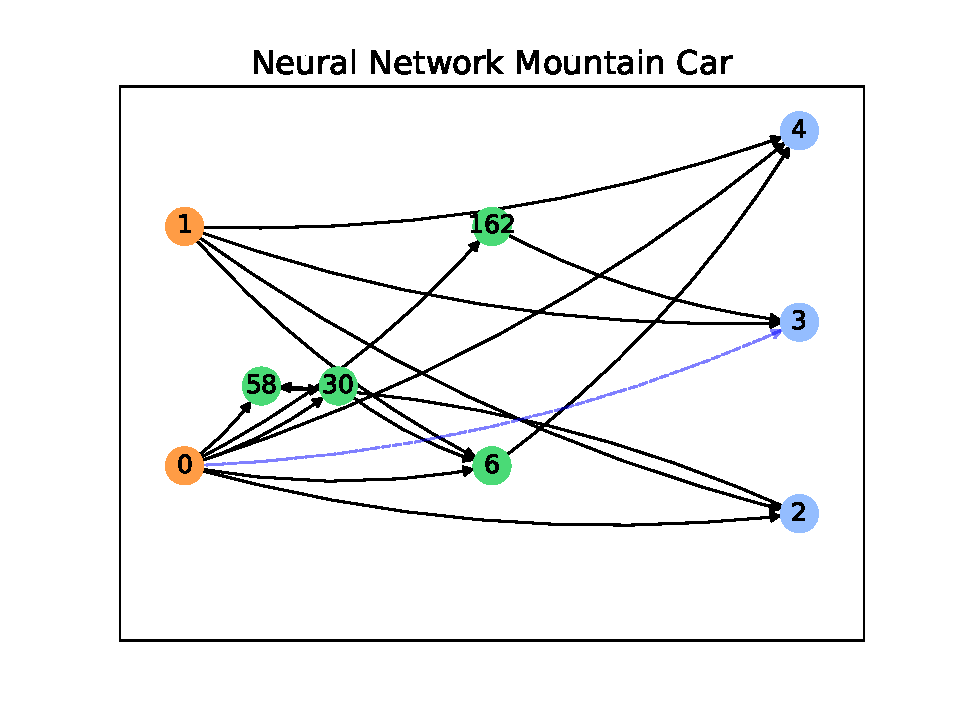
\includegraphics[width=1.0\textwidth]{./img/mountain_car_single/mountain_car_neural_network.pdf} 
	\end{minipage}
	\hfill
	\begin{minipage}[]{0.49\textwidth}
		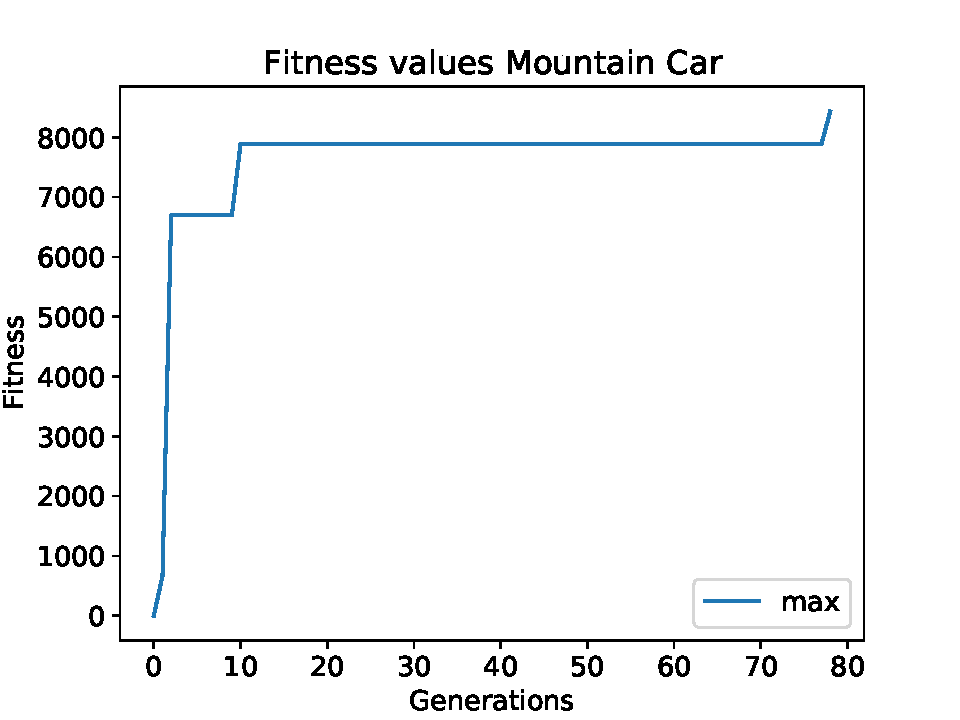
\includegraphics[width=1.0\textwidth]{./img/mountain_car_single/1413_fitness_1core_1pi.pdf} 
	\end{minipage}
	\caption{Links die Lösung für das Mountain Car Problem, rechts die dazugehörigen Fitnesswerte pro Generation mit 10 Prozessen}
	\label{fig:mountain_car_10core_neural_network_and_fitness}
\end{figure}
\begin{figure}[!h]
	\centering
	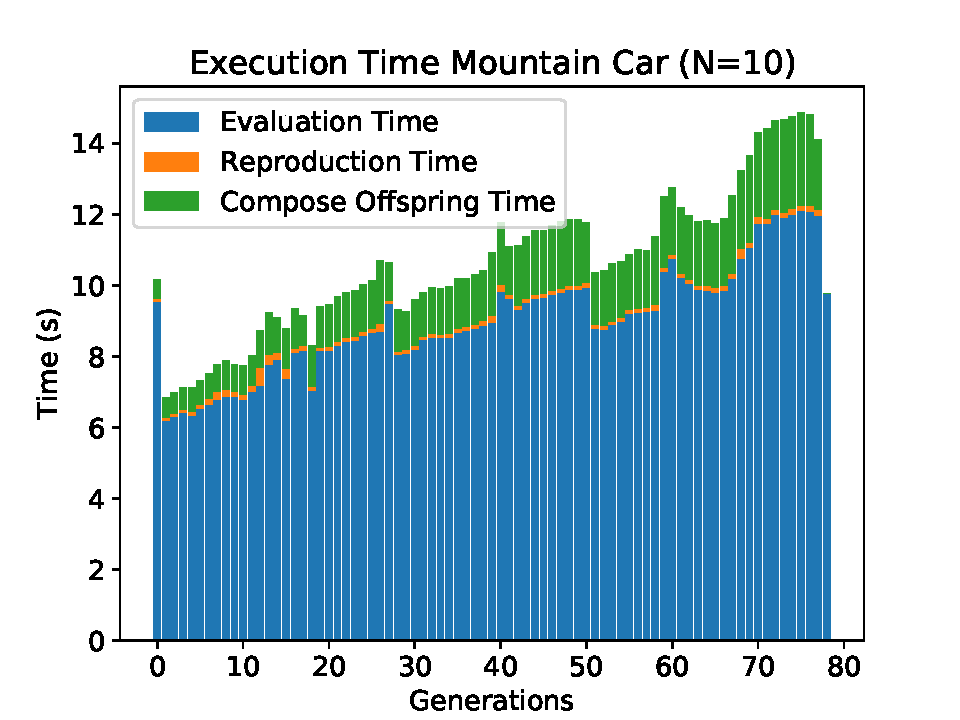
\includegraphics[width=0.7\textwidth]{./img/mountain_car_analysis/1413_time_10cores_10pis.pdf} 
	\caption{Ausführungszeit des \emph{Mountain Car} Problems auf 10 \emph{Raspberry Pis} mit 10 Prozessen}
	\label{fig:mountain_car_time_10cores_10pi}
\end{figure}
\\\\
Im ersten Durchlauf wird der parallelisierte Algorithmus mit zehn Prozessen auf zehn Raspberry Pis ausgeführt. Das Verfahren ist so konfiguriert, dass auf jedem Raspberry Pi ein Prozess gestartet wird. Abbildung \ref{fig:mountain_car_10core_neural_network_and_fitness} zeigt das hierbei entstandene \ac{KNN} und den maximal erreichten Fitnesswert. Beide Darstellungen sind identisch mit denen des sequenziellen Verfahrens. Da auch die restlichen Zwischenergebnisse übereinstimmen, wie beispielsweise die Anzahl an verschiedenen Spezies pro Generation, ist die Anforderung bezüglich des \emph{Seeds} erfüllt. Sowohl die parallelisierte als auch die sequenzielle Implementierung führen dieselben Rechenschritte aus, wodurch ein direkter Vergleich der Laufzeiten möglich ist. Die Ausführungszeit für die vorgestellte Konfiguration ist in Abbildung  \ref{fig:mountain_car_time_10cores_10pi} dargestellt. Wie beim sequenziellen Verfahren wird diese in die Phasen \emph{Evaluation Time}, \emph{Reproduction Time} und \emph{Compose Offspring Time} unterteilt. Grundsätzlich ist festzustellen, dass die insgesamt benötigte Laufzeit stark verringert ist. Mit zehn Prozessen in der vorgestellten Konfiguration sinkt die durchschnittliche Rechenzeit auf ungefähr $10.5$ Sekunden pro Generation. Die sequenzielle Implementierung hat im Vergleich dazu etwa $80$ Sekunden pro Generation benötigt. Für die gesamte Ausführungszeit des Verfahrens bedeutet dies, dass das parallelisierte Verfahren bereits nach $14$ Minuten beendet ist. Im Vergleich zur Laufzeit der sequenziellen Implementierung mit $105$ Minuten ist das parallelisierte Verfahren $91$ Minuten schneller.
\\\\
Eine Besonderheit des Graphen zeigt sich in der ersten Generation. In dieser ist die Ausführungszeit der \emph{Evaluation Time} vergleichsweise hoch. Der Grund hierfür ist, dass das Starten und Initialisieren der beteiligten Prozesse Zeit benötigt, welche die Evaluation der Agenten verzögert. Da dies im Rahmen der \emph{Evaluation Time} erfasst wird, erhöht sich die gemessene Ausführungszeit in der ersten Generation. Für die nachfolgenden Generationen trifft dies nicht mehr zu, da die Initialisierung nur einmalig zu Beginn erfolgt. Eine weitere Besonderheit betrifft die Form des Graphen. Wie bei der sequenziellen Implementierung gibt es auch in der parallelisierten Implementierung Generationen, in denen die Ausführungszeit stark sinkt oder ansteigt. Mögliche Gründe hierfür sind in Kapitel \ref{subsec:analysis_mountain_car} erörtert. Bei einem direkten Vergleich der Ausführungszeiten ist festzustellen, dass diese Änderungen meistens in denselben Generationen auftreten. Diese Eigenschaft ist wichtig, da ein Vergleich der Laufzeiten nur möglich ist, wenn die Messergebnisse, von kleinen Abweichungen abgesehen, konsistent sind. Diese Eigenschaft kann zusätzlich mit der \emph{Reproduction Time} und \emph{Compose Offspring Time} verifiziert werden. Diese Phasen sind nicht parallelisiert und daher sollte die Ausführungszeit identisch sein. Insgesamt sind die gemessenen Laufzeiten in diesen Phasen etwas höher als bei der sequenziellen Implementierung. Über alle $78$ Generationen entsteht eine Differenz von ungefähr $5$ Sekunden beziehungsweise $4\%$. Diese Unterschiede können beispielsweise durch Hintergrundprozesse im Betriebssystem entstehen, auf welche kein Einfluss genommen werden kann. Da die Abweichungen insgesamt gering sind, kann dennoch ein Vergleich der Laufzeiten vorgenommen werden. Die letzte zu nennende Eigenschaft bezüglich der Abbildung \ref{fig:mountain_car_time_10cores_10pi} ist der prozentuale Anteil der \emph{Reproduction Time} und \emph{Compose Offspring Time}. Bei der sequenziellen Implementierung haben diese beiden Phasen nur etwa $2\%$ der Ausführungszeit in Anspruch genommen. Im aktuellen Testdurchlauf sind dies $15\%$, da durch die Parallelisierung der Anteil der \emph{Evaluation Time} sinkt. Aufgrund \emph{Amdahl's Law} ist anzunehmen, dass durch das Hinzufügen von weiteren Prozessen der prozentuale Anteil der \emph{Reproduction Time} und \emph{Compose Offspring Time} weiter ansteigt.
\begin{figure}[!h]
	\centering
	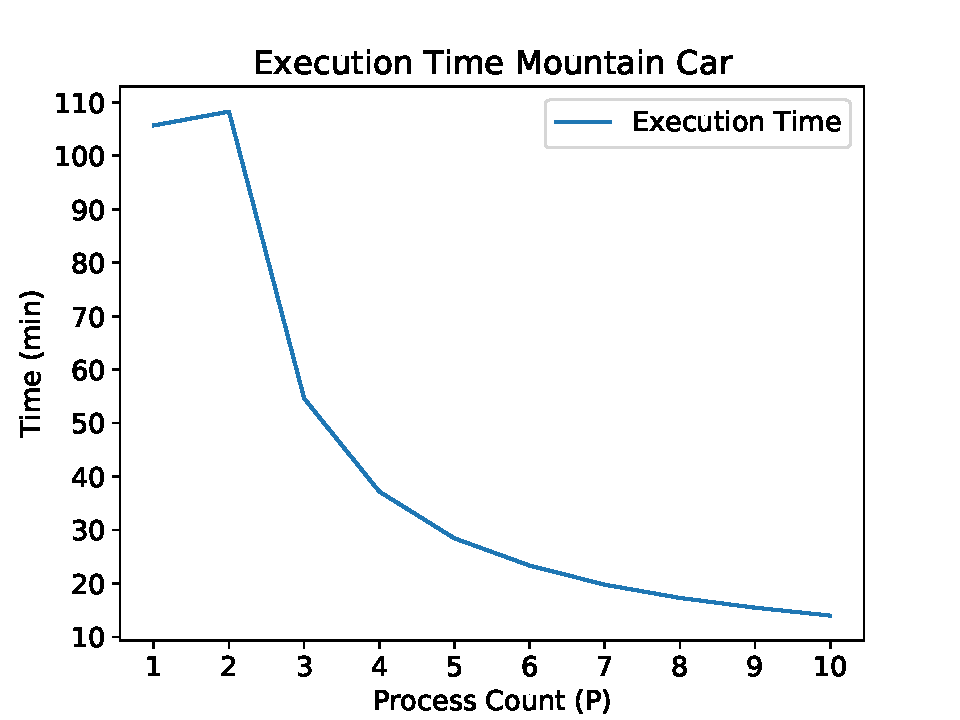
\includegraphics[width=0.7\textwidth]{./img/mountain_car_analysis/time_mountain_car_1_10.pdf} 
	\caption{Ausführungszeit des parallelisierten Verfahrens in der \emph{Mountain Car} Umgebung in Abhängigkeit zur Prozessanzahl}
	\label{fig:execution_time_mountain_car_1_10}
\end{figure}
\\\\
Für eine vollständige Bewertung des parallelisierten Verfahrens werden die in Kapitel \ref{subsec:basics_performance} vorgestellten Metriken \emph{SpeedUp} und Effizienz benötigt. Für eine bessere Einordnung der Ergebnisse werden diese nicht nur für die oben vorgestellte Konfiguration mit zehn Prozessen, sondern auch für Testdurchläufe mit zwei bis neun Prozessen berechnet. Diese werden im Folgenden mit derselben Konfiguration durchgeführt. Die hierbei entstehenden \ac{KNN} und Fitnesswerte sind identisch mit den vorherigen und sind daher nicht abgebildet. Die benötigte Ausführungszeit für das gesamte Verfahren in Abhängigkeit zur Anzahl an Prozessen ist in Abbildung \ref{fig:execution_time_mountain_car_1_10} dargestellt. Eine Besonderheit hierbei ist, dass die benötigte Ausführungszeit mit zwei Prozessen länger ist als die mit einem Prozess. Der Grund hierfür liegt in der gewählten \emph{Master-Slave} Architektur des parallelisierten Verfahrens. Mit einem Prozess wird das sequenzielle und andernfalls das parallelisierte Verfahren ausgeführt. Werden genau zwei Prozesse verwendet, gibt es einen \emph{Master} und einen \emph{Slave}. In diesem Fall ist die Ausführung langsamer als beim sequenziellen Verfahren, da der \emph{Master} im Rahmen der Parallelisierung nur die Kommunikation koordiniert, selbst aber keine Aufgabenpakete abarbeitet. Der \emph{Slave} führt alleine die Evaluation der Agenten durch. Dafür benötigt er dieselbe Zeit wie das sequenzielle Verfahren. Hinzu kommt der benötigte Kommunikationsaufwand für das Verteilen der Agenten und Sammeln von Fitnesswerten. Aufgrund der hierfür aufgewendeten Zeit ist das parallelisierte Verfahren mit zwei Prozessen langsamer als das sequenzielle Verfahren. Mit drei oder mehr beteiligten Prozessen sinkt die Ausführungszeit kontinuierlich. 
\begin{figure}[!h]
	\centering
	\begin{minipage}[]{0.49\textwidth}
		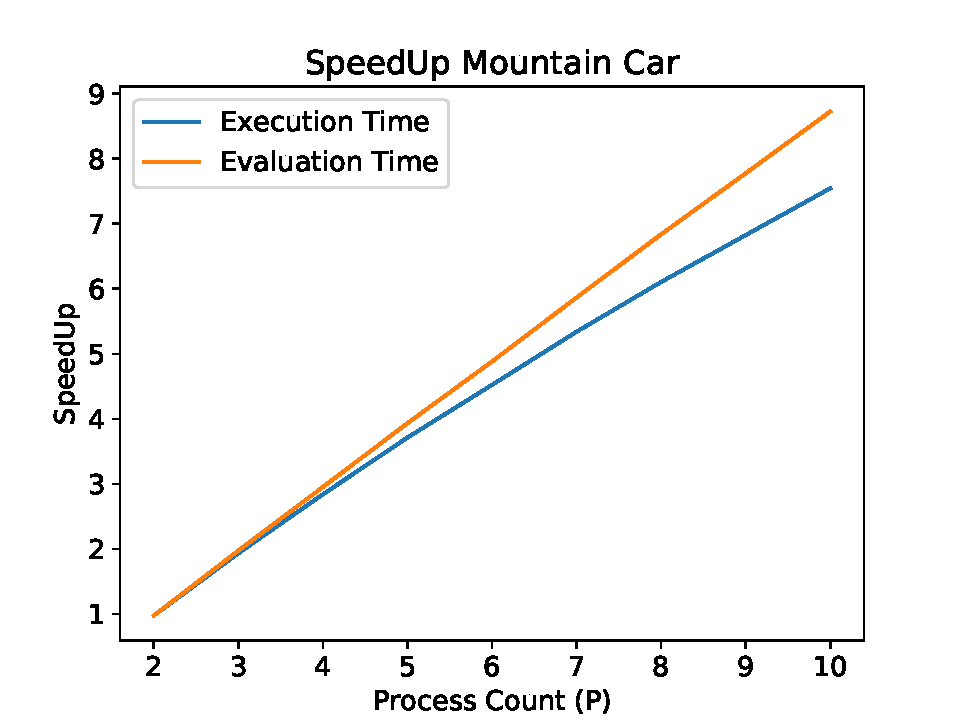
\includegraphics[width=1.0\textwidth]{./img/mountain_car_analysis/mountain_car_speedup_2_10.pdf} 
	\end{minipage}
	\hfill
	\begin{minipage}[]{0.49\textwidth}
		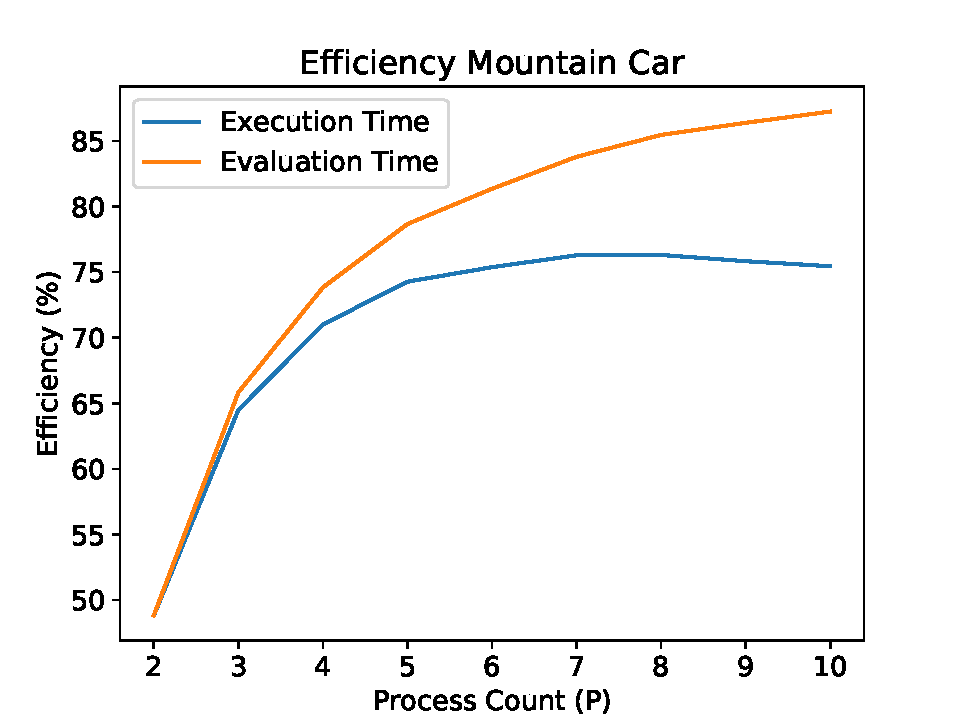
\includegraphics[width=1.0\textwidth]{./img/mountain_car_analysis/efficecny mountain_car_2_10.pdf} 
	\end{minipage}
	\caption{Links der \emph{SpeedUp}, rechts die dazugehörigen Effizienzwerte für die \emph{Mountain Car} Umgebung in Abhängigkeit zur Prozessanzahl}
	\label{fig:mountain_car_2_10_efficiency_speedup}
\end{figure}
\\\\
Anhand der Ausführungszeiten wird der \emph{SpeedUp} und die Effizienz des parallelisierten Verfahrens gemessen, welche eine Bewertung der Implementierung ermöglichen. Abbildung \ref{fig:mountain_car_2_10_efficiency_speedup} zeigt links die erreichten \emph{SpeedUps} und rechts die dazugehörigen Effizienzwerte in Abhängigkeit zur Anzahl an verwendeten Prozessen. In beiden Graphen sind jeweils die Metriken für die Evaluationsphase und das gesamte Verfahren dargestellt. Beim Testdurchlauf mit zehn Prozessen ist das parallelisierte Verfahren ungefähr um den Faktor $7.6$ schneller als das sequenzielle Verfahren. Dieses Ergebnis ist grundsätzlich höher als bei den vorherigen Testdurchläufen mit weniger Prozessen, entspricht aber nicht der Vorhersage von \emph{Amdahl's Law}. Laut diesem liegt der maximal erreichbare \emph{SpeedUp} mit zehn Prozessen in einem zu $98\%$ parallelisierbaren Programm bei ungefähr $8.5$. Durch die gewählte \emph{Master-Slave} Kommunikationsarchitektur ist zwischen dem erwarteten und tatsächlich erhaltenen Wert eine Differenz von $0.9$. Wie bereits beschrieben, unterstützt der \emph{Master} die \emph{Slaves} nicht bei der Evaluation, wird aber dennoch bei den Berechnungen berücksichtigt. Wird nur die Anzahl der \emph{Slave} Prozesse bei der Berechnung von \emph{Amdahl's Law} verwendet, ergibt sich ein maximaler \emph{SpeedUp} von $7.8$. Die restliche Differenz von $0.2$ entsteht durch den Kommunikationsaufwand. 
\begin{figure}[!h]
	\centering
	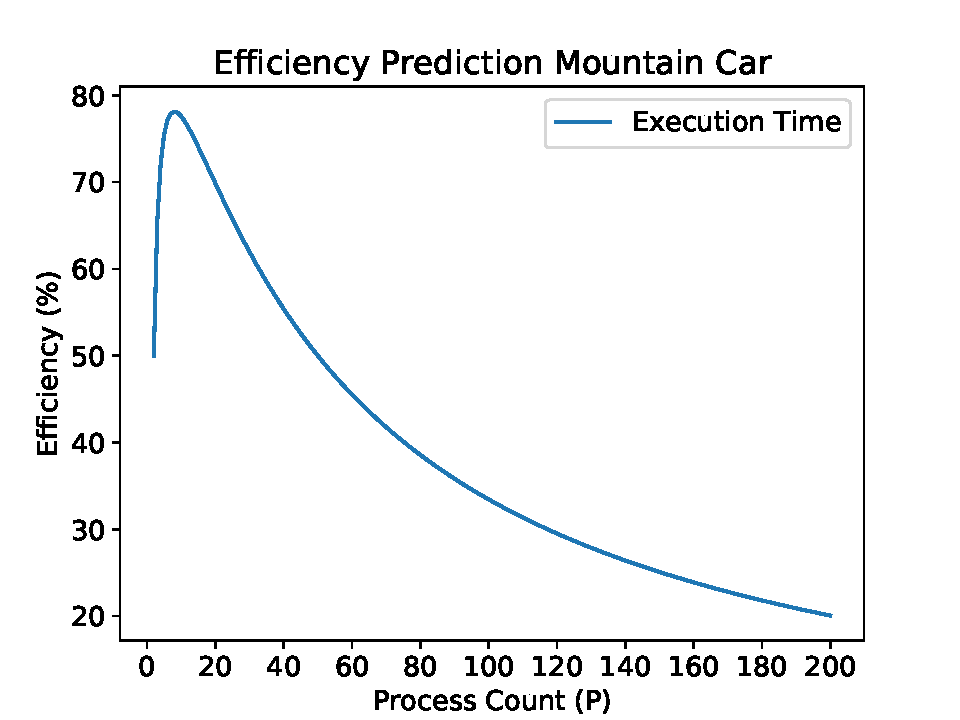
\includegraphics[width=0.7\textwidth]{./img/mountain_car_analysis/mountain_car_efficiency_prediction.pdf} 
	\caption{Erwartete Effizienz in der \emph{Mountain Car} Umgebung in Abhängigkeit zur Anzahl an Prozessen}
	\label{fig:mountain_car_efficiency_predidction}
\end{figure}
\\\\
Die in Abbildung \ref{fig:mountain_car_2_10_efficiency_speedup} rechts dargestellten Effizienzwerte beurteilen den \emph{SpeedUp} anhand der Prozessanzahl. Initial erzielt das parallelisierte Verfahren mit zwei Prozessen aufgrund der \emph{Master-Slave} Architektur eine geringe Effizienz. Mit je einem \emph{Master} und \emph{Slave} wird entsprechend der Abbildung \ref{fig:execution_time_mountain_car_1_10} eine etwas höhere Ausführungszeit im Vergleich zur sequenziellen Implementierung benötigt. Daher liegt der \emph{SpeedUp} bei ungefähr $0.98$. Entsprechend der Formel aus Kapitel \ref{subsec:basics_performance} ergibt die Berechnung der Effizienz einen Wert von $49\%$. Beim Hinzufügen weiterer Prozesse sinkt der Einfluss des \emph{Masters} auf das Ergebnis und die Effizienz steigt. Mit sechs bis zehn Prozessen wird ein Wert von über $75\%$ erreicht. Aufgrund des Graphen und \emph{Amdahl's Law} ist davon auszugehen, dass der Wert nicht weiter steigen, sondern durch Hinzufügen weiterer Prozesse letztendlich sinken wird. Abbildung \ref{fig:mountain_car_efficiency_predidction} zeigt die erwarteten Effizienzwerte für die \emph{Mountain Car} Umgebung mit einer \emph{Master-Slave} Architektur, wobei die Werte mit \emph{Amdahl's Law} berechnet worden sind. Auch in diesem Fall steigt die Effizienz anfangs stark an. Der höchste Wert von ungefähr $78\%$ wird mit acht Prozessen erreicht. Dies entspricht etwa dem tatsächlich erhaltenen Ergebnis. Hierbei wird die höchste Effizienz von $76\%$ ebenfalls mit acht Prozessen erreicht. Der Grund für das starke Absinken der Effizienz im weiteren Verlauf ist darin begründet, dass der \emph{SpeedUp} durch den sequenziellen Anteil von \emph{Amdahl's Law} immer gegen einen bestimmten Wert konvergiert. Die niedrigen Effizienzwerte entstehen, da der \emph{SpeedUp} nicht proportional zur Anzahl der Prozesse ansteigt.
\\\\
Es ist möglich, den \emph{SpeedUp} und die Effizienz nur für die parallelisierte \emph{Evaluation Time} zu berechnen, sodass der sequenzielle Teil des Verfahrens keinen Einfluss auf das Ergebnis hat. Die Ergebnisse hiervon sowie die des gesamten Verfahrens sind in Abbildung \ref{fig:mountain_car_2_10_efficiency_speedup} dargestellt. Der \emph{SpeedUp} der \emph{Evaluation Time} ist nahezu linear. Mit neun \emph{Slaves} bzw. zehn Prozessen wird ein \emph{SpeedUp} von $8.7$ erreicht. Diese guten Ergebnisse spiegeln sich in der Effizienz wieder. Diese ist anfänglich durch die \emph{Master-Slave} Architektur bei $49\%$, steigt aber stetig an. Mit zehn Prozessen liegt sie bei $87\%$. Prinzipiell kann der Wert weiter ansteigen, da der Einfluss des \emph{Masters} auf das Ergebnis mit zunehmender Prozessanzahl sinkt. Dennoch ist aufgrund der entstehenden Kommunikationszeit keine Effizienz von $100\%$ möglich. Bleibt bei der Effizienzberechnung der \emph{Master} Prozess unberücksichtigt, werden Ergebnisse zwischen $97\%$ und fast $99\%$ erreicht. Dies entspricht nahezu dem idealen Wert.

\subsection{Pendulum}
In diesem Kapitel wird die \emph{Pendulum} Umgebung mit dem parallelisierten Verfahren evaluiert und bewertet. Zusätzlich erfolgt ein Vergleich mit den Ergebnissen des vorherigen Kapitels. Hierzu wird das Optimierungsproblem zunächst in verschiedenen Testdurchläufen mit zwei bis zehn Prozessen optimiert und jeweils die \emph{Evaluation Time}, \emph{Reproduction Time} und \emph{Compose Offspring Time} erfasst. Die Konfiguration und der \emph{Seed} werden vom sequenziellen Verfahren übernommen, sodass alle Testdurchläufe dieselben Lösungen produzieren und ein Vergleich der Implementierungen möglich ist. Wie bei der \emph{Mountain Car} Umgebung, wird von jedem Raspberry Pi maximal ein Prozess ausgeführt. 
\begin{figure}[!htb]
	\centering
	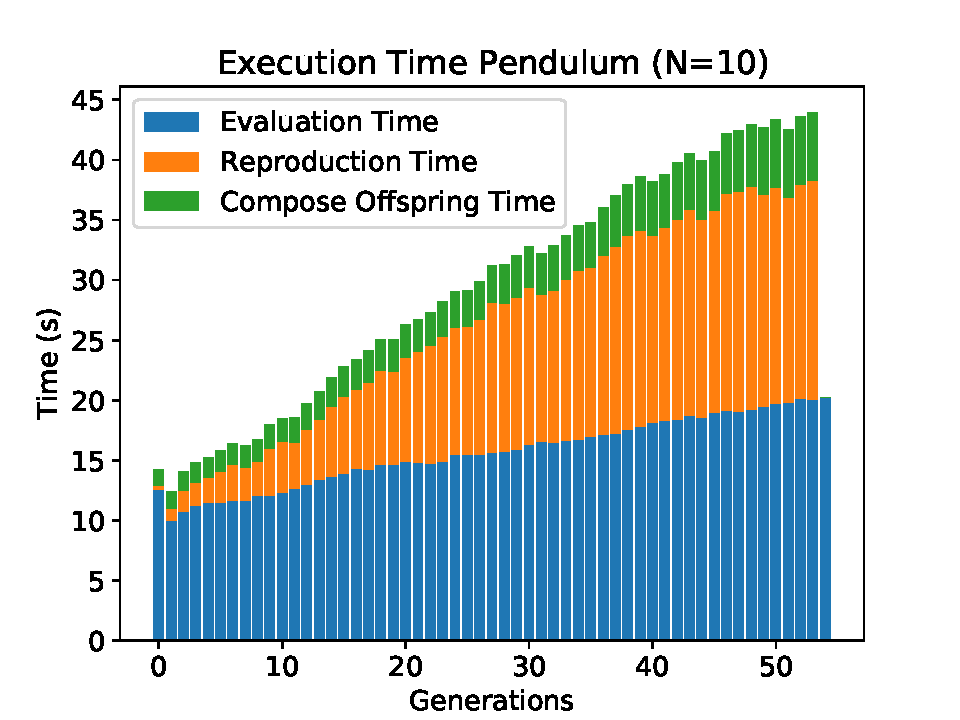
\includegraphics[width=0.7\textwidth]{./img/pendulum_analysis/pendulum_time_1_10core_10pi.pdf} 
	\caption{Ausführungszeit des \emph{Pendulum} Problems auf 10 \emph{Raspberry Pis} mit 10 Prozessen}
	\label{fig:pendulum_time_10cores_10pi}
\end{figure}
\\\\
Die Ergebnisse zeigen, dass die Fitnesswerte und die finalen \ac{KNN} identisch mit denen des sequenziellen Verfahrens sind, daher wird auf eine Abbildung verzichtet. Der Schwerpunkt der Analyse liegt auf den Ausführungszeiten. Diese sind von dem zuletzt durchgeführten Test mit zehn Prozessen in Abbildung \ref{fig:pendulum_execution_time_1_10} dargestellt. Wie bei der \emph{Mountain Car} Umgebung ist die \emph{Evaluation Time} der ersten Generation höher als die der zweiten. Der Grund hierfür liegt in der Initialisierung der einzelnen Prozesse. Die gesamte Ausführungszeit in diesem Test beträgt $27$ Minuten. Verglichen mit der Ausführungszeit der sequenziellen Implementierung von 138 Minuten ist dies eine Zeitersparnis von $111$ Minuten. Zuletzt ist bezüglich dieses Graphen hervorzuheben, dass die \emph{Evaluation Time} im Verlauf der Generationen nur leicht ansteigt und insgesamt $53\%$ der Ausführungszeit ausmacht. Der Anteil der beiden anderen Phasen ist anfänglich gering, steigt aber stark an und benötigt zusammen in den letzten Generationen mehr Zeit als die eigentliche Evaluation. Wie bereits beim sequenziellen Verfahren beschrieben, ist die hohe Anzahl an verschiedenen Spezies der Grund für die vergleichsweise hohe \emph{Reproduction Time}.
\begin{figure}[!htb]
	\centering
	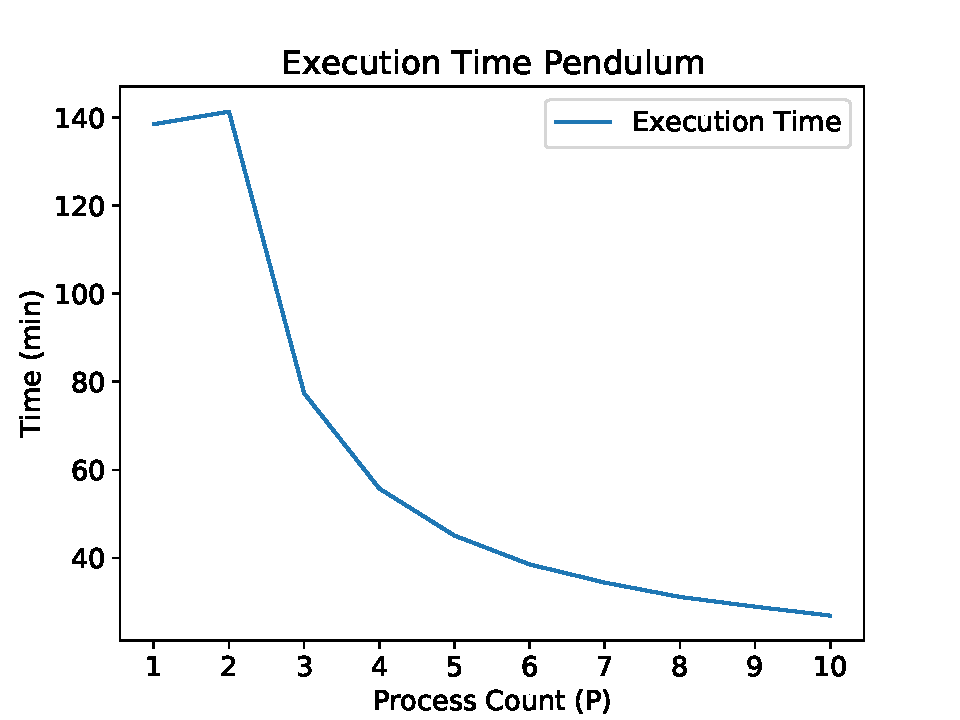
\includegraphics[width=0.7\textwidth]{./img/pendulum_analysis/pendulum_execution_1_1_10.pdf} 
	\caption{Ausführungszeit des parallelisierten Verfahrens in der \emph{Pendulum} Umgebung in Abhängigkeit zur Prozessanzahl}
	\label{fig:pendulum_execution_time_1_10}
\end{figure}
\\\\
Als nächstes wird der Verlauf der gesamten Ausführungszeit in Abhängigkeit zur Anzahl an Prozessen betrachtet. Diese sind in Abbildung \ref{fig:pendulum_execution_time_1_10} dargestellt. Prinzipiell ähnelt der Graph dem der \emph{Mountain Car} Evaluation. Mit zwei Prozessen steigt die Ausführungszeit im Vergleich zum sequenziellen Verfahren an. Wie in Kapitel \ref{subsec:mountain_car_optimzation} beschrieben, ist der Grund hierfür die gewählte \emph{Master-Slave} Architektur. Mit steigender Anzahl an Prozessen nimmt die Ausführungszeit kontinuierlich ab. Gegen Ende wird die Zeitersparnis mit zunehmender Anzahl an Prozessen immer geringer. Grund hierfür sind die sequenziellen Phasen des Verfahrens. 
\begin{figure}[!htb]
	\centering
	\begin{minipage}[]{0.49\textwidth}
		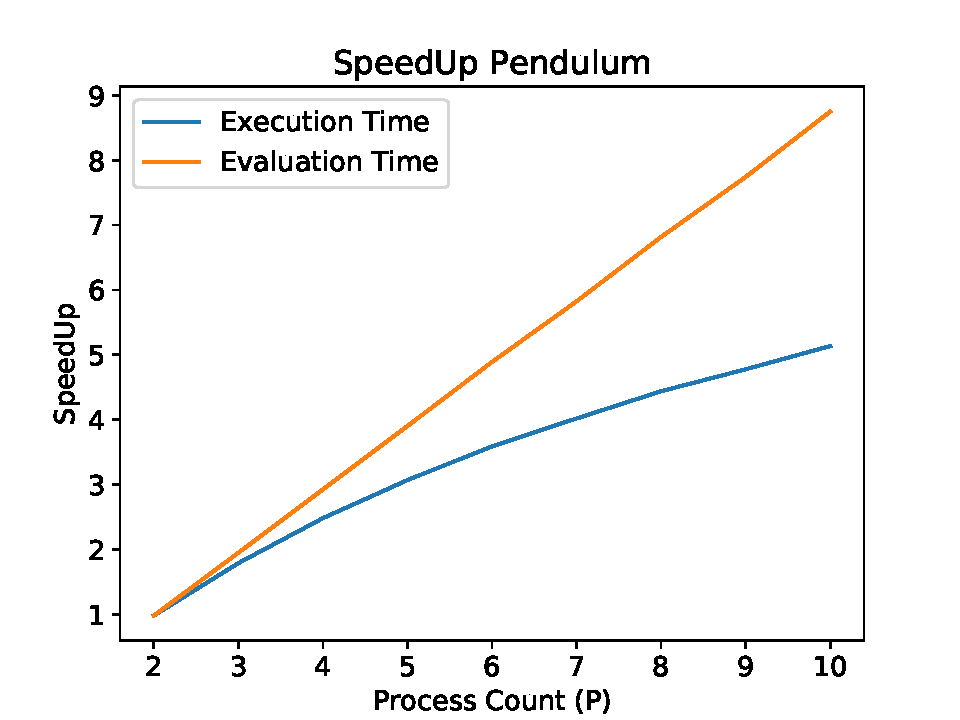
\includegraphics[width=1.0\textwidth]{./img/pendulum_analysis/pendulum_speedup1_2_10.pdf} 
	\end{minipage}
	\hfill
	\begin{minipage}[]{0.49\textwidth}
		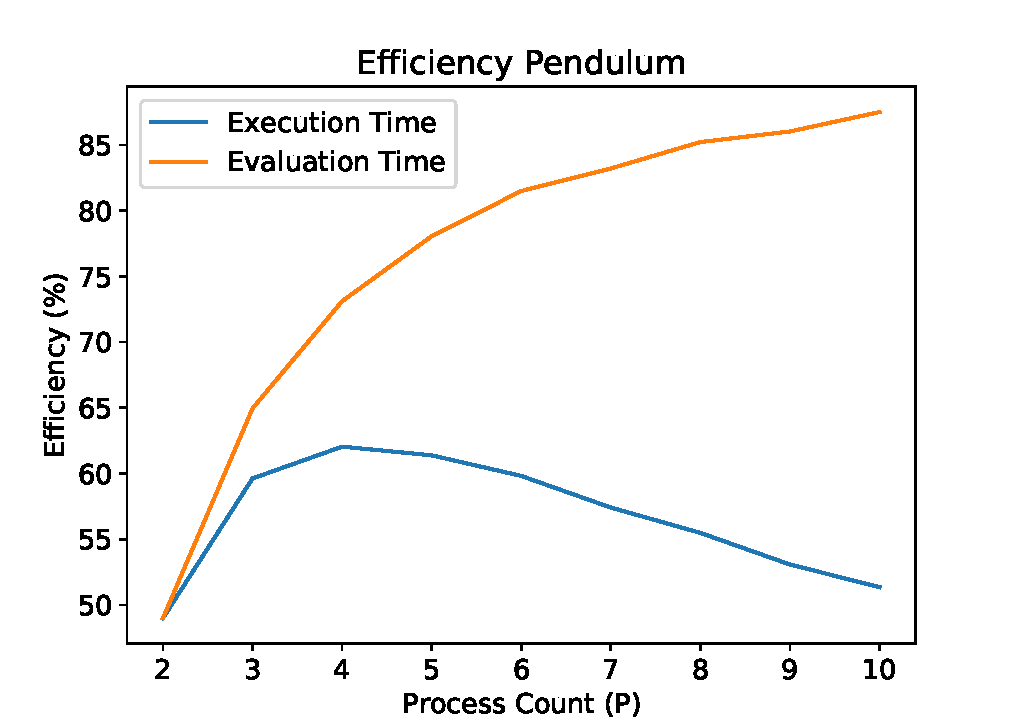
\includegraphics[width=1.0\textwidth]{./img/pendulum_analysis/efficiency_pendulum_2_10.pdf} 
	\end{minipage}
	\caption{Links der \emph{SpeedUp}, rechts die dazugehörigen Effizienzwerte für die \emph{Pendulum} Umgebung in Abhängigkeit zur Prozessanzahl}
	\label{fig:pendulum_2_10_efficiency_speedup}
\end{figure}
\\\\
Um die Ausführungszeiten und den Grad der Parallelisierung besser bewerten zu können, wird der \emph{SpeedUp} und die Effizienz für jeden Durchlauf berechnet. Die Ergebnisse sind in Abbildung \ref{fig:pendulum_2_10_efficiency_speedup} dargestellt, wobei jeweils die Werte für das gesamte Verfahren und die parallelisierte \emph{Evaluation Time} dargestellt sind. Auf Letzteres wird zuerst eingegangen. Der \emph{SpeedUp} für die Evaluationsphase ist nahezu konstant. Mit zehn Prozessen wird ein Faktor von $8.75$ erzielt. Dieses Ergebnis ähnelt dem der \emph{Mountain Car} Umgebung, bei der in dieser Phase ein Faktor von $8.7$ erreicht wird. Das Ergebnis ist insgesamt als sehr gut zu bewerten, da in der \emph{Master-Slave} Architektur mit zehn Prozessen bzw. neun \emph{Slaves} der maximal erreichbare \emph{SpeedUp} $9$ beträgt. Dies spiegelt sich auch in der Effizienz wieder. Bei der \emph{Master-Slave} Architektur liegt diese initial bei $49\%$, steigt aber stetig an. Mit zehn Prozessen wird ein Wert von $87\%$ für die Parallelisierung der \emph{Evaluation Time} erzielt. Die vergleichsweise schlechten initialen Messwerte sind durch die Berücksichtigung des \emph{Masters} bei der Berechnung zu erklären, da er selbst keine Agenten evaluiert. Derselbe Umstand tritt in der \emph{Mountain Car} Umgebung auf. Werden bei der Berechnung nur die zur Verfügung stehenden \emph{Slaves} betrachtet, liegt die Effizienz in allen Testdurchläufen bei ungefähr $97\%$, maximal bei $98\%$. Aufgrund der notwendigen Kommunikation wird keine Effizienz von $100\%$ erreicht. Zusammengefasst zeigen diese Ergebnisse, dass die Parallelisierung der \emph{Evaluation Time} in beiden Testdurchläufen sehr gute und konstante Ergebnisse liefert. Es ist davon auszugehen, dass trotz Hinzufügen von weiteren Prozessen die Effizienz bei einer entsprechenden Populationsgröße weiterhin hoch ist. Hierauf wird im Rahmen der Ergebnisse in Kapitel \ref{sec:results_optimziation} genauer eingegangen. In Abbildung \ref{fig:pendulum_2_10_efficiency_speedup} sind nicht nur der \emph{SpeedUp} und die Effizienz für die Evaluationsphase, sondern auch das gesamten Verfahrens dargestellt. Die hierbei erhaltenen Werte sind nicht so gut wie in der \emph{Mountain Car} Umgebung. Mit zehn Prozessen wird ein \emph{SpeedUp} von $5.1$ erreicht. Die \emph{Mountain Car} Umgebung erzielt im Vergleich hierzu noch einen Wert von $7.6$. Auch der Anstieg des \emph{SpeedUps} sinkt innerhalb der ersten zehn Generationen drastisch. Grund hierfür ist der Anteil der nicht parallelisierten \emph{Reproduction Time} und \emph{Compose Offspring Time}. Wie in Kapitel \ref{sec:parallel_strategies} veranschaulicht, ist in der \emph{Pendulum} Umgebung ein maximaler \emph{SpeedUp} von $11.\overline{1}$ möglich. Mit steigender Anzahl an Prozessen nähert sich das Ergebnis diesem Wert an.
\\\\
Entsprechend des \emph{SpeedUps} sind auch die Effizienzwerte weniger gut als in der \emph{Mountain Car} Umgebung. Anfangs liegt diese bei$42\%$, steigt danach an, erreicht mit vier Prozessen das Maximum von $62\%$ und sinkt danach kontinuierlich. Hierfür sind dieselben Gründe maßgeblich wie in der \emph{Mountain Car} Umgebung. Um die erhaltenen Ergebnisse besser einordnen zu können, werden mit \emph{Amdahl's Law} die zu erwartenden Effizienzwerte berechnet. Diese sind in Abbildung \ref{fig:pendulumr_efficiency_predidction} dargestellt. Aufgrund der unterschiedlichen Skalierung an den Achsen ist nicht offensichtlich, dass die gemessenen und idealen Ergebnisse sehr ähnlich sind. Die maximal erreichbare Effizienz von ungefähr $63.5\%$ tritt ebenfalls mit vier Prozessen auf. Die übrigen Effizienzwerte für zwei bis zehn Prozesse weichen weniger als zwei Prozentpunkte vom tatsächlich erhaltenen Ergebnis ab. 
\begin{figure}[!h]
	\centering
	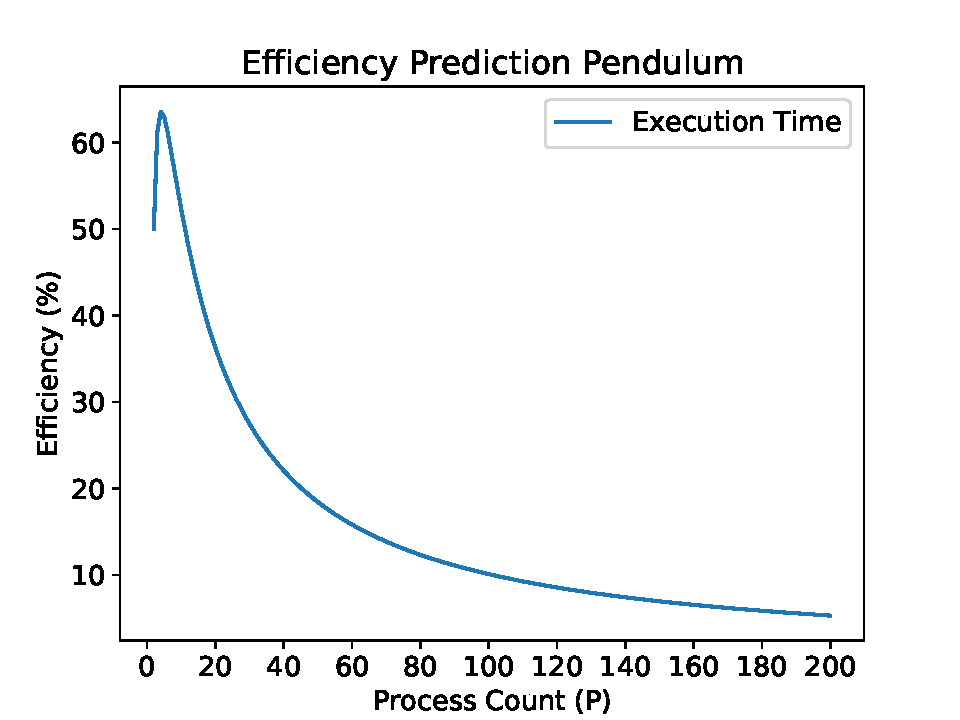
\includegraphics[width=0.7\textwidth]{./img/pendulum_analysis/pendulum_efficiency_prediction.pdf} 
	\caption{Erwartete Effizienz in der \emph{Pendulum} Umgebung in Abhängigkeit zur Anzahl an Prozessen}
	\label{fig:pendulumr_efficiency_predidction}
\end{figure}

\subsection{TITEL????}
Die bisherigen Testdurchläufe nutzen maximal zehn Prozesse gleichzeitig, einen auf jedem Raspberry Pi. Mit dieser Konfiguration werden insgesamt sehr gute \emph{SpeedUp} Ergebnisse erzielt. Prinzipiell ist es mit der bereits vorhanden Hardware möglich, die Ausführungszeit weiter zu reduzieren, da die \ac{CPU} der einzelnen Raspberry Pis nicht vollständig ausgelastet ist. Der Grund hierfür ist einerseits die Hardware und die Funktionsweise der Programmiersprache Python. In Kapitel \ref{sec:analysis_testsetup} ist beschrieben, dass der Raspberry Pi 4 über einen Quad-core ARM Prozessor verfügt. Das bedeutet, dass sich vier unabhängige Prozessoren auf derselben \ac{CPU} befinden, die parallel Programmcode ausführen können. Allerdings kann der Standard Python Interpreter dies nicht nutzen, da ein \ac{GIL} verwendet wird um die Sprache \emph{thread-safe} zu machen. Das bedeutet, dass nur ein \emph{Thread} gleichzeitig Programmcode ausführen kann. Existieren mehrere \emph{Threads} wechselt der Python Interpreter in regelmäßigen Abständen zwischen diesen, sodass jedem eine gewisse Ausführungszeit zusteht. Die Folge ist, dass alle \emph{Threads} eines Programms auf demselben Prozessor abgearbeitet werden und kein Reduzierung der Ausführungszeit möglich ist \cite{marowka2018python}. Für das Umgehen des \ac{GIL} gibt es verschiedene Ansätze, wobei eine Möglichkeit das Nutzen von \ac{MPI} ist. Die parallelisierte Implementierung kann in der vorgestellten Testumgebung auf zehn Raspberry Pis mit insgesamt $40$ Prozessen gestartet werden, sodass jeder Raspberry Pi vier Prozesse zugewiesen bekommt. Das Betriebssystem verteilt diese auf die vier verfügbaren Prozessoren und erzielt so eine parallele Ausführung. Bei dieser Umsetzung besitzen die einzelne Prozesse jeweils einen eigenen  immer noch einen eigenen \ac{GIL}, dieser interferiert jedoch mit dem von anderen Prozessen \cite{marowka2018python}.
\begin{figure}[!h]
	\centering
	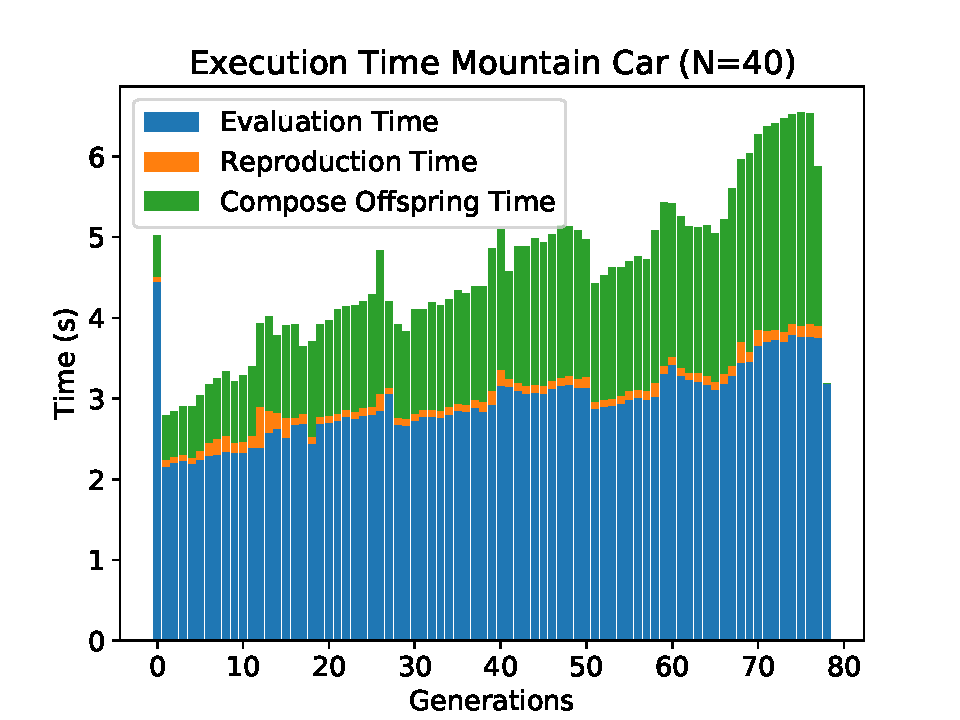
\includegraphics[width=0.7\textwidth]{./img/mountain_car_analysis/1413_time_40core_10pi.pdf} 
	\caption{Ausführungszeit des \emph{Pendulum} Problems auf 10 \emph{Raspberry Pis} mit 40 Prozessen}
	\label{fig:mountain_car_time_40core_10pi}
\end{figure}
\\\\
Um die Performance von diesem Szenario zu testen, werden die \emph{Mountain Car} und \emph{Pendulum} Umgebung erneut ausgeführt. Durch die vorherigen Ergebnisse ist zu erwarten, dass die Ausführungszeit der \emph{Evaluation Time} nahezu um den Faktor vier im Vergleich zu zehn Prozessen verringert wird. Abweichungen können durch andere Hintergrundprozesse oder das Betriebssystem entstehen, mit denen die verfügbaren Rechenkapazitäten geteilt werden müssen. Abbildung \ref{fig:mountain_car_time_40core_10pi} zeigt die gemessenen Ausführungszeiten für die \emph{Mountain Car} Umgebung mit $40$ Prozessen. Diese ist grundsätzlich im Vergleich zu den vorherigen Testdurchläufen gesunken. Insgesamt werden etwa sechs Minuten für die gesamte Ausführung benötigt, was einer Zeitersparnis von $99$ Minuten gegenüber dem sequenziellen Verfahren entspricht. Im Vergleich zu dem Testdurchlauf mit zehn Prozessen, ist die Ausführungszeit um 8 Minuten gesunken. Um eine Bewertung der Parallelisierung zu ermöglichen, wird der \emph{SpeedUp} und die Effizienz für das gesamte Verfahren sowie die \emph{Evaluation Time} berechnet.  Der \emph{SpeedUp} für das gesamte Verfahren beträgt im Vergleich zur sequenziellen Implementierung ungefähr $17.6$, die Effizienz liegt bei $44\%$. Diese Ergebnisse entsprechen nicht den Erwartungen. Nach \emph{Amdahl's Law} soll ein \emph{SpeedUp} von ungefähr $22.5$ erzielt werden, beziehungsweise von $22.1$ wenn der \emph{Master} Prozess bei der Berechnung ignoriert wird. Bei Betrachtung der \emph{Evaluation Time} sind die erhaltenen  Ergebnisse ebenfalls geringer als erwartet. Für diese Phase wird ein \emph{SpeedUp} von $26.7$ erzielt, was einer Effizienz von ungefähr $67\%$ entspricht. Selbst wenn der \emph{Master} Prozess ignoriert und nur die \emph{Slaves} betrachtet werden, liegt die Effizienz nur bei $68.4\%$. Dieses Ergebnis ist bedeutend geringer als die $97\%$ bis $99\%$, welche mit zwei bis zehn Prozessen erreichbar sind. Auch wenn bei der \emph{Pendulum} Umgebung etwas bessere Ergebnisse erzielt werden, skaliert die Leistung nicht wie erwartet. Der \emph{SpeedUp} für die \emph{Evaluation Time} beträgt ungefähr $29.6$ und ergibt eine Effizienz von $74\%$, beziehungsweise $76\%$ wenn der \emph{Master} nicht in die Berechnung miteinbezogen wird. Auch dies liegt über $20$ Prozentpunkte unter den vorherigen Ergebnissen. 
\\\\
Für den Leistungseinbruch können verschiedene Faktoren verantwortlich sein. Offensichtlich ist, dass an einer Stelle des Systems ein Ressourcenengpass entsteht. Um den Grund hierfür zu lokalisieren werden verschiedene Tests durchgeführt, auf deren Ergebnisse im Folgenden eingegangen. 

Zuerst wird der \emph{Master} Prozess untersucht. Dieser muss die Arbeitspakete mit einer geringen Latenz verteilen, sodass die \emph{Slaves} geringe Wartezeiten haben. Durch die hohe Anzahl an Prozessen, kann dies unter Umständen nicht gewährleistet werden. Um diese Behauptung zu überprüfen, wird das Optimierungsproblem angepasst. Jeder Agent muss bei der Evaluierung dieselbe Umgebung zehnmal absolvieren. Dies ändert nicht das Ergebnis, erhöhte aber die Ausführungszeit stark. Zwar ist die hierbei entstehende Last auf den \emph{Master} dieselbe, aber sie wird über eine größere Zeitspanne verteilt. Tritt bei diesem der Ressourcenengpass auf, sollte durch diese Maßnahme eine Steigerung der Effizienz erkennbar sein. Aber nach der Durchführung zeigen die Ergebnisse des Verfahrens nur eine geringfügige Steigerung. Daher kann der \emph{Master} Prozess als Engpass der Implementierung ausgeschlossen werden. 
\\\\
Stattdessen kommt die Hard- bzw. Software des Beowulf-Clusters in Frage. Um dies zu verifizieren, wird ein Testdurchlauf mit neun Prozessen und einer angepassten Konfiguration durchgeführt. Insgesamt werden drei Raspberry Pis verwendet, wobei auf einem der \emph{Master} Prozess und auf den anderen jeweils vier \emph{Slave} Prozesse gestartet werden. Mit dieser Konfiguration beträgt die Ausführungszeit des Verfahrens knapp $20$ Minuten und ein \emph{SpeedUp} von $5.3$ wird erzielt. Die \emph{Evaluation Time} macht hiervon $17.7$ Minuten aus. Diese Werte sind im Vergleich zu dem Durchlauf auf neun Raspberry Pis substanziell schlechter. Trotz derselben Anzahl an Prozessen ist die benötigte Ausführungszeit für das gesamte Verfahren $28\%$ höher und somit $4.4$ Minuten langsamer. Bei der Pendulum Umgebung treten ähnliche Ergebnisse auf. Daraus lässt sich folgern, dass sich mehrere Prozesse auf demselben Raspberry Pi teilweise gegenseitig blockieren und dadurch eine längere Ausführungszeit entsteht. 
\\\\
Zuletzt ist festzustellen, durch welche Komponenten des Algorithmus die Verzögerung entsteht. In einem ersten Schritt wird eine Umgebung des OpenAI Gyms untersucht. Abbildung \ref{fig:test_bottleneck} zeigt den erstellten Test. Es wird zuerst die \emph{Pendulum} Umgebung initialisiert und danach werden $160.000$ Zufallsaktionen ausgeführt. Die hierfür benötigte Zeit wird gemessen und am Ende ausgegeben. Der Test wird zunächst mit einem Prozess ausgeführt und hat eine gemessene Laufzeit von $75.6$ Sekunden. Danach wird der Test mit vier Prozessen auf einem Raspberry Pi wiederholt. Der zu leistende Rechenaufwand wird in diesem Fall nicht geteilt und daher sollte jeder Prozess $160.000$ Zufallsaktionen in einer lokalen Umgebung ausführen und dafür dieselbe Zeit benötigten. Allerdings zeigen die Messergebnisse einen Anstieg von $27\%$ auf $95.5$ Sekunden. Ein ähnlicher Test wird mit einem \ac{KNN} durchgeführt. Mit einem Prozess werden hierfür $73$ Sekunden benötigt. Beim der Ausführung mit vier Prozessen steigt die Laufzeit um ungefähr $9.5\%$ auf 80 Sekunden an. Da in den letzten beiden Tests keine Nachrichten ausgetauscht werden, ist zu schließen, dass die zuvor festgestellten Leistungseinbrüche mit $40$ Prozessen nicht nur einen zu großen Kommunikationsaufwand sondern vor allem durch die verwendeten Optimierungsprobleme entstehen. 
\begin{figure}
	\begin{python}
		import gym
		import time
		
		env = gym.make("Pendulum-v0")
		env.reset()
		
		start_time = time.time()
		for _ in range(160000):
			env.step(env.action_space.sample())
		
		time_required = time.time() - start_time
		print(time_required)
	\end{python}
	\label{fig:test_bottleneck}
	\caption{Python Programmcode zum Überprüfen der Parallelisierung des OpenAI Gyms}
\end{figure} 


% Prozentsatz an Abweidung nicht parllelisierter Verfahren, 
% Zuerst Ergebnisse 10 Pis, mit Verifizierung Funktionalität und allgemeines Ergebnis
% Eingehen dass Master Pi keine Abarbeitugn übernimmt sondern nur Koordination
% Zeiten von anderen Phasen weichen ab, daher kann es zu varianzen kommen
% Allgemeine Laufzeit des Verfahrens und Laufzeit des evaluierten Verfahren anzeigen
% Vergleich mit Amdahls Law? +++++ 


% Auch Lunar Lander
\section{Ergebnisse}
\label{sec:results_optimziation}
% !TeX spellcheck = de_DE
\chapter{Zusammenfassung und Ausblick}
In dieser Arbeit ist das Verfahren \ac{NEAT} analysiert und für ein verteiltes System parallelisiert worden. Die Ergebnisse der vorherigen Kapitel werden im Folgenden zusammengefasst. Zusätzlich sind einige Vorschläge für zukünftige Weiterentwicklungen gegeben, die nicht im Rahmen dieser Arbeit umgesetzt sind.  

\section{Ergebnis}
Die erste Anforderung an diese Arbeit ist die Implementierung des sequenziellen Verfahrens. Hierfür ist die Sprache Python gewählt worden, da sie im Bereich maschinelles Lernen weit verbreitet ist und viele Bibliotheken bietet. Eine hiervon ist das OpenAI Gym, welches bei der Analyse und Evaluation genutzt wird. Die generelle Softwarearchitektur ist in Kapitel \ref{chap:software_architecture} beschrieben. Sie ist darauf ausgelegt, eine einfach zu nutzende Schnittstelle zu bieten. Dadurch können verschiedene Optimierungsprobleme schnell und effizient implementiert werden. Ein weiterer wichtiger Aspekt ist, dass das Ergebnis des Verfahrens durch einen \emph{Seed} beeinflusst wird. Dadurch ist das Wiederholen und Vergleichen von Testergebnisse mit der später erstellten parallelisierten Implementierung möglich. Zuletzt ist bei der Softwarearchitektur zu verdeutlichen, dass das optimierte \ac{KNN} und die Testergebnisse gespeichert und visualisiert werden können. Dies ist unter anderem notwendig, wenn das \ac{KNN} in einer produktiven Umgebung eingesetzt werden soll.
\\\\
Kapitel \ref{chap:analysis} beschreibt die Analyse des sequenziellen Verfahrens. Dies entspricht der zweiten Anforderung an diese Arbeit. Zuerst wird die korrekte Funktionalität des implementierten Algorithmus mit dem XOR-Problem überprüft. Mit der Konfiguration aus der originalen Publikation werden ähnliche Ergebnisse erzielt, wie sie von den Autoren beschrieben sind. Inspiriert durch das Paket \emph{neat-python} werden die Konfiguration und das Verfahren modifiziert. Dadurch sinkt die Anzahl der benötigten Generationen zum Lösen des XOR-Problems beträchtlich. Im nächsten Schritt der Analyse wird die Ausführungszeit des sequenziellen Verfahrens in verschiedenen Beispielen erfasst. Das XOR-Problem wird wegen einer zu geringen Komplexität hierfür nicht verwendet. Es werden die \emph{CartPole}, \emph{MountainCar} und \emph{Pendulum} Umgebung des OpenAI Gym ausgewählt. Bei allen drei Umgebungen kann die Fitnessfunktion mit den zur Verfügung gestellten \emph{rewards} implementiert werden. Die Testdurchläufe zeigen, dass die initiale Generation die \emph{CartPole} Umgebung bereits lösen kann und sie daher für die weiteren Tests ungeeignet ist. Bei den anderen beiden Umgebungen werden die Ausführungszeiten gemessen. Hierbei wird zwischen der \emph{Evaluation Time}, \emph{Reproduction Time} oder \emph{Compose Offspring Time} unterschieden. Die \emph{Evaluation Time} misst die benötigte Zeit zum Evaluieren aller Agenten. Diese macht in beiden Testumgebungen mit Abstand den größten Anteil an der gesamten Laufzeit des Algorithmus aus.
\\\\
Die letzte Anforderung an diese Arbeit ist die Optimierung, welche in Kapitel \ref{chap:optimization} beschrieben ist. Hierbei wird der Fokus auf die Parallelisierung der \emph{Evaluation Time} gelegt, da hierbei die größte Zeiteinsparung möglich ist. Es wird eine \emph{Master-Slave} Architektur mit \ac{MPI} implementiert. Der \emph{Master} verteilt Arbeitspakete, die je einen Agenten enthalten und von den \emph{Slaves} evaluiert werden. Der Vorteil von diesem Ansatz ist, dass sowohl das \ac{KNN} als auch das Optimierungsproblem parallelisiert ausgeführt werden. Der dabei entstehende Kommunikationsaufwand ist sehr gering und ermöglicht insgesamt eine gute Parallelisierung. Zusätzlich kann die bereits vorhandene Struktur einfach erweitert werden, sodass auch die Parallelisierung der \emph{Reproduction Time} oder \emph{Compose Offspring Time} möglich ist. Das Verfahren wird auf einem verteilten System ausgeführt. Hierfür wird ein Beowulf-Cluster aus zehn Raspberry Pis erstellt. Neben geringen Kosten und einer platzsparenden Unterbringung bietet dies den Vorteil, dass alle Geräte identisch konfiguriert sind. Das vereinfacht den Vergleich zwischen der sequenziellen und parallelisierten Implementierung. Um die Effizienz der Parallelisierung zu messen, werden die zuvor durchgeführten Tests wiederholt und die Ausführungszeit erfasst. Auf jedem beteiligten Raspberry Pi wird hierzu ein Proezss ausgeführt. Bei Verwendung von zwei oder mehr \emph{Slaves} wird die Ausführungszeit stark reduziert. Für eine Bewertung der Parallelisierung sind der \emph{SpeedUp} und Effizienzwert berechnet worden. Die erhaltenen Ergebnisse entsprechen nahezu den idealen Werten, die mit \emph{Amdahl's Law} berechnet sind. Werden nur die \emph{Slaves} betrachtet, ist die \emph{Evaluation Time} mit einer Effizienz von $97\%$ parallelisiert. Dies ist ein sehr gutes Ergebnis und wird unter anderem durch die effiziente Kommunikation ermöglicht. Für ein Population mit $n$ Mitgliedern müssen nur $2 \cdot n$ Nachrichten versendet werden. Zusätzlich ist in Kapitel \ref{chap:optimization} demonstriert, dass mit \ac{MPI} das \ac{GIL} von Python umgegangen werden kann. Es können alle $40$ Prozessoren des erstellten Beowulf-Clusters vollständig ausgelastet werden. Allerdings sind die dabei entstehenden \emph{SpeedUp} Werte niedriger als durch die vorherigen Tests angenommen. Der Grund ist, dass sich mehrere Prozesse auf einem Gerät sich gegenseitig blockieren bzw. behindern. Die genaue Ursache hiervon kann im Rahmen dieser Arbeit nicht untersucht werden. Die Tests zeigen jedoch, dass dies nicht primär durch das implementierte Verfahren entsteht sondern unter anderem durch das OpenAI Gym.
\\\\
Insgesamt haben die erzielten \emph{SpeedUp} und Effizienzwerte die Erwartungen übertroffen. Durch eine gute Parallelisierung können neuroevolutionäre Algorithmen einen entscheidenden Vorteil gegenüber dem Backpropagation Algorithmus und seinen Derivaten bieten. Der große Vorteil ist, dass sowohl das \ac{KNN} als auch das Optimierungsproblem parallelisierbar sind. Durch die erfassten Ergebnisse ist zu schließen, dass mit steigender Anzahl an Prozessoren die Ausführungszeit weiter sinken wird. Die zuletzt vorgestellte \emph{Lunar Lander} Umgebung verdeutlicht nochmals, wie groß die tatsächliche Einsparung ist. Verfahren die auf einem Raspberry Pi 4 mehrere Tage dauern, können auf zehn Geräten in wenigen Stunden beendet werden. Für eine vollständige Bewertung ist auch zwei Nachteile zu nennen. Gibt es mehr Prozesse als Agenten in einer Generation, kann nicht jedem ein Arbeitspaket zugewiesen werden. In diesem Fall kann durch Hinzufügen von weiteren Rechenressourcen keine Reduzierung der Ausführungszeit erreicht werden. Jedoch ist es in einer solchen Situation möglich die Populationsgröße entsprechend anzupassen. Mit einer größeren Population können mehr Lösungsansätze gleichzeitig evaluiert werden was indirekt schneller zu einer Lösung führen kann. Der zweite Nachteil betrifft \ac{NEAT} direkt. Grundsätzlich werden mit diesem Algorithmus beeindruckende Ergebnisse erzielt. Jedoch können die vorgestellten Arten der strukturellen Mutation nicht ausreichend sein um große \ac{KNN} in einer kurzen Zeit zu entwickeln. In diesem Fall kann das HyperNEAT Verfahren aus Quelle \cite{stanley2009hyperneat} verwendet werden. Dieses basiert auf \ac{NEAT} und ermöglicht die Entwicklung von größeren \ac{KNN}. Die in dieser Arbeit vorstellten Parallelisierungsstrategie bezieht sich vor allem auf die Evaluationsphase und kann daher auf verschiedene neuroevolutionäre Algorithmen angewendet werden.

\section{Weiterentwicklung}
Das implementierte Projekt bietet die Grundlage für verschiedene Erweiterungen. In Kapitel \ref{sec:parallel_strategies} ist bereits die Integration von Bibliotheken wie Tensorflow und PyTorch vorgestellt. Mit diesen kann die Aktivierungszeit von \ac{KNN} stark reduziert werden und auch die Nutzung von \acp{GPU} wird ermöglicht. Für einen noch besseren \emph{SpeedUp} müssen die Funktionen der  \emph{Reproduction Time} und \emph{Compose Offspring Time} ebenfalls parallelisiert werden. Denn durch \emph{Amdahl's Law} ist erkennbar, dass die Phasen zwar beim sequenziellen Verfahren nur einen geringen Prozentsatz der Ausführungszeit benötigen, aber bei steigender Parallelisierung zunehmend zum limitierenden Faktor werden. Prinzipiell ist es mit der \emph{Master-Slave} Architektur möglich beliebig viele weitere Funktionen mit geringem Aufwand zu parallelisieren. 
Die Funktionen für die Mutation der Gewichte und die Rekombination zum Erzeugen von Nachkommen bieten sich für eine Parallelisierung an. Für letzteres kann der \emph{Master} Arbeitspakete mit je zwei Agenten erstellen. Die \emph{Slaves} führen für diese die Rekombination aus und geben den neu erstellten Agenten als Ergebnis zurück. Selbes Prinzip kann auf die Mutation der Gewichte angewendet werden. Andere Funktionen hingegen können nur schlecht oder teilweise parallelisiert werden. Ein Grund hierfür können globale Variablen sein, wie es im Fall der strukturellen Mutationen mit den Innovationsnummern ist. Die Funktion zum sortieren der Agenten in die Spezies kann teilweise parallelisiert werden. Die Zuweisung der Agenten in die bestehenden Spezies kann parallel geschehen, das Erzeugen von neuen Spezies hingegen muss sequenziell durchgeführt werden. Insgesamt ist der Aufwand für die Parallelisierung dieser Phasen bedeutend höher und wird wahrscheinlich dieselben \emph{SpeedUp} Ergebnisse liefern wie die \emph{Evaluation Time}. Daher ist die Parallelisierung dieser Phasen häufig erst sinnvoll, wenn durch hinzufügen von weiteren Prozessen die Ausführungszeit der \emph{Evaluation Time} nicht weiter reduziert werden kann. 


%Da die Ausführungszeit des Algorithmus für das XOR-Problem nicht repräsentativ ist, werden drei andere Optimierungsprobleme aus dem OpenAI Gym für die Analyse verwendet. Dabei ist darauf zu achten, dass die Umgebungen nicht zu komplex sind, da die Implementierung auf einem Raspberry Pi 4 ausgeführt wird, der selbst nur eine vergleichsweise geringe Rechenleistung bietet. Aus diesen Gründen werden die Standardumgebungen \emph{CartPole}, \emph{MountainCar} und \emph{Pendulum} ausgewählt. Bei den Tests zeigt sich, dass nur die zwei letzteren geeignet sind. 
%\\\\
%Die \emph{CartPole} Umgebung kann mit zufällig erstellten \ac{KNN} sind bereits in der initialen Generation \ac{KNN} vorhanden, die das Optimierungsproblem lösen. Für die \emph{MountainCar} und \emph{Pendulum} Umgebung werden dem \ac{KNN} einige strukturelle Innovationen hinzugefügt, bis das Optimierungsproblem gelöst wird.  



% Struktur
% Stellvertretend NEAT für Neuroevolutionäre Algorithmen analysisiert
% Implementierung des sequenziellen Verfahrens als Bibliothek. Viele Funktionen extern, sodass in beiden beiden Implementierungen wiederverwendet werden können Ist in Kapitel So und So beschrieben. Wichtige Eigenschafte, Seed basiert, Einfach für verschiedene Probleme anzupassen, Unterteilung der Laufzeit in 3 Bereiche. Speichern und Laden von Ergebnissen möglich, Sprache Python ausgewählt für schnelle Entwicklung, viele Pakete möglich

% Analyse
% Laufzeit von sequenziellem Verfahren erfassen. Zuvor korrekte Implementierung von NEAT überprüfen mit XOR, Dabei anfänglich etwas schlechtere Ergebnisse als orginale Publukation, danach aber bedeutend besser. 
% 3 Testumgebungen inital durchgeführt aus dem OpenAI Gymfür gute Vergleichbarkeit. Pole Balancing, zu einfach, zufälliges KNN kann das Problem lösen, Mountain Car schwieriger, KNN mit Hidden Neuronen wird entwickelt, Laufzeit zeigt, dass Evaluation der größte Faktor ist. Umfasst KNN und Umgebung, Phasen des NEAT algorithmus eher weniger großen Einfluss. Gleiches zeigt sich in Pendulum. 

% Optimierung
% Es soll hauptsächlich die Evaluation Time parallelisiert werden, da das mit abstand der gröte Faktor ist. Prinzipiell verschiedene Optimierugnsstrategien, in dieser Arbeit soll Cide parallelisiert werden. Ziel ist die Ausführung auf einem Cluster zu ermöglichen, wie beispielsweise im HPC Computing. Architektur wird Master Slave gewählt, für einface Kommunikaktion und Erweiterbarkeit. Für die Testumgebung ist ein Raspberry Pi beowulf cluster erstellt worden, Vorteil: Alle exakt dieselbe Hardware, theoretisch mit 10 Geräten 10 Fache Rechenleistung. Vergleich einfach möglich. 
% Durchführen der Mountain Car und Pendulum Umgebung. Wichtige Erkenntnis, beide Verfahren erzegen exakt dieselebn lösungen, somit auch dieselebn Rechenschritte. Vergleich sinvoll. Tests mit einem Prozess pro Pi durchgeführt, Sehr gut eErgebnisse. SpeedUp und Effizienz entsprechen erwarteten Werten. Auswertung Evaluation Time ergibt, und nur Slaves, $97%$ eEffitienz. Ergebnis nahezu ideal.
%Allerdings, zeigen sich auch Grenzen der Parallelisierung.
% Irgendwann ist Reduzierung der Ausführungszeit nicht mehr Lohnenswert. Da Zeiteinsparung immer geringer wird, aber benötigte prozessoren stark ansteigen.  Grund: Sequenzieller Anteil. Müsste auch parallelisiert werden.  Ansätze hierzu in Kaputel SO und SO

% MPI erlaut umgehen von GIL, Mit der Implementierung auch möglich. Alle 40 Prozesse genutzt. Problem, Prozesse auf demselben Gerät behindern sich gegenseitig. Ergebnis in dem TestSetup: Verfahrne insgesamt schneller, also definitiv Vorteil: Rechenkapazität ist vorhandne, kann aber sonst nicht genutzt werden. Aber nicht so gut wie erwartet. Daher weitere Untersuchungen notwendig

% Lunar Lander als letztes zeigt ENtwicklung von generellen Lösung. In vielen Fällen wir dEvaluation dadurch noch aufwändiger, aber Code profiziert noch mehr von PArallelisierung. Daher Wahl der Evaluation Time prinzipiell gut und wicthig

% Grenze der Parallelisierung: Prozesse = Größe der Generation: Jeder Prozess arbeitet einen Agenten ab. Danach keine Aufteilung möglich. Eine Option in diesem Fall: Populationsgröße vergrößeren. Ähnlich zu Gustafsons Law, wird dadurch dem System höhere Arbeitslast gegeben. Dadurch kann schneller Lösung gefunden werden, da größerer Suchraum abgetastet wird, Aber!! Kann auch nichts bringen, wenn Bsp: neue Struturen benötigt werden. Die müssen erst entwickelt werden.

% Übertragen der Ergebnisse auf andere Algorithmen absolut möglich, jeder NE wird eine Evaluationsphase haben. Häufig wird diese ebenfalls der aufwändigste Faktor sein. Ergebnisse decken sich mit Quelle so und so. Eventuell mögliche Erweiterung für HyperNEat: Dies kann größere KNN entwickeln als andere Verfahren. Eventuell Größe irgendwann ein PRoblem? Bei Übertragung mit MPU

% Weiterentwicklung:
%Trotz guter Ergebnisse, einige Grenzen. Das erste Ergebnis ist die Reproduction and Compose OffSpring Time. Sind limiterender Faktor bei der Prallelisierung. Werden diese auch Parallelisiert, können laut Amhdals law bedeutend bessere Ergebnisse erzieltz werden. Nachteil ist, diese Phasen brauchen globale Variablen, bzw. Aktionen die nacheinander ausgefüht werden müssen, Parallelisierung schwieriger, aufwändiger?  nicht effizienz. Einige Ideen: Mutation: prinzipiell einfach, aber bei den Anforderungen in dieser Arbeit zusätzliche Schwierigkeit wegen Seed basiertem Verfahren. Jeder Prozess muss denselben Seed verweden, da sich sonst Ergebnisse unterscheiden. Ist keine Vergleich möglich, gut umsetzbar und mit Master Slave Architektur leicht integrierbar
% Reproduction Schwieriger: Innovationsnnummern benötigen gloabelen Counter. Bei jeder strukturellen Mutation muss dieser synchronisiert werden, sehr zeitaufwändig. Ein Ansatz: Innovationsnsummern werden nicht als Zahl benötigt, sondern als eindeutige ID: Eventuell nutzen von HashFunktion? Eingabe so und so, Bestimmt Innoationsnummer von Verbindungen / Neuron. VOrteil: keine Synchronsiation udn dieselben Mutationen bekommen denselben Wert zugewiesen.+
% Umseten der Rekombination ist wie Mutation theoretisch möglich, Zwei Elternteile an Slaves verteilen, bringen neuen Agent zurück, idealerweise mutiert.
% Problem: Soriteren der Agenten in Spezies. Aufwändiger Teil gewesen: Problem: Neue Spezies erstellen, muss global synchronsiert sein. Nur teilwesie Parallelisierung möglich. Agenten werdne wenn möglichj in Spezies soritert. Agenten für die keine Spezies gefunden wird, ignorieren und erst am Ende Sequenziell zuweisen. Dadurch teil Parallelisierung.

% Problem bei all diesen Parallelisierungen ist, sehr speziell für NEAT. Parallelisierung der Evaluatino kann hingegen leicht auf andere angewendet werden. Tatsächlich Zeitersparnis fragwürdig? Zumindest inital liegt fokus mehr auf der Evaluation TIme.

% Weitere Erweiterung Tensorflow oder PyTorch: Könnne mit INterface NN implementiert werden, schnellere AKtivierung von KNN. In diesem Fall auch Integratoin von GPUs sinvoll, da auf diesen KNN Aktivierung noch schneller berechnet werden kann. A




% TODO PRint biliography
% Bibliography
%\printbibliography[
%heading=bibintoc, 
%title={Quellenverzeichnis}
%]

% statutory declaration
% !TeX spellcheck = de_DE
\chapter*{Eidesstattliche Erklärung}
\addcontentsline{toc}{chapter}{Eidesstattliche Erklärung}

Ich versichere, dass ich die vorliegende Thesis ohne fremde Hilfe selbstständig verfasst und nur die angegebenen Quellen benutzt habe.\\
\\\\\\\\

\noindent\begin{tabular}{ll}
	\makebox[2.5in]{\hrulefill} & \makebox[2.5in]{\hrulefill}\\
	Ort und Datum & Unterschrift\\[8ex]% adds space between the two sets of signatures
\end{tabular}

\end{document}